\documentclass[a4paper, 11pt]{article}

\usepackage[version=3]{mhchem}
\usepackage{siunitx}
\usepackage{graphicx}
\usepackage{amsmath}
\usepackage[total={16cm,25cm}, top=3cm, left=2.5cm, includefoot]{geometry}
\usepackage{pgfplots}
\usepackage{float}
\usepackage{amsfonts}
\usepackage{booktabs}
\usepackage{easytable}
\usepackage{mathtools}
\usepackage{comment}
\usepackage[makeroom]{cancel}
\renewcommand{\figurename}{Obrázek}
\renewcommand{\refname}{Zdroje}
\renewcommand{\tablename}{Tabulka}
\renewcommand{\contentsname}{Obsah}

\setlength\parindent{0pt}
\setcounter{section}{0}
\renewcommand{\labelenumi}{\alph{enumi}.}
\usepackage{xcolor}
\definecolor{light-gray}{gray}{0.95}
\newcommand{\code}[1]{\colorbox{light-gray}{\texttt{#1}}}
\newcommand{\logoCVUT}{
\includegraphics[width = 0.5\textwidth]{img/symbol_cvut_konturova_verze_cb.pdf}}
\newcommand{\logoFJFI}{
\includegraphics[width = 0.4\textwidth]{img/fjfi_logo.png}}

\begin{document}
% \section*{Seznam použitých veličin}
\addcontentsline{toc}{section}{Seznam použitých veličin}
\markboth{Seznam použitých veličin}{Seznam použitých veličin}

\renewcommand{\arraystretch}{1.2}
\begin{table}[H]
\begin{tabular}{p{1cm}l}
  $\Phi$          & hustota toku neutronů (1/cm$^2$s) \\
\end{tabular}
\end{table}
\renewcommand{\arraystretch}{1}

% \section*{Seznam použitých zkratek}
\addcontentsline{toc}{section}{Seznam použitých zkratek}
\markboth{Seznam použitých zkratek}{Seznam použitých zkratek}

\renewcommand{\arraystretch}{1.2}
\begin{table}[H]
\begin{tabular}{p{1cm}l}
  AZ           & aktivní zóna \\
\end{tabular}
\end{table}
\renewcommand{\arraystretch}{1}


% titulní strana
\thispagestyle{empty}

\begin{center}
	{\LARGE
		České vysoké učení technické v Praze \par
		Fakulta jaderná a fyzikálně inženýrská
	}
    \vspace{10mm}

    \begin{tabular}{c}
		\textbf{Katedra jaderných reaktorů} \\[3pt]
    \end{tabular}

   \vspace{10mm} \logoCVUT \vspace{15mm}

   {\huge \textbf{Využití jaderných reaktorů}\par}
   \vspace{5mm}
   {\huge \textbf{Magisterské studium}\par}

   \vspace{15mm}
   {\Large \MakeUppercase{Státnicové otázky}}

   \vfill
   {\large
    \begin{tabular}{ll}
    Rok: & 2025
    \end{tabular}
   }
\end{center}

% Prohlášení
\newpage
\thispagestyle{empty}

%~
\vfill

\vspace{1em}
Předmluva

\vspace{2em}

\clearpage{\pagestyle{empty}}

\include{none}

\newpage
\parskip=0pt
\begin{small}
\tableofcontents
\end{small}
\parskip=7pt
\newpage

\section[Měření reaktivity]{Metody měření reaktivity a stanovení charakteristiky absorpční tyče}


\section[Měření rozložení hustoty toku]{Měření rozložení hustoty toku neutronů a jejich spektra v aktivní zóně reaktoru}
\section[Kritický experiment]{Kritický experiment}

\subsection{Kritický stav}

Kritický stav jaderného reaktoru je označení stavu reaktoru, ve kterém je podíl množství neutronů v aktuální a předcházející generaci roven jedné: 

\begin{equation}
    \boxed{ k_\text{ef} = \frac{N_\text{i}}{N_\text{i-1}} = 1.}
\end{equation}

Přiblížení ke kritickému stavu lze provést různými způsoby v závislosti na konstrukčním řešení jaderného reaktoru. Nejčastěji se na jaderných reaktorech uvažuje vysouvání nebo zasouvání absorpčních tyčí, nebo změna koncentrace absorbátoru v chladivu (kyseliny borité H$_3$BO$_3$). Na výzkumných reaktorech se lze setkat i s dalšími způsoby, mezi něž se řadí:

\begin{itemize}%[noitemsep]
    \item přidávání nebo odebírání štěpného materiálu, tj. změna množství štěpného materiálu (viz regulace na EDU),
    \item změna úrovně vodní hladiny, tj. změna množství moderátoru (myslím, že to umí i LR0; případně změnit rychlost průtoku, čímž se změní teplota a hustota moderátoru, viz BWR reaktory),
    \item přibližování nebo oddalování reflektoru (výzkumný reaktor v SSSR nebo nějaké vesmírné reaktory).
\end{itemize}

Kritického stavu reaktoru je dosahováno při každém uvádění reaktoru do provozu. Změna výkonu je také v podstatě krátkodobým odchýlením od kritického stavu a jeho opětovným dosažením. Tento postup se ale vždy odehrává na známém uspořádání AZ. Pokud se spouští reaktor po změnách konfigurace AZ nebo úplně poprvé, je dosažení kritického stavu spojeno vždy s jistým prvkem neurčitosti. Ani zkušenost operátorů a kontrolních fyziků, ani precizní fyzikální výpočty nemohou zaručit přesné určení kritické velikosti AZ, poloh absorpčních tyčí nebo přesného množství absorbátoru při kritickém stavu reaktoru. Proto se na většině reaktorových provozů provádí tzv. \textbf{kritický experiment}, který k minimalizaci neurčitostí při dosažení prvního kritického stavu využívá jak výsledky neutronově-fyzikálních výpočtů, tak i měření v průběhu experimentu. V případě reaktoru VR-1 se jedná o jeden z nejnáročnějších experimentů, proto je jeho provedení zohledněno mimo jiné i v limitech a podmínkách. 

%Přiblížení ke kritickému stavu lze provést různými způsoby v závislosti na konstrukčním řešení jaderného reaktoru. Nejčastěji se na jaderných reaktorech k tomuto účelu používá vysouvání nebo zasouvání absorpčních tyčí, nebo změna koncentrace absorbátoru v chladivu, tj. změnu množství absorbátoru v AZ.

\subsubsection{Metoda inverzní četnosti}

Pokud bychom byli schopni měřit koeficient podkritického násobení $M$, lze kritický stav reaktoru predikovat z převrácené hodnoty $M$, respektive její závislosti na parametru $x$ (množství paliva, poloha absorpčních tyčí nebo množství moderátoru), který ovlivňuje hodnotu $k_\text{ef}$. Ze závislosti podílu $1/M$ na parametru $x$ můžeme pomocí extrapolace zjistit, pro jakou hodnotu $x$ bude podíl $1/M$ \textbf{roven nule a v tomto bodě můžeme očekávat kritický stav reaktoru}.

\begin{equation*}
    \lim_{m \to \infty} S \cdot \frac{1 - k_\text{ef}^m}{1 - k_\text{ef}} = \frac{S}{1 - k_\text{ef}} \rightarrow M = \frac{S}{S \cdot (1 - k_\text{ef})} = \frac{1}{1 - k_\text{ef}} \rightarrow \frac{1}{M} = 1 - k_\text{ef}
\end{equation*}

Při reaktorových experimentech získáváme údaje, které charakterizují hustotu neutronů. Jak zjistíme dále, lze nahradit koeficient podkritického násobení $M$ odezvou detektoru v daném místě AZ reaktoru. Předpokládejme, že přibližování ke kritickému stavu začíná od výchozího stavu AZ, který bude označen indexem $0$, dále označme všechny následující stavy AZ indexem $i$. Hustota toku neutronů pro výchozí stav AZ a stav AZ v kroku $i$ je výsledkem násobení v podkritickém reaktoru s externím zdrojem neutronů a lze ji vyjádřit následujícími vztahy:

\begin{equation*}
    \phi_0 \approx \frac{S}{1-k_{\text{ef},0}} \hspace{3cm}\phi_i \approx \frac{S}{1-k_{\text{ef},i}},
\end{equation*}

kde $\phi_0$ resp. $\phi_i$ je hustota toku neutronů ve výchozím resp. aktuálním stavu AZ, $k_{\text{ef},0}$ resp. $k_{\text{ef},i}$ je efektivní koeficient násobení pro výchozí resp. aktuální stav AZ a $S$ značí externí zdroj neutronů.

Z poměru hustot toku neutronů ve výchozím a aktuálním stavu lze s určitou přesností stanovit aktuální hodnotu efektivního koeficientu násobení jako:

\begin{equation*}
    \frac{\phi_0}{\phi_i} = \frac{S}{1 - k_{\text{ef},0}} \cdot \frac{1 - k_{\text{ef},i}}{S} = \frac{1 - k_{\text{ef},i}}{1 - k_{\text{ef},0}}= C \cdot (1-k_{\text{ef},i}),
\end{equation*}

kde $C=\dfrac{1}{1-k_\text{ef,0}}$ je nějaká konstanta pro výchozí stav (je úplně jedno, že ji neznáme).

Hustota toku neutronů je úměrná naměřeným četnostem (CR$_0$ a CR$_i$) získaným z detektorů, pak lze psát:

\begin{equation*}
    \frac{CR_0}{CR_i} \approx \frac{\phi_0}{\phi_i} \approx C \cdot (1-k_{\text{ef},i}).
\end{equation*}

Tedy pro kritický stav ($k_{\text{ef},\text{krit}} = 1$) musí platit $\frac{CR_0}{CR_i} = 0$.

\subsubsection{Experimentální predikce kritického stavu}

Ve výchozím stavu $x_0$ ($k_{\text{ef},0} <$  1) určíme počáteční četnost CR$_0$. Je logické, že první hodnota charakterizující inverzní četnost je rovna jedné. Po naměření je tyč posunuta do polohy $x_1$ a opět určen poměr CR$_0$/CR$_1$. Obě hodnoty jsou vyneseny do grafu závislosti CR$_0$/CR$_i$ na poloze $x_i$.

Extrapolací těchto dvou bodů je zjištěn první odhad kritického stavu ($x_i^\text{E}$). Regulační tyč je poté vysouvána z AZ po krocích délky odpovídající vztahu: (vztah mi říká jak moc mám v dalším kroku tyč vysunout)

\begin{equation} \label{eq:KS}
    x_{i+1} =x_i+\frac{1}{2} \cdot \{\text{min}(x_\text{E},x_\text{V}) - x_i\},
\end{equation}

kde hodnota 1/2 je volena z čistě konzervativních důvodů, $x_\text{E}$ značí experimentálně určenou polohu regulační tyče vždy ze dvou posledních bodů a $x_\text{V}$ značí polohu \textbf{kritického stavu} určenou výpočetním programem.

Tato iterace je prováděna do té doby, dokud se hodnota CR$_0$/CR$_i$ $\approx 0,2$. Poté se reaktor nachází v blízkosti kritického stavu a opětovnou extrapolací poslední 2-3 hodnot lze určit předpokládanou polohu regulační tyče pro kritický stav.

Významnou roli hraje vzdálenost neutronového zdroje od detektoru, vzdálenost detektoru od místa, v němž je měněn (ovlivňován) koeficient násobení
a samozřejmě způsob, jakým závisí změna koeficientu násobení na změně proměnného
parametru $x_i$.

\begin{figure}[H] 
    \centering
    \includegraphics[scale=0.7]{img/KritickýExperiment.png}
    \caption{Závislost CR$_0$/CR$_i$ na poloze $x_i$.}
    \label{SNM}
\end{figure}

Vtipný je, že tenhle jednoduchý a old-style způsob se skutečně využívá i na velkých reaktorech (ne jenom VR-1), pouze to nedělají ručně, ale mají na to prográmek (on stačí Excel). Kamarád byl na stáži na elektrárně, kde ho nechali to samé rýsovat na milimetrový papír a nezávisle ho kontrolovali vlastním prográmkem, a to bylo v rámci skutečného najíždění nové vsázky.

\subsection{Kritický experiment na VR-1}
V rámci předmětu 17KEX, při němž se sestavuje "nová" AZ se po sestavení základní vsázky postupuje následovně:
\begin{itemize}
    \item Přidá se další PČ a provádí se měření reaktivity v DKP a HKP (dokud to jde, aby reaktor nebyl kritický) s využitím SNM detektorů ve 3 různých pozicích a PMV kanálů. Všechny výsledky se srovnávají s numericky vypočtenými hodnotami a kontroluje se jejich shoda. 
    \item Po složení celé AZ se postupně vytahují bezpečnostní, experimentální a jedna regulační tyč do HKP (v každém kroku se provádí měření).
    \item Nakonec se vytahuje (BÚNO R2) po krocích dané rovnicí \eqref{eq:KS} a dosahuje se KS.
\end{itemize}

\section[Prostorové a energetické rozložení hustoty toku, spektrální indexy]{Prostorové a energetické rozložení hustoty toku neutronů v aktivní zóně reaktoru a spektrální indexy}


\section[Měření kinetických parametrů]{Kinetické parametry reaktoru, zpožděné neutrony, jejich vlastnosti, vliv na provoz reaktoru a určování jejich parametrů}

\subsection{Zpožděné neutrony}

Kinetika a dynamika jaderného reaktoru v průběhu jeho provozu (především při přechodových procesech) je do značné míry udávána zpožděnými neutrony. Znalost parametrů zpožděných neutronů je velmi významná nejen při návrhu, ale i vlastním provozu jaderných reaktorů. Zpožděné neutrony lze využít také jako analytický nástroj, pomocí něhož lze přesněji určit obohacení, respektive hmotnost štěpného materiálu.

Z hlediska řízení reaktivity platí, že nikdy nesmí dojít ke kritičnosti na okamžitých neutronech, jelikož se tím drasticky (až o několik řádů) sníží perioda reaktoru, viz otázky FJR. Rovněž více o kinetických parametrech reaktoru je k dohledání v otázkách FJR, případně ve wikiSkriptech z KIDu

\subsubsection{Vznik a vlastnosti zpožděných neutronů}

Štěpení spočívá v rozdělení jádra (např. $^{235}\text{U}$) na dva nebo více úštěpků s hmotnostmi a atomovými čísly podstatně menšími než u výchozího jádra. V prvním stádiu štěpné reakce dochází k pohlcení neutronu, přičemž vznikne jádro $^{236}\text{U}$ ve vzbuzeném stavu:

\[
^{235}_{92}\text{U} + \text{n} \rightarrow ^{236}_{92}\text{U}^*
\]

Takto vzniklé jádro může emitovat gama záření a přejít tak do základního stavu nebo může dojít k jeho rozštěpení. 

Produkty štěpení mají příliš vysoký poměr počtu neutronů k počtu protonů a jsou tedy nestabilní. Proto téměř všechny produkty štěpení jsou radioaktivní a dochází u nich nejčastěji k rozpadu $\beta^-$ se spojeným zářením gama. Radioaktivní bývají i přímé produkty rozpadu, u nichž může opět docházet k rozpadu $\beta^-$, než vznikne stabilní jádro. Délka rozpadových řad bývá různá, v průměru procházejí produkty štěpení třemi rozpadovými stádii, než se utvoří stabilní jádro. V některých případech vede rozpad $\beta^-$ jádra, které se nachází ve vzbuzeném stavu, k uvolnění neutronu. Jelikož energie vázaného neutronu je nižší než vazbová energie neutronu v jádře, pak je určitá pravděpodobnost, že dojde k emisí neutronu a vzniku stabilního jádra. Uvolněný neutron se nazývá zpožděným neutronem. Zpoždění je dáno pouze poločasem rozpadu produktu štěpení, který je nazýván prekurzorem, jelikož k uvolnění neutronu dochází až po předchozím rozpadu jeho jádra.

Obecně lze zapsat vznik zpožděného neutronu následujícím předpisem:

\[
^A_Z\text{X} \xrightarrow{\beta^-} {}^{A}_{Z+1}\text{Y} \rightarrow ^{A-1}_{Z+1}\text{Y} + \text{n}
\]

kde:

\begin{itemize}%[noitemsep]
    \item[$-$] $^A_Z\text{X}$ je produkt štěpení, jádro nazývané prekurzor neboli předchůdce mateřského jádra,
    \item[$-$] $^{A}_{Z+1}\text{Y}$ je jádro nazývané emitor neboli mateřské jádro,
    \item[$-$] $^{A-1}_{Z+1}\text{Y}$ je výsledné jádro.
\end{itemize}

Na Obrázku \ref{SNM} je znázorněno rozpadové schéma typického prekurzoru $^{87}\text{Br}$. Izotop $^{87}\text{Br}$ hraje významnou roli v případě odstavení jaderného reaktoru, kdy odezní vliv okamžitých a krátkodobě žijících zpožděných neutronů. V tomto případě je populace neutronů v AZ určována především rozpadem $^{87}\text{Br}$. Jak vyplývá z obrázku, přibližně 30~\% jader $^{87}\text{Br}$ přechází rozpadem $\beta^-$ na $^{87}\text{Kr}$, který se nachází v základním stavu, zatímco 70~\% jader přechází rozpadem $\beta^-$ na $^{87}\text{Kr}$ ve vzbuzeném stavu ($^{87}\text{Kr}^*$). Z těchto 70~\% přechází přibližně 20~\% jader $^{87}\text{Kr}^*$ izomerickým přechodem do základního stavu. Zbýlá jádra ($^{87}\text{Kr}^*$) se dostávají do základního stavu přímou emisí neutronu. Tím vzniká zpožděný neutron. Prekurzorem je tedy $^{87}\text{Br}$, který opět rozpadem $\beta^-$ přechází na již stabilní $^{87}\text{Sr}$. Zpožděný neutron není emitován přímo jádrem $^{87}\text{Br}$, ale dceřiným produktem ve vzbuzeném stavu ($^{87}\text{Kr}^*$).

\begin{figure}[H] 
    \centering
    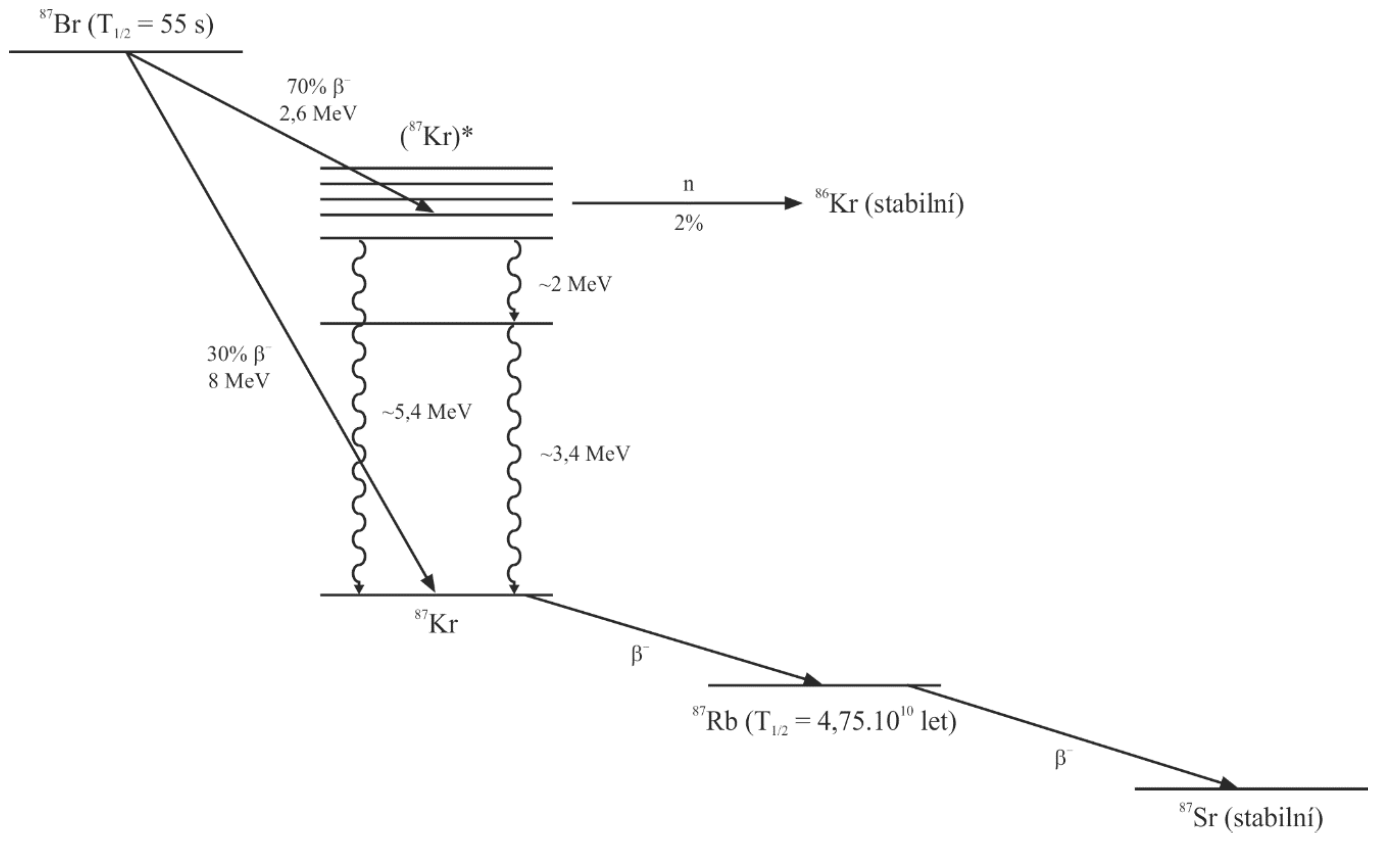
\includegraphics[width=0.8\textwidth]{img/ZpožděnéNeutrony.png}
    \caption{Rozpadové schéma $^{87}$Br.}
    \label{SNM}
\end{figure}

V současnosti bylo identifikováno téměř 400 prekurzorů zpožděných neutronů. Nejdéle žijícími jsou $^{91}\text{Rb}$ a $^{87}\text{Br}$ s poločasem rozpadu 58,4~s, respektive 55,6~s, zatímco $^{102}\text{Rb}$ a $^{101}\text{Rb}$ jsou krátkodobě žijící prekurzory s poločasem rozpadu 37~ms, respektive 32~ms. Jelikož k emisi neutronu dochází bezprostředně po rozpadu prekurzoru, řídí se časové zpoždění, s nímž se emitované neutrony objevují, zákony radioaktivního rozpadu těchto jader.

Jelikož prekurzorů je moc, tak se pro optimalizaci výpočtů prekurzory slučují do několika skupin, přičemž každá skupina je charakteristická jedním středním poločasem rozpadu a jedním společným kumulativním výtěžkem. Čím více skupin, tím přesnější výpočet, ale tím složitější a zdlouhavější výpočet. Pro první přiblížení stačí použít 1-2 skupiny, lepší kódy aplikují 6-8 skupin (záleží na knihovně, např. ENDF/B má 6 skupin a JEFF 8 skupin).

\begin{table}[H]
    \centering
    \begin{tabular}{@{}ccc@{}}
    \toprule
    Skupina & Prekurzor                              & T$_{1/2}$ (s) \\ \midrule
    1       & $^{87}$Br, $^{142}$Cs                  & 55,72         \\
    2       & $^{137}$I, $^{88}$Br                   & 22,72         \\
    3       & $^{138}$I, $^{89}$Br                   & 6,22          \\
    4       & $^{139}$I, $^{(93, 94)}$Kr, $^{143}$Xe & 2,30          \\
    5       & $^{140}$I, $^{145}$Cs                  & 0,61          \\
    6       & Br, Rb, As…                            & 0,23          \\ \bottomrule
    \end{tabular}
\end{table}

Kumulativní výtěžek označovaný jako $\beta$ se pohybuje v desetinách procenta, záleží, který izotop se štěpí. Pro $^{235}$U je to asi 0,7 \%, pro izotopy Pu je to méně. Proto jsou MOXové vsázky citlivější na změnu výkonu.

Kromě výše uvedených parametrů je důležitou charakteristikou zpožděných neutronů i jejich energie. Ta se pohybuje pro jednotlivé skupiny zpožděných neutronů v rozmezí od 200~keV do 700~keV. Porovnáme-li tento rozsah energií se střední energií okamžitých neutronů (2,2~MeV), je zřejmé, že zpožděné neutrony musí v rámci zpomalovacího procesu projít menším rozsahem energií než neutrony okamžité. Je nižší pravděpodobnost, že dojde k jejich ztrátě v důsledku úniku nebo parazitické absorpce, než v případě okamžitých neutronů. Naopak u okamžitých neutronů je vyšší pravděpodobnost, že vyvolají štěpení ve vyšší oblasti energií (např. na $^{238}\text{U}$). Tyto dva efekty mají tendenci působit navzájem proti sobě, nicméně je obvykle mezi nimi určitý, i když mírný, rozdíl. V důsledku toho se definuje tzv. efektivní podíl zpožděných neutronů $\beta_\text{ef}$, který zohledňuje rozdílnou energii zpožděných neutronů oproti neutronům okamžitým a tím i jejich význam v procesu štěpení. Je tedy závislý na typu reaktoru, moderaci apod.

\subsubsection{Emise zpožděných neutronů}

Emise zpožděných neutronů je spojena se vznikem a aktivitou jejich jednotlivých mateřských jader. Vznik konkrétního prekurzoru zpožděných neutronů v průběhu ozařování můžeme popsat bilanční rovnicí ve tvaru:

\[
\frac{dN_i}{dt} = Y_C \cdot \Sigma_f \cdot \Phi - \lambda_i \cdot N_i
\]

kde:

\begin{itemize}%[noitemsep]
    \item[$-$] $N_i$ je počet mateřských jader zpožděných neutronů $i$-tého druhu,
    \item[$-$] $Y_C$ je kumulativní výtěžek mateřských jader zpožděných neutronů ze štěpení,
    \item[$-$] $\Sigma_f$ je reakční rychlost pro štěpení,
    \item[$-$] $\Phi$ je hustota toku neutronů,
    \item[$-$] $\lambda_i$ je rozpadová konstanta mateřských jader zpožděných neutronů.
\end{itemize}

Pro jednoduchost je zanedbán záchyt neutronů mateřskými jádry zpožděných neutronů. Tuto rovnici lze jednoduše řešit pro $N_i$ jako funkci času ozařování:

\[
N_i(t) = \frac{Y_C \cdot \Sigma_f \cdot \Phi}{\lambda_i} \cdot \left(1 - e^{-\lambda_i t}\right).
\]

Abychom získali emisi zpožděných neutronů (tj. zdrojový člen), je nutné vynásobit obě strany rozpadovou konstantou $\lambda_i$. Za předpokladu, že mateřské jádro prochází rozpadem vedoucím k emisi neutronu $P_i$, předpokládáme-li, že druhů mateřských jader a ozářovacích časů je $t_\text{irr}$, pak počet zpožděných neutronů emitovaných v čase $t$ po ukončení ozařování bude:

\[
N_{DN}(t) = \sum_{i=1}^{m} P_i \cdot Y_C \cdot \Sigma_f \cdot \Phi \cdot (1 - e^{-\lambda_i t_\text{irr}}) \cdot e^{-\lambda_i t}.
\]

V souladu s teorií lze zpožděné neutrony rozdělit do šesti skupin podle typických mateřských jader a vztah přepsat na tvar:

\[
N_{DN}(t) = \sum_{i=1}^{6} a_i \cdot (1 - e^{-\lambda_i t_\text{irr}}) \cdot e^{-\lambda_i t},
\]

kde $a_i$ je zastoupení $i$-té skupiny zpožděných neutronů. Bude-li provedeno pouze krátkodobé ozařování (např. neutronovým pulzem), pak rovnice nabývá tvar:

\begin{equation}
    \boxed{N_{DN}(t) = \sum_{i=1}^{6} a_i \cdot e^{-\lambda_i t}.}
\end{equation}

Je-li doba ozařování dostatečně dlouhá ($t_\text{irr} \gg \tau_i$), přechází rovnice na tvar:

\begin{equation}
    \boxed{N_{DN}(t) = \sum_{i=1}^{6} a_i \cdot (1 - e^{-\lambda_i t}).}
\end{equation}

\subsubsection{Stanovení poločasu rozpadu prekurzorů zpožděných neutronů}

V případě, že bychom chtěli určit parametry jednotlivých skupin zpožděných neutronů a celkovou emisi rozdělit na individuální rozpadové křivky, je nutné aplikovat na analyzovaná data metody nelineární regrese. Takováto úloha není jednoduchá a pro její řešení jsou běžně používány sofistikované softwarové nástroje pro analýzu dat. Nicméně úloha se výrazně zjednoduší, pokud se bude jednat o hledání parametrů pouze jedné exponenciální funkce. Toho lze dosáhnout, pokud si uvědomíme, že platí $\lambda_1 \ll \lambda_2 \ll \dots \ll \lambda_6$ a $e^{-\lambda_1 t} \gg e^{-\lambda_2 t} \gg \dots \gg e^{-\lambda_6 t}$. Po dostatečně dlouhé době, která vede k rozpadu předchozích skupin zpožděných neutronů, můžeme vztah aproximovat pouze jednou exponenciální funkcí odpovídající nejdéle žijící skupině zpožděných neutronů:

\[
N_{DN}(t) = a_1 \cdot e^{-\lambda_1 t}
\]

Tuto funkci lze linearizovat použitím přirozeného logaritmu:

\[
\ln N_{DN}(t) = \ln a_1 - \lambda_1 \cdot t
\]

díky čemuž můžeme jednoduše určit parametry $a_1$ a $\lambda_1$. Takto získanou teoretickou emisi odečteme od celkové emise:

\[
N_{DN}(t) - a_1 \cdot e^{-\lambda_1 t}
\]

Tento rozdíl pak představuje četnost emise pro zbývající skupiny zpožděných neutronů (2 až 6), z něhož můžeme na základě výše popsané úvahy určit parametry zpožděných neutronů druhé skupiny ($a_2$ a $\lambda_2$). Tímto způsobem bychom pokračovali až k určení parametrů skupiny zpožděných neutronů s nejkratší dobou života ($a_6$ a $\lambda_6$).

Problém nastane u krátkodobých skupin (5 a 6), jelikož jejich poločas rozpadu je tak malý, že než dojde k měření, tak se většina prekurzorů rozpadne.

\subsubsection{Určování množství štěpného materiálu}

Z předchozí teorie je zřejmé, že celkový počet zpožděných neutronů emitovaných ozářeným štěpným materiálem závisí na počtu štěpení, což je samozřejmě spjato s množstvím jader ve štěpném materiálu. Tudíž lze využít této závislosti k určení vybraných vlastností zkoumaného vzorku, jako je množství, respektive obohacení štěpného materiálu ve vzorku.

Metoda určování množství nebo obsahu štěpného materiálu ve zkoumaném vzorku na základě detekce zpožděných neutronů je rychlá, nedestruktivní, přesná a velmi citlivá analytická metoda. Je založena na ozáření vzorku obsahujícího štěpný materiál neutrony a následné detekci zpožděných neutronů, které jsou emitovány tímto vzorkem. Množství nebo obsah štěpného materiálu ve zkoumaném vzorku je pak určená na základě porovnání intenzity zpožděných neutronů emitovaných tímto vzorkem se vzorky (standardy), u nichž je známo množství nebo obsah štěpného materiálu (za pomoci trojčlenky).

Předpokládejme zjednodušeně, že celkový počet zpožděných neutronů emitovaných ozářeným vzorkem a detekovaný detekčním systémem je roven součtu četností získaných za dobu detekce $(t_\text{end} - t_\text{start})$. Pak lze počet zpožděných neutronů $N_X$ odpovídající neznámému vzorku a počet zpožděných neutronů $N_\text{ST}$ odpovídající standardu, určit na základě následujících vztahů:

\[
N_X = \sum_{i = t_\text{start}}^{t_\text{end}} CR_{X,i}, \quad N_\text{ST} = \sum_{i = t_\text{start}}^{t_\text{end}} CR_{\text{ST},i},
\]

kde $CR_{X,i}$ a $CR_{\text{ST},i}$ jsou četnosti získané v $i$-tém časovém kroku detekčního systému pro neznámý vzorek a standard.

Je-li odezva detekčního systému na pozadí rovna:

\[
N_\text{BG} = \sum_{i = t_\text{start}}^{t_\text{end}} CR_{\text{BG},i},
\]

pak platí pro závislost počtu zpožděných neutronů produkovaných standardem na jeho hmotnosti $m_\text{ST}$ následující úměra:

\begin{equation}
m_X = m_{ST} \cdot \frac{N_X - N_\text{BG}}{N_{ST}-N_\text{BG}}.
\end{equation}

Přesnější výslednou hodnotu $m_X$ neznámého vzorku získáme, pokud použijeme více než jeden standard se štěpným materiálem. V takovém případě je vhodné vynést do grafu závislost celkového počtu zpožděných neutronů na množství štěpného materiálu, proložit data vhodnou křivkou a získat její rovnici. Z rovnice lze pak určit neznámé množství štěpného materiálu ve zkoumaném vzorku. Nicméně je důležité, aby se všemi vzorky bylo nakládáno za stejných experimentálních podmínek (hustota toku neutronů, doba ozařování, doba transportu vzorku a doba detekce) a kromě toho musí mít vzorky podobnou geometrii.
\section[Režimy a provoz neutronových detektorů]{Základní dělení, charakteristiky, provozní režimy a konfigurace provozních parametrů detektorů neutronů}

\subsection{Princip detekce neutronů}

Neutron je elektricky neutrální, proto pokud ho chceme detekovat, musíme postupovat nepřímo. Je potřeba neutron konvertovat na jinou nabitou částici (elektron, alfa, proton, ...), která se potom snáze detekuje. 

Detekce prostřednictvím sekundárních částic. Používají se detektory nabitých částic s konverzním materiálem naneseným na povrchu detektoru, někdy je konvertor přímo v aktivní části detektoru jako plyn, aby vznikající sekundární ionizující záření mohlo být bezprostředně detekováno. 

\subsubsection{Konvertor neutronů}

Konvertory neutronů představují klíčovou součást detektorů určených k měření neutronového záření. Jejich návrh a konstrukce musí splňovat následující požadavky.

\textbf{Požadavky na konvertor neutronů:}

\begin{itemize}
    \item \textbf{Velký účinný průřez:} Materiál použitý v konvertoru musí mít co největší účinný průřez pro jadernou reakci, při níž dochází ke konverzi neutronu.
    \item  \textbf{Dostupnost materiálu:} Nuklid použitý jako terč by měl být dostatečně zastoupen v přírodním izotopickém složení, nebo musí existovat cenově efektivní a účinný způsob získávání obohaceného materiálu.
    \item  \textbf{Energie uvolněná při reakci (Q-hodnota):} Energie uvolněná při konverzní jaderné reakci (Q) je důležitým parametrem. Vyšší hodnota Q umožňuje snazší potlačení doprovodného gama záření.
\end{itemize}

\textbf{Požadavky na konstrukci detektoru:}

Detektor musí být navržen tak, aby částice vzniklé při konverzní reakci odevzdaly celou svou kinetickou energii v jeho aktivním objemu. Aktivní délka detektoru musí být proto dostatečná, aby zajistila kompletní absorpci energie.

\textbf{Typy konvertorů podle skupenství:}

\begin{itemize}
    \item  \textbf{Plynné konvertory:} Ionizační a proporcionální plynové komory využívající plynný konvertor ($^3$He, $^{10}$BF$_3$).
    \item  \textbf{Kapalné konvertory:} Kapalné scintilátory.
    \item \textbf{Pevné konvertory:} 
    \begin{itemize}
        \item  Plynové komory s pevným konvertorem (např. s vrstvou $^{10}\text{B}$, $^{235}$U).
        \item  Scintilátory ($^6$LiI(Eu)).
        \item  Polovodičové detektory (konvertor nanesený nad PN přechodem).
        \item  Termoluminiscenční detektory (z $^6$LiF, dochází k excitaci elektronů, které zamrznou v mřížce. Po následném ohřátí se uvolní a změří).
        \item  Plastové nebo emulzní detektory zaznamenávající stopy neutronů.
    \end{itemize}
\end{itemize}

Citlivost detektoru závisí na hustotě atomů v konvertoru (počet atomů na $\text{cm}^3$). Vyšší hustota atomů zvyšuje citlivost na neutrony, avšak zároveň i na gama záření. Proto nelze jednoznačně preferovat konkrétní skupenství materiálu konvertoru; volba závisí na specifických požadavcích konkrétní aplikace.

Většina detektorů má on-line odezvu, ale existují i detektory, které se musí později vyhodnotit (TLD, aktivační fólie). Účel měření neutronů může být:

\begin{itemize}
    \item fluence neutronů (neutronový tok),
    \item spektrometrie neutronů (mimo počtu částic zaznamenáváme i jejich energie),
    \item měření ekvivalentní dávky (dozimetry).
\end{itemize}
  
Nejčastější reakce pro konverzi neutronu na nabitou částici jsou:

\[
^3\text{He} + ^1\text{n} \to ^3\text{H} + ^1\text{p} + 0{,}765 \, \text{MeV} \ \ \text{(He detektor)}
\]
\[
^{10}\text{B} + ^1\text{n} \to ^7\text{Li} + \alpha + 2{,}3 \, \text{MeV} \ \ \text{(B detektor, scintilátor)}
\]
\[
^{10}\text{B} + ^1\text{n} \to ^7\text{Li} + \alpha + 2{,}8 \, \text{MeV} \ \ \text{(B detektor, scintilátor)}
\]
\[
^6\text{Li} + ^1\text{n} \to ^3\text{H} + \alpha + 4{,}79 \, \text{MeV}  \ \ \text{(Scintilátor)}
\]
\[
^{235}\text{U} + ^1\text{n} \to \text{FP} + 195 \, \text{MeV}  \ \ \text{(štěpné komory)}
\]

%Pro detekci sekundárních nabitých částic se používají plynové, scintilační, polovodičové a další detektory. Konvertorem je helium a bór v plynné fázi, resp. bór a lithium (Li) v pevné fázi. Největší problém detektorů neutronů je "odfiltrování" doprovodných jevů (zejména doprovodného $\gamma$).


Základem nastavení jak plynových, tak scintilačních detektorů je kombinace vysokého napětí (zesílení ve fotonásobiči) a zesílení (v zesilovači), tak aby výsledné pulsy měly amplitudu vhodnou pro další zpracování. Dále je nutno nastavit diskriminaci, tak aby optimálně splňovala následující kombinaci požadavků:

\begin{itemize}
    \item Malá změna (nestabilita) vysokého napětí by měla mít za následek minimální změnu četnosti pulsů. Tzn. nastavení v oblasti lokálního minima nebo aspoň ploché části amplitudového spektra.
    \item Pulsy iniciované neutrony by měly být minimálně potlačeny (nesnižovat citlivost).
    \item Maximálně by měly být potlačeny pulsy iniciované $\gamma$ zářením.
\end{itemize}

Diskriminace se stanovuje z amplitudového spektra, které je spolu s voltampérovou charakteristikou základními charakteristikami detekčního řetězce.

Důležitým parametrem detektoru je citlivost; ta určuje jeho použitelnost v praxi. Citlivostí detektoru rozumíme podíl četností na konci detekčního řetězce a toku neutronů. Citlivost záleží na spektru neutronů a k její stanovení je potřeba stanovit absolutní hustotu toku, tak spektrum neutronů. 

\subsection{Základní dělení}
Tohle jsou tak nějak všechny možné detektory neutronů, co jsem byl schopen najít:
\begin{itemize}
    \item Plynové detektory
    \item Scintilátory
    \item Polovodičové detektory
%    \item Diamantové detektory
    \item Samonapájecí detektory (SPD)
    \item Termoluminiscenční detektory (TLD)
    \item Aktivační detektory
%    \item Detektory stop v pevné fázi
\end{itemize}

\subsubsection{Plynem plněné detektory}

Plynem plněné detektory patří k nejrozšířenějším detektorům ionizujícího záření. Měří ionizaci produkovanou průchodem nabité částice prostředím. Jsou založeny na sběru iontů a elektronů vytvořených dopadajícím zářením v prostoru detektoru. Ionizace je způsobena buď přímo ionizujícím zářením ($\alpha$, $\beta$), nebo interakcí nepřímo ionizujícího záření (elektromagnetické, neutrony) s materiálem detektoru.

Plynové detektory měřící neutrony mají stejné uspořádání jako pro nabité částice. 
Konvertor je nuklid s vysokým účinným průřezem pro neutrony (nejčastěji $^1$H, $^3$He, $^6$Li, $^{10}$B, $^{235}$U). Nejčastěji je obsažen v plynové náplni nebo materiálu pokrývajícím stěny detektoru. Plynové detektory pracují nejčastěji v režimu ionizační komory nebo proporcionality.

Plynné prostředí plynové detektoru je řídké, což je výhoda z hlediska nízké citlivost ke $\gamma$ záření, ale na druhou stranu celková nižší účinnost kvůli menšímu účinnému průřezu.

\textbf{Borové komory:}

Borové komory využívají reakci $^{10}\text{B}(n, \alpha)$. Bór může být buď nanesený na vnitřní straně stěny komory, nebo použit jako plynová náplň BF$_3$. 

Reakce probíhají dle následujících rovnic:
\[
^{10}_5\text{B} + ^1_0\text{n} \rightarrow ^7_3\text{Li} + ^4_2\alpha \quad Q = 2{,}790\,\text{MeV} \quad (6\%)
\]
\[
^{10}_5\text{B} + ^1_0\text{n} \rightarrow ^7_3\text{Li}^* + ^4_2\alpha + \gamma(0{,}48\,\text{MeV}) \quad Q = 2{,}310\,\text{MeV} \quad (94\%)
\]

Příklady borových komor: SNM10, SNM12, používané například na reaktoru VR-1.

\textbf{Lithiové, heliové a gadoliniové komory}

Lithiové komory využívají reakci $^6\text{Li}(n, \alpha)$:
\[
^6_3\text{Li} + ^1_0\text{n} \rightarrow ^3_1\text{H} + ^4_2\alpha \quad Q = 4{,}784\,\text{MeV}
\]

Heliové komory pracují na základě reakce $^3\text{He}(n, p)$:
\[
^3_2\text{He} + ^1_0\text{n} \rightarrow ^3_1\text{H} + ^1_1\text{p} \quad Q = 0{,}764\,\text{MeV}
\]

Gadoliniové komory využívají reakce $^{157}\text{Gd}(n, \gamma)$ a vyznačují se velmi vysokou citlivostí. Pro jejich správnou funkci je nutná diskriminace gama záření.

\textbf{Štěpné komory:}

Štěpné komory pracují na základě štěpných reakcí s izotopy $^{235}\text{U}$, $^{233}\text{U}$ a $^{239}\text{Pu}$:
\[
^{235}\text{U}, ^{233}\text{U}, ^{239}\text{Pu} (n, f)
\]

Na povrchu štěpné komory je štěpný materiál, jako je $^{235}\text{U}$, $^{233}\text{U}$ nebo $^{239}\text{Pu}$, což je vhodné pro detekci tepelných neutronů. Štěpitelné materiály jako $^{238}\text{U}$ a $^{232}\text{Th}$ se používají pro detekci rychlých neutronů.

Je nutné diskriminovat vliv $\alpha$ záření ze štěpných nebo štěpitelných materiálů. Štěpné komory jsou citlivé také na gama záření, což vyžaduje další diskriminaci.

Příklad použití: Štěpné komory RJ1300 na reaktoru VR-1. Tyto komory zahrnují i miniaturizované varianty s průměrem jen 4,7 mm, které jsou vhodné pro vnitro-reaktorová měření (in-core měření).

\textbf{Klasifikace plynových detektorů}

\begin{figure}[H] 
    \centering
    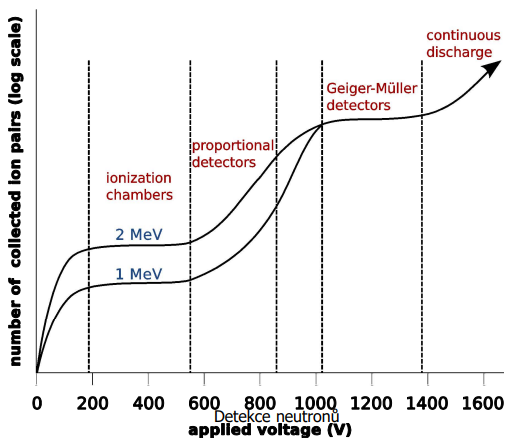
\includegraphics[width=0.5\textwidth]{img/KlasifikacePlynovýchDetektorů.png}
    \caption{Klasifikace plynových detektorů.}
    \label{fig:KlasifikacePlynovýchDetektorů}
\end{figure}

Klasifikace plynových detektorů zahrnuje několik typů, z nichž každý má své specifické vlastnosti a použití.

Ionizační komory pracují tak, že volba napětí zajistí, aby proud komorou nezávisel na napětí (nasycený proud). Odezva komory závisí i na energii záření a může být provozována impulzně i proudově.

Proporcionální detektory využívají vyšší napětí, které zvyšuje pravděpodobnost sekundární ionizace, plynového násobení a vzniku lavinového efektu. Počet iontových párů zde závisí na napětí, přičemž odezva je úměrná energii záření. Tento typ detektorů se využívá pro spektrometrii záření.

Oblast limitované proporcionality nastává při ještě vyšším napětí, které způsobí hromadění iontů u katody, což ovlivňuje elektrické pole v detektoru. Elektrony se snáze pohybují k anodě než těžké ionty ke katodě, což vytváří nelineární efekt, kdy výstupní signál není proporcionální k deponované energii. Tato oblast se dle literatury běžně nepoužívá.

Geiger-Müllerovy detektory fungují tak, že ionizující záření proniká okénkem do trubice, kde ionizuje plyn. Uvolněné elektrony jsou urychlovány k anodě, zatímco kladné ionty směřují ke katodě. Následná lavinová ionizace vede k vzniku volných nosičů náboje. Tento proces převyšuje rekombinaci, což umožňuje vznik výboje. Použití zhášedla (např. etylen, halogen) omezuje trvání výboje na mikrosekundy, což umožňuje detekci impulzů v rozsahu $10^4$ až $10^5$ za sekundu.

Koronové detektory nejsou schopny registrovat záření s nízkou ionizační schopností, jako je záření $\beta$ nebo $\gamma$. Při normálním režimu je v koronové vrstvě ionizovaný plyn, který vytváří koronový proud vedoucí ke vzniku milivoltových impulsů. Silně ionizující částice, jako jsou částice $\alpha$, mohou vytvořit impulsy s amplitudou až 300~mV. Tento typ detektorů zachovává úměrnost mezi energií částice a amplitudou impulsu.

Jiskrové detektory pracují ve vzduchu při normálním tlaku. Mezi katodou a anodou je aplikováno stejnosměrné napětí několik kilovoltů. Ionizující částice, která vstoupí mezi elektrody, způsobí jiskrový výboj, který může být detekován jako impuls napětí nebo fotograficky jako jiskra. Moderní jiskrové detektory mají velmi krátké impulsy (řádově $10^{-9}$~s), což je jejich hlavní předností oproti Geiger-Müllerovým detektorům.

Každý z těchto detektorů má specifické výhody a použití, a jejich volba závisí na požadavcích konkrétní aplikace.

\subsubsection{Scintilační detektory}

Scintilační detektory představují zařízení pro detekci ionizujícího záření, které fungují na principu excitace elektronu do vyššího energetického stavu zářením. Návrat elektronu do základního stavu je doprovázen emisí světelného záblesku.

Proces detekce probíhá ve dvou krocích:

\begin{itemize}
    \item Ionizující záření je převedeno na viditelné nebo ultrafialové světlo pomocí scintilačního materiálu (krystalu). Při absorpci záření dochází k excitaci elektronů krystalu, které následně při de-excitaci emitují fotony viditelného světla.
    \item  Viditelné světlo je detekováno a převedeno na elektronický signál pomocí zařízení, jako je fotonásobič.
\end{itemize}

Používané scintilační materiály zahrnují organické látky, jako jsou naftalen a antracen, i anorganické látky, například NaI, CsI nebo BaF$_2$. Každý materiál má specifické vlastnosti, které ovlivňují citlivost a rychlost odezvy detektoru.

Fotonásobič, který je často součástí scintilačního detektoru, funguje na principu zesílení světelného signálu. Fotony dopadají na fotokatodu, kde díky fotoelektrickému jevu dochází k emisi elektronů. Tyto elektrony jsou urychlovány a jejich počet je postupně násoben na sérii elektrod zvaných dynody. Výsledkem je zesílení signálu, které umožňuje detekci jednotlivých fotonů.

Scintilační detektory se běžně nepoužívají v I\&C systémech jaderných reaktorů, avšak nacházejí široké uplatnění v jiných oblastech, jako je medicína, fyzika částic nebo dozimetrie.

\begin{figure}[H] 
    \centering
    \includegraphics[width=0.5\textwidth]{img/Scintilátor.png}
    \caption{Scintilační detektor.}
    \label{fig:Scintilační detektor}
\end{figure}

\subsubsection{Polovodičové detektory}

Podobné jako plynové detektory. Konverze neutronu na nabitou částici probíhá v konvertoru. Nízké napětí a vysoká účinnost díky menší energii potřebné na vytvoření páru elektron-díra.

Elektrotechnické zařízení pracující na principu
fotodiody zapojené v závěrném směru, výhody
jsou malá šířka zakázaného pásu a velmi dobrá
rozlišovací schopnost. Nevýhody tohoto detektoru jsou hlavně tepelný šum a nižší detekční účinnost. Nepoužívají se běžně v I\&C jaderných reaktorů.

\subsubsection{Samonapájecí detektory}

Samo-napájecí detektory (Self Powered Neutron Detectors, SPND) nebo Self Powered Detectors (SPD) patří mezi zařízení, která využívají materiály s relativně vysokým účinným průřezem pro absorpci neutronů. Tento proces vede k následnému beta nebo gama rozpadu. Nejjednodušší forma těchto detektorů funguje na principu přímého měření proudu vzniklého z beta rozpadů po záchytu neutronů. Proud je přímo úměrný množství zachycených neutronů v detekčním materiálu, což eliminuje potřebu dodatečného pracovního napětí a ospravedlňuje označení "samo-napájecí".

Další možností je využití gama záření emitovaného po záchytu neutronu. Gama záření může tvořit sekundární elektrony pomocí Comptonova efektu, fotoelektrického jevu nebo tvorbou páru. Proud těchto sekundárních elektronů pak slouží k měření hustoty neutronového toku.

Výhody těchto detektorů zahrnují nepotřebu přívodu energie, jednoduchou a robustní konstrukci, relativně malé rozměry vhodné pro vnitro-reaktorové instalace, dobrou stabilitu při působení teplot a tlaku, nízkou cenu a jednoduchou elektroniku. Mezi nevýhody patří omezený pracovní rozsah způsobený nízkou citlivostí na neutrony, citlivost proudu na změny spektra energií neutronů, nutnost kompenzace šumů pozadí a dlouhá doba odezvy na změny hustoty neutronového toku.

Samo-napájecí detektory založené na beta rozpadu mají jako základ emitor vyrobený z materiálu s vysokým účinným průřezem pro záchyt neutronů (používá se $^{51}$V $\sigma_a\approx4,9$ b nebo $^{103}$Rh $\sigma_a\approx120$ b ). Tento materiál produkuje beta aktivní radioizotopy. Ostatní části detektoru by měly mít nízký účinný průřez a minimální interakci s neutrony. Použitý izolátor musí být odolný vůči vysokým teplotám a radiaci v aktivní zóně reaktoru, a často se využívají oxidy magnesia, křemíku nebo hliníku. Kolektor bývá z nerezavějící oceli nebo inconelu. 

Výkonnost těchto detektorů je silně ovlivněna volbou emitoru, jeho účinným průřezem a poločasem rozpadu. Nevhodně zvolený průřez může způsobit nízkou citlivost nebo rychlé vyhoření detektoru. Důležitým parametrem je i dostatečná energie beta záření, aby nedocházelo k samoabsorpci v emitoru nebo izolátoru. Krátký poločas rozpadu zajišťuje rychlou odezvu na změny hustoty neutronového toku.

Mezi vhodné materiály pro emitory SPD patří rhodium a vanad. Vanad má nižší vyhoření, což umožňuje jeho použití po delší dobu, zatímco rhodium vyžaduje častější výměnu. Výstupní proud těchto detektorů je úměrný hustotě neutronového toku, ale změny v poločasu rozpadu mohou ovlivnit odezvu při velkých změnách toku.

Alternativou jsou samo-napájecí detektory využívající sekundární elektrony z gama rozpadu. Tyto detektory mají oproti beta variantám rychlejší odezvu, ačkoliv jejich citlivost bývá nižší. Používají se například kobalt nebo hafnium, které generují sekundární elektrony z gama záření s vysokou rychlostí odezvy.

\begin{figure}[H] 
    \centering
    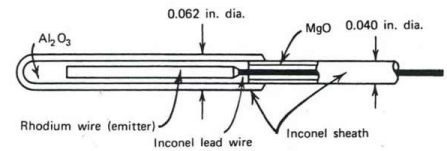
\includegraphics[width=0.5\textwidth]{img/SPD_1.png}
    \caption{Samo-napájecí detektory.}
    \label{fig:SPDKonstrukce}
\end{figure}

\subsubsection{Termoluminiscenční detektory}

Termoluminiscenční detektory jsou zařízení, která využívají schopnost některých materiálů uchovávat energii ionizujícího záření v podobě excitovaných elektronů. Když je materiál zahřátý, elektrony se uvolní z energetických pastí a při návratu na nižší energetickou hladinu vyzařují světlo.

Proces fungování termoluminiscenčních detektorů zahrnuje tyto kroky:

\begin{itemize}
    \item Ionizující záření excituje elektrony z valenčního do vodivostního pásu. Tyto elektrony jsou zachyceny v záchytných centrech.
    \item Zahřátím materiálu získají elektrony dostatečnou energii k uvolnění ze záchytných center.
    \item Při návratu do základního stavu emitují elektrony světlo, které je detekováno pomocí fotonásobiče.
\end{itemize}

Vyzařovaná energie je úměrná energii pohlceného ionizujícího záření, což umožňuje přesné měření dávky záření. 

Pro výrobu TLD se používají materiály jako lithium fluorid (LiF), calcium fluoride (CaF$_2$), magnesium beryllium oxide (MgBeO$_4$), a calcium sulfate dopovaný dysprosiem (CaSO$_4$(Dy)). Každý z těchto materiálů má různé citlivosti a energetické charakteristiky pro různé druhy záření.

Výhody termoluminiscenčních detektorů zahrnují:

\begin{itemize}
    \item Vysokou citlivost a přesnost měření.
    \item Širokou oblast lineární závislosti mezi dávkou a odezvou.
    \item Opakované použití díky možnosti vymazání zachycené energie zahřátím.
    \item Možnost použití materiálů s vlastnostmi podobnými lidské tkáni, což je výhodné pro lékařskou dozimetrie.
\end{itemize}

Nevýhody zahrnují citlivost na světlo a znečištění, což může ovlivnit přesnost měření. Termoluminiscenční detektory nejsou běžně používány v I\&C systémech jaderných reaktorů, ale nacházejí uplatnění v oblasti osobní dozimetrie.

\subsubsection{Aktivační detektory}

Aktivační detektory představují pasivní detektory ionizujícího záření, které se primárně používají k měření fluence neutronového záření. Tyto detektory mají obvykle tvar fólie nebo drátu a jsou vyrobeny buď z jednoho prvku, nebo z definované slitiny. Nejprve jsou detektory ozařovány v měřeném poli záření, během čehož dochází k indukci radionuklidů. Po ozáření se pomocí spektrometrie gama záření stanoví aktivity příslušných radionuklidů, což umožňuje výpočet celkové fluence neutronů.

Jednou z hlavních výhod aktivačních detektorů je, že jejich odezva není ovlivněna gama zářením, které je obvykle přítomné v poli neutronů. Dalšími přednostmi jsou malé rozměry a odolnost, což umožňuje jejich použití v aktivních zónách jaderných reaktorů. Pro detekci tepelných neutronů se často využívají materiály jako kobalt (Co), zlato (Au) a železo (Fe), zatímco pro rychlé neutrony se používají nikl (Ni), titan (Ti) a niob (Nb).

Specifickým příkladem použití je Aeroball Measurement System (AMS), který se používá v elektrárnách KWU. Tento systém využívá kuličky o průměru 1,7 mm vyrobené z oceli obsahující 1,5 \% vanadu. Kuličky se pohybují pneumatickým systémem (dusík) a slouží k týdenní kalibraci ostatních neutronových detektorů.

\begin{figure}[H] 
    \centering
    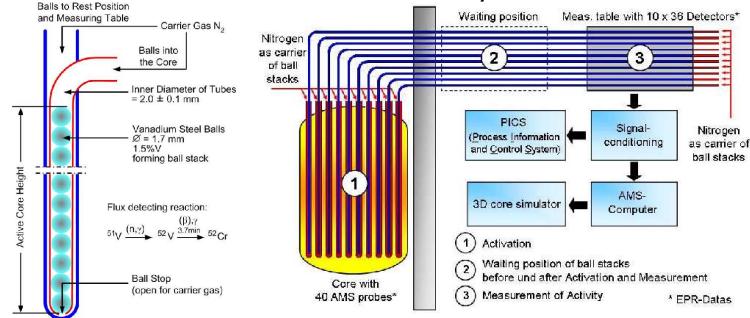
\includegraphics[width=0.5\textwidth]{img/AktivačníDetektory.png}
    \caption{Aktivační detektory v reaktoru.}
    \label{fig:AktivačníDetektory}
\end{figure}

\subsection{Charakteristiky detektorů}

\textbf{Citlivost} \textendash{} Schopnost produkovat měřitelný signál pro daný typ částic a energii. Závisí na:
\begin{itemize}
    \item účinném průřezu ionizujících interakcí,
    \item hmotnosti detektoru,
    \item šumu detektoru,
    \item tloušťce detektoru.
\end{itemize}

\textbf{Odezva} \textendash{} Vztah mezi energií částice a výstupem na detektoru (celkovým nábojem nebo amplitudou proudového pulsu).

\textbf{Funkce odezvy} \textendash{} Spektrum monoenergetického svazku je detektorem pozorováno jako komplikovaná funkce, většinou blízká Gaussově funkci s chvostem k nižším energiím.

\textbf{Mrtvá doba} \textendash{} Doba potřebná pro vytvoření a zpracování signálu v detektoru. Velmi vysoká mrtvá doba vede k navrstvení pulzů přes sebe, což následně způsobuje spektrální posun a horší rozlišení.

\textbf{Detekční účinnost} \textendash{} Poměr mezi počtem částic vyzářených zdrojem a detekovaných detektorem (absolutní účinnost). Ta se skládá z:
\begin{itemize}
    \item vnitřní účinnosti,
    \item geometrické účinnosti (akceptance).
\end{itemize}

\textbf{Energetické rozlišení} \textendash{} Nejmenší rozlišitelný rozdíl energie $\Delta E$ mezi dvěma blízkými energiemi. U monoenergetického svazku je ideálně $\delta$-funkce, reálně pík s konečnou šířkou (většinou Gaussův tvar). Rozlišení se udává ve formě pološířky (FWHM) jako relativní rozlišení $\Delta E / E$ v \%.

\textbf{Časové rozlišení} \textendash{} Nejmenší rozlišitelný rozdíl časů, definice podobná jako u energie.

\textbf{Dráhové rozlišení} \textendash{} Nejmenší rozlišitelný rozdíl v dráze, definice obdobná jako u předchozích veličin.

\subsubsection{Parametry detektorů neutronů}

\textbf{Citlivost k neutronům} \textendash{} Závisí na:
\begin{itemize}
    \item účinném průřezu konverzního materiálu a energii neutronů,
    \item objemu a hustotě detektoru (absorpce náboje).
\end{itemize}

\textbf{Energie reakce} \textendash{} Energie uvolněná záchytem neutronu ($Q$-energie), která determinuje kinetickou energii detekovatelné částice.

\textbf{Potlačení $\gamma$ záření} \textendash{} "Průhlednost" detektoru pro $\gamma$ záření v porovnání s velikostí $Q$:
\begin{itemize}
    \item větší $Q$ zajišťuje lepší odstup od šumu a $\gamma$ záření,
    \item "průhlednost" detektoru pro $\gamma$ závisí na hustotě a $Z$ detektoru.
\end{itemize}

\textbf{Možnost získání informace o energii původního neutronu} \textendash{} Kolekce celého vzniklého náboje zajišťuje spolehlivou diskriminaci a umožňuje spektroskopii. Používají se například:
\begin{itemize}
    \item konverze (n, $\alpha$),
    \item metoda odražených protonů.
\end{itemize}

\begin{table}[h!]
\centering
\caption{Parametry a jejich význam v kontextu detekce neutronů.}
\label{tab:parameters}
\resizebox{\columnwidth}{!}{
\begin{tabular}{cc}
\toprule
\textbf{Parameter}               & \textbf{Význam}                                                                                   \\ \midrule
$\Phi$ (fluence)                 & Tok neutronů (počet neutronů na jednotku plochy)                                                  \\ 
$\sigma$ (cross-section)         & Účinný průřez (pravděpodobnost interakce neutronů s látkou)                                        \\ 
$R$ (reaction rate)              & Rychlost reakcí (počet reakcí za sekundu)                                                         \\ 
$E$ (energy)                     & Energie neutronů                                                                                  \\ 
$dE/dx$ (stopping power)         & Ztráta energie na jednotku délky při průchodu částic prostředím                                   \\ 
$L$ (mean free path)             & Střední volná dráha (průměrná vzdálenost mezi interakcemi neutronů s látkou)                      \\ 
$\epsilon$ (detector efficiency) & Detekční účinnost (podíl registrovaných interakcí vůči celkovému počtu interakcí)                  \\ 
$\Delta E$ (energy resolution)   & Energetické rozlišení (schopnost detektoru rozlišit různé energie částic)                         \\ 
$T$ (time resolution)            & Časové rozlišení (schopnost detektoru rozlišit události v čase)                                   \\ 
$S/N$ (signal-to-noise ratio)    & Poměr signálu k šumu (kvalita měřeného signálu vůči šumu pozadí)                                  \\ \bottomrule
\end{tabular}
}
\end{table}

\subsection{Provozní režimy a konfigurace provozních parametrů}

\subsubsection*{Impulsní režim komory}

V impulzním režimu komory se detekují jednotlivé impulzy z neutronové komory. Signál je následně zesílen a diskriminován. Diskriminace slouží k tomu, aby byla zvýrazněna odezva na neutrony, která je nejsilnější, a naopak potlačeny impulzy s menší amplitudou, jako jsou impulzy způsobené gama, beta, alfa zářením nebo šumem. Tyto složky jsou eliminovány diskriminací. V tomto režimu je však třeba řešit problematiku mrtvé doby. Maximální četnost impulzů bývá typicky do 10$^5$ impulzů za sekundu, přičemž na zařízení VR-1 dosahuje přibližně $5 \cdot10^4$ impulzů za sekundu. Při vysokých četnostech impulzů může nastat problém stejnosměrného posunu signálu za kondenzátorem, což lze kompenzovat pomocí speciálních systémů, například systému dataPartner pro reaktor LVR-15.


\subsubsection*{Proudový režim komory}
V proudovém režimu komory se měří celkový stejnosměrný proud (DC) protékající komorou. Tento režim umožňuje potlačit mrtvou dobu, což je výhodné zejména při měření velkých hustot neutronového toku. Na druhé straně zde není možné využít standardní diskriminaci k potlačení vlivu alfa a gama záření či šumu. Proudový režim se používá pro velké rozsahy proudů, kde je vhodné využít logaritmické zesilovače nebo Campbellovu metodu, která vychází ze vztahu $n=\text{RMS}^2$. Pro potlačení vlivu gama záření se využívají kompenzované komory nebo Campbellovský režim.

\textbf{Kompenzovaná komora:}

Kompenzovaná komora se skládá ze dvou částí. První část měří jak neutrony, tak gama záření, zatímco druhá část měří pouze gama záření. Pro získání čistého signálu neutronů se odečítají proudy z obou částí podle vztahu $I_n=I_{\gamma+n}-I_{\gamma}$. Tento přístup umožňuje eliminovat vliv gama záření a získat přesné údaje o neutronovém toku

\begin{figure}[H] 
    \centering
    \includegraphics[width=0.5\textwidth]{img/KompenzovanáKomora.png}
    \caption{Kompenzovaná komora.}
    \label{fig:KompenzovanáKomora}
\end{figure}


\textbf{Campbellovský režim:}

Proudový režim, který využívá jen střídavou
složku (AC) proudu.

Campbellova metoda přináší několik významných výhod, které ji činí atraktivní pro aplikace v detekci záření. Především využití střídavých (AC) zesilovačů, které se snáze konstruují a nabízejí lepší stabilitu a menší drift ve srovnání se stejnosměrnými (DC) zesilovači.

Další výhodou je kvadratická závislost výkonu na RMS (Root Mean Square), která umožňuje pokrýt celý výkonový rozsah typicky pouze jedním měřicím kanálem.

Navíc Campbellova metoda poskytuje velmi dobrou diskriminaci gama záření, která je srovnatelná s diskriminací dosažitelnou pomocí kompenzovaných komor.

\textcolor{red}{CHYBÍ KONFIGURACE PROVOZNÍCH PARAMETRŮ!!!} 



\section[Neutronové zdroje]{Měření základních charakteristik radionuklidových, generátorových a fotoneutronových zdrojů neutronů}

Něco je v přednášce 1 NAA, ale ně moc důkladně, lepší převzít z lepších materiálů.
\section[Spektrometrie neutronů]{Spektrometrie neutronů pomocí Bonnerových sfér a scintilačních detektorů na bázi odražených jader}


\section[Interakce gamma záření]{Interakce gama záření s látkou, charakteristika gama spektra, charakteristiky a kalibrace detektorů}

\subsection{Základní poznatky}

\subsubsection{Zdroje fotonů}

Hlavním zdrojem gamma fotonů je RA rozpad částic (primárně $\beta$, pro vyšší $Z$ i $\alpha$). Nově vzniklá jádra jsou nestabilní a energie se zbavují za pomoci vyzáření gamma fotonu o specifické energii a intenzitě. Tato energie je charakteristická pro daný izotop, a ačkoliv je gamma foton vyzářen nově vzniklým jádrem, v tabulkách se připisuje k původnímu nestabilnímu jádru (např. $^{90}$Sr se rozpadá na $^{90}$Y, gamma foton vyzáří $^{90}$Y, ale v tabulkách ho najdu u $^{90}$Sr). Tento proces je velmi rychlý, pokud k němu nedojde do XX sekund, tak se vzniklé izotopy označují jako \textbf{metastabilní stavy}.

Mimo to jsou s produkcí gamma fotonů spojeny další procesy související s RA rozpady:

\begin{itemize}
    \item $\beta^+$ rozpad -- vzniká pozitron, který je ihned zastaven v látce. Najde kamaráda elektron, čímž vzniká \textbf{pozitronium} (neboli krátce žijící vazba pozitronu a elektronu), anihiluje a vznikají 2 fotony o energii 511 keV jdoucí od sebe pod úhlem 180° (mohou vzniknout i 3 fotony, viz níže), tzv. \textbf{anihilační záření}. Jelikož před anihilací nezastaví pozitron uplně na nulu, je vzniklý peak rozmazaný.
    \item EC -- vzniká vakance v orbitale (nejčastěji K), která je zaplněna kaskádovými přeskoky z vyšších orbitalů, čímž vzniká charakteristické \textbf{RTG záření} (nebo Augerův elektron).
    \item IC -- neboli vnitřní konverze, nestabilní jádra se mohou energie zbavit tak, že vnitřně předají energii elektronům v obale. Ten je uvolněn, vzniká vakance, která je opět kaskádami zaplněna za vzniku charakteristického \textbf{RTG záření} (nebo Augerova elektronu).
\end{itemize}

K tomu navíc existuje:

\begin{itemize}
    \item \textbf{okamžité záření} -- vzniká v důsledku jaderných reakcí, např. (n,$\gamma$), tedy gamma fotony uvolněné hned v rámci reakce, nikoliv následný rozpad (může přesahovat až 10 MeV).
    \item \textbf{brzdné záření} -- vzniká, pokud na nabitou částici působí zrychlení (zatáčí vlivem magnetického pole, k čemuž postačí Coulombovské pole vzbuzené jádrem), což je doprovázeno ztrátou energie ve formě brzdného záření. Záření je spojité a přispívá k nárůstu kontinua v gamma spektru. Záření je vyšší pro vyšší $Z$, proto by v oblasti detektoru měly být lehké materiály.
\end{itemize}

\subsubsection{Členění fotonů}

\begin{itemize}
    \item \textbf{RTG fotony} -- vznikají v orbitalech přeskoky elektronů. Energie je dána rozdílem energií orbitalů, což je dáno hlavním a vedlejším kvantovým číslem. Nicméně elektron nemůže skákat jen tak, řídí se Paulovým vylučovacím principem, který jasně říká, v jakém pořadí se elektrony zaplňují. Nižší energie, do desítek keV. Záření je čárové a charakteristické, ale ke každému izotopu existuje spoustu peaků, jelikož záleží na přesném módu přestupu (K$_{\alpha1}$, K$_{\alpha2}$ apod.).
    \item \textbf{Gamma fotony} -- vznikají deexcitací jádra. Opět čátové charakteristické záření, ale je zde výrazně méně možností (žádné módy). Energie je vyšší, až jednotky MeV.
    \item[-] V oblasti 1 MeV se fotony překrývají, členění není tak striktní.
\end{itemize}

\subsection{Interakce gamma záření s látkou}

Fotony jsou EM záření, kterému přísluší kvantum energie dle:

$$ E_\gamma = h \nu = h \dfrac{c}{\lambda}. $$

Vlnové délky se pohybují řádově $\lambda << 10^{-10}$ m, což je výrazně méně než meziatomové vzdálenosti v mřížce. Někdy se chová jako vlna (fotoefekt), jindy jako kulička (Comptonův rozptyl).

Jelikož nejde o nabité částice (tzv. \textbf{nepřímo ionizující záření}), tak se při detekci musí spoléhat na konverzi a detekují se až sekundární částice (elektrony).

Typ interakce je podmíněný energií (např. k tvorbě páru nedojde, je-li energie pod 1022 keV). 

\textbf{Koeficient zeslabení} = charakterizuje zeslabení způsobené absorbcí v daném materiálu (osa $y$) v závislosti na energii (osa $x$). Jde o součet křivek zeslabení způsobených fotoefektem, omptonovým rozptylem a tvorbou páru.

\textbf{Absorbční koeficient} = podíl energie pohlcené absorbčním materiálem při průchodu gamma záření, jelikož ne každá interakce vede na absorbci celé energie primárního fotonu.

\subsubsection{Primární interakce}

Máme 3 základní a nejdominantnější primární interakce: fotoefekt, Comptonův rozptyl a tvorba párů. Zbytek interakcí je z pohledu detekce zanedbatelný. Tím vznikají sekundární nabité částice (elektrony), které je možné detekovat.

Celkovou pravděpodobnost interakce (mikroskopický účinný průřez $\tau$, $\sigma$ a $\kappa$) je pak možné převést do \textbf{lineárního koeficientu zeslabení}, který vyjadřuje pravděpodobnost interakce na jednotku dráhy (makroskopický účinný průřez $\mu$). 

Z toho vychází i \textbf{střední volná dráha} $\lambda$:

$$ \lambda = \dfrac{1}{\mu}, $$

a \textbf{zeslabovací zákon}:

$$ \boxed{ \dfrac{I(x)}{I_0} = e^{-\mu x}. } $$

Pokud je vzorek emitující fotony tlustý (tloušťka $L$), dochází k samostnínění (část fotonů se pohltí) a celková intenzita se musí určit integrací:

$$ \boxed{ I_\gamma(L) = \dfrac{1}{L} \int_0^L I_\gamma^0 e^{-\mu x} \: \text{d}x = \dfrac{I_\gamma^0}{\mu L} \left( 1 - e^{-\mu L} \right).} $$

V tabulkách se pak uvádí \textbf{hmotnostní koeficient zeslabení}, který je svázaný s hustotou materiálu:

$$ \mu(\text{cm}^2{\text{/g}}) = \dfrac{\mu(\text{1/cm})}{\rho(\text{g/cm}^3)}. $$

\begin{figure}[H]
    \centering
    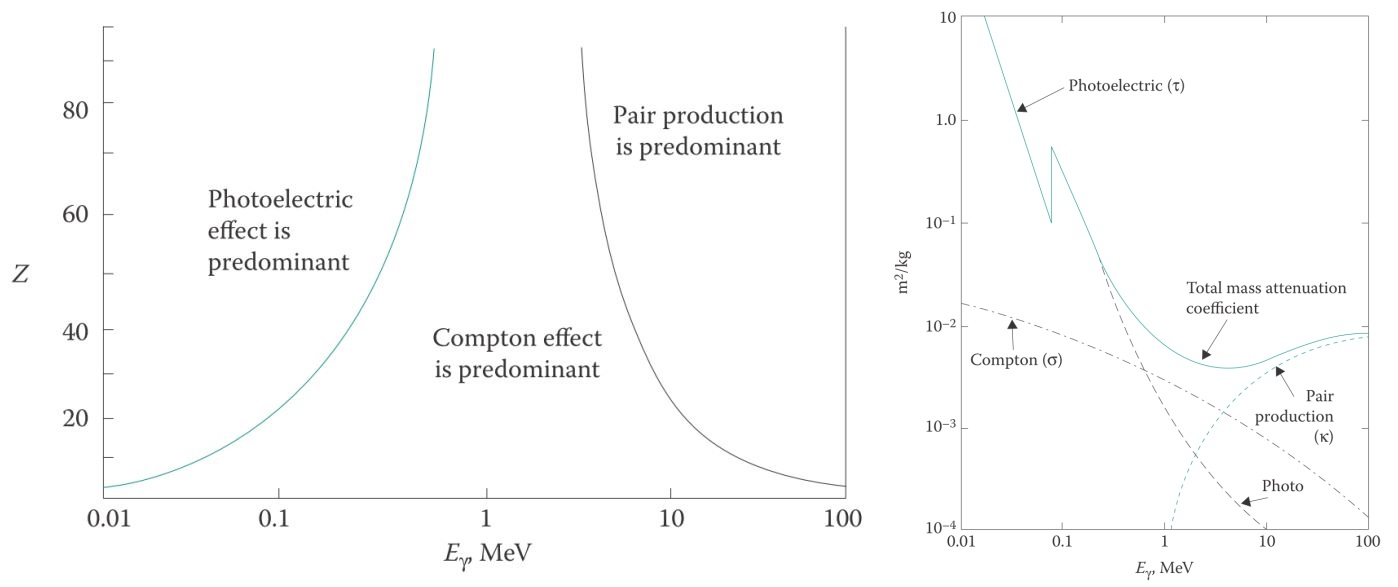
\includegraphics[width=1\textwidth]{img/interakce.JPG}
\end{figure}

\textbf{Fotoefekt:} jde o jev, kdy primární foton interaguje s elektronem v obalu, odevzdá mu veškerou svoji energii, foton zanikne a tzv. fotoelektron je uvolněn (energie fotonu $E_\gamma$ se rozdělí na vazebnou energii elektronu $E_b$ a kinetickou energii elektronu $E_e$):

$$ E_e = E_\gamma - E_b. $$

Jde o dominantní reakci při absorbci do 200 keV. Pravděpodobnost rekace (účinný průřez reakce $\tau$) klesá s energií $E_\gamma$ a roste se $Z$, jako:

$$ \tau = c \dfrac{Z^n}{E_\gamma^{3,5}}, \: \: \: n \in (4,5). $$

Energetické spektrum fotoelektronů (sekundární částice) je \textbf{čárové} a fotoefekt je zodpovědný za \textbf{peak úplného pohlcení}. Fotoelektrony mohou být uvolněny z libovolného orbitalu (nejpravděpodobněji K orbital), nicméně při nižší energii než $E_{V_K}$ už foton není schopný vyrazit elektron z K orbitalu, $\tau$ skokově klesá a dochází k vyrážení z vyšších orbitalů.

\begin{figure}[H]
    \centering
    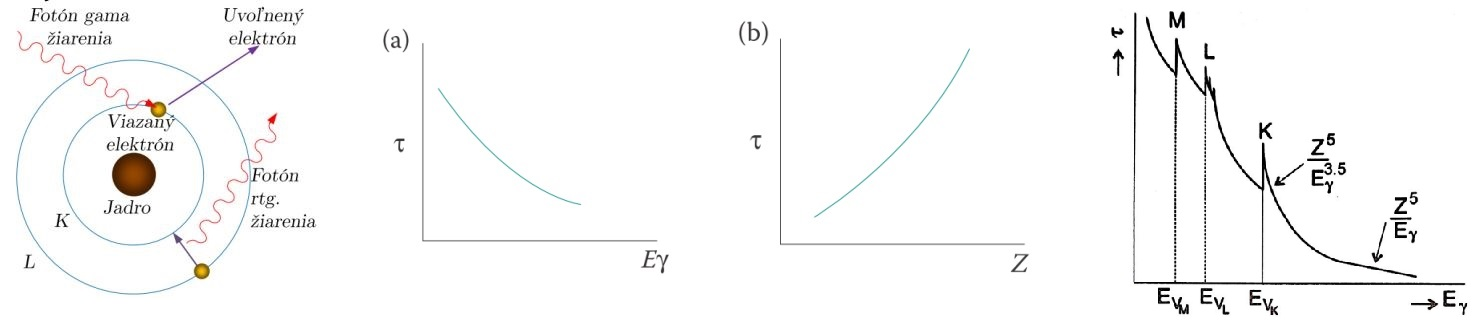
\includegraphics[width=1\textwidth]{img/fotoefekt.JPG}
\end{figure}

\textbf{Comptonův rozptyl:} jde o rozptyl fotonů na atomovém obale. Foton se odrazí od elektronu pod úhlem $\theta$ s novou energií (resp. vlnovou délkou) dle vztahu:

$$ E_\gamma' = \dfrac{E_\gamma}{1 + \dfrac{E_\gamma}{m_\text{e}c^2}(1 - \text{cos}(\theta))}. $$

Dochází k němu pro všší energie, pokud je energie nalétávajícího fotonu vyšší, než vazebná energie elektronu v obalu. Pravděpodobnost interakce (účinný průřez $\sigma$) je úměrná $Z$ a nepřímo úměrná energii $E_\gamma$:

$$ \sigma \sim \dfrac{Z}{E_\gamma}. $$

Tím vznikají odražené elektrony (sekundární částice), které jsou detekovány. Energetické spektrum odražených elektronů je \textbf{spojité}, tzv. \textbf{Comptonovo kontinuum}. To je zakončeno \textbf{Comptonovou hranou}, která je dána maximální energií elektronů (k tomu dojde, dojde-li k čelní srážce, kdy $\theta = 180°$).

Úhlová sitribuce rozptýlených fotonů je dána Klein-Nishinovým vztahem pro diferenciální účinný průřez, s rostoucí energií gamma fotonů roste pravděpodobnost dopředných úhlů.

\begin{figure}[H]
    \centering
    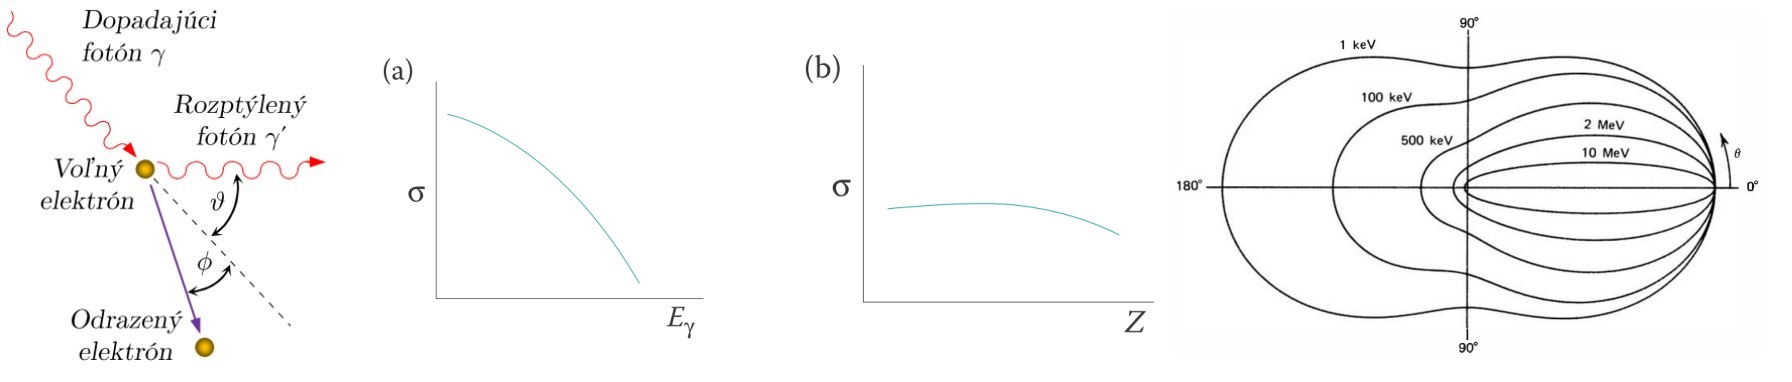
\includegraphics[width=1\textwidth]{img/Compton.JPG}
\end{figure}

\textbf{Tvorba elektron-pozitron páru:} jde o důsledek interakce gamma fotonu s jádrem. Dojde k zaniknutí gamma fotonu a vznikne pár elektron-pozitron o energiích:

$$ E = \dfrac{1}{2} (E_\gamma - 1022 \text{ keV}). $$

Elektron i pozitron se ihned zastaví a v případě pozitronu dojde ke vzniku pozitronia, anihilaci a vzniku 2-3 fotonů.

Pravděpodobnost interakce (účinný průřez $\kappa$) roste s energií $E_\gamma$ a je přímo úměrná $Z^2$. Zároveň jde o prahovou reakci a je dominantní pro vysoké energie:

$$ \kappa \sim Z^2 \: \text{ln} \left( \dfrac{E_\gamma}{m_\text{e} c^2} \right). $$

\begin{figure}[H]
    \centering
    \includegraphics[width=0.7\textwidth]{img/pár.JPG}
\end{figure}

\textbf{Fotojaderné reakce:} při interakci a pohlcení gamma fotonů může být z jádra emitován nukleon.

Jde o prahové reakce a je jich spousta: ($\gamma$,n), ($\gamma$,2n), ($\gamma$,p), ($\gamma$,np), ($\gamma$,$\alpha$) apod. Jde o prahové reakce (alespoň 5 MeV), v porovnání s předchozími 3mi reakcemi jsou zanedbatelné. Problematické v radiační ochraně (emitují se těžké nabité částice).

V JI se využívají hlavně k emitování neutronů, jako fotojaderné neutronové zdroje (např. $^{206}$Pb, $^{9}$Be, $^2$H, $^{7}$Li, $^{14}$N apod.)

\textbf{Rayligho rozptyl:} jde o koherentní rozptyl fotonu s celým obalem (tedy se všemi elektrony), přičemž nedochází k ionizaci, ani excitaci (nepřenáší se enegie, vlnová délka fotonů se zachovává). Pouze se mění směr hybnosti fotonů.

Opět nepříliš dominantní interakce, lze zanedbat. Roste pro nízké energie fotonů a vysoká $Z$. Vsuvka, vysvětluje, proč je obloha modrá (ale nevim proč :D).

\subsubsection{Druhotné efekty}

V případě detekce může docházet k zaznamenávání nechtěných druhotných efektů.

\textbf{Vícenásobná interakce:} Comptonovsky rozptýlené fotony v citlivé oblasti detektoru mohou znovu interagovat (fotoefektem, Comptonovsky), což může přispět do peaku úplné absorbce, nebo vytvořit novou Comptonovu hranu.

\textbf{Peak zpětného rozptylu:} fotony proletí detektorem bez interakce, Comptonovsky interagují až v okolním materiálu, rozptýlí se zpět s nižší energií do citlivé oblasti detektoru a jsou zaregistrovány. Tím vzniká peak zpětného rozptylu s nižší energií.

\textbf{Anihilace elektron-pozitron:} pokud mimo detektor dojde ke tvorbě páru, vzniklý elektron a pozitron za vzniku pozitronia anihilují a jeden z fotonů se dostane zpět do detektoru. Absorbcí fotoefektem vzniká anihilační peak 511 keV.

\textbf{Pozitronium} je vázaný systém, analogický atomu vodíku, kdy elektron a pozitron obíhají kolem společného těžiště s dobou života okolo 10$^{-10}$. Existují 2 typy v závislosti na spinu:

\begin{itemize}
    \item Para-pozitronium -- spiny opačně, vznikají 2 fotony o energii 511 keV (dominantní),
    \item Orto-pozitronium -- spiny shodně, vznikají 3 fotony (málo časté).
\end{itemize}

\textbf{RTG záření:} je způsobené fotoefektem, kdy je vzniklá vakance zaplněna jiným elektronem a vyzářením RTG záření.

\textbf{Augerovy elektrony:} konkurenční proces k RTG záření, pouze je přebytečná energie předána sousednímu elektronu, který je uvolněn a vyletí ven.

\textbf{Brzdné záření:} vzniká, pokud elektrony a pozitrony proletí kolem jádra, které vyvolává Coulombovo EM pole.

\textbf{Sumační efekty:} ovlivněno geometrií detektoru, můžou být zaznamenány 2 gamma kvanta ve stejný okamžik (např. 511 keV + gamma deexcitace)

\textbf{Pozadí:} detektor detekuje záření z přirozeného prostředí, jde hlavně o izotopy $^{40}$K, $^{137}$Cs a produkty rozpadových řad (urany, radony apod.). Lze zamezit dobrým stíněním.

\subsection{Charakteristika gamma spektra}

\subsubsection{Tvar gamma spektra}

Spektrum, které zaznamenám, je dáno vlastnostmi detektoru.

\textbf{Limitní případ malého detektoru:} nastává, pokud střední volná dráha sekundárních fotonů (řádově jednotky cm) je výrazně větší, než citlivá plocha detektoru (do 1-2 cm). Detektor tak zaznamená pouze primární interakce, nedochází k vícenásobné interakci. Sekundární fotony vyletí ven.

Za předpokladu, že detektor zaznamená veškerou energii sekunádrních elektronů, tak se spektrum projeví Comptonovým kontinuem zakončeným Comptonovou hranou (Comptonův rozptyl) a fotopeakem úplné absorbce (fotoefekt, vznikne \textbf{FEP = Full Energy Peak}). 

Pro energie větší než 1022 keV se navíc projeví efekt tvorby párů (vznikne \textbf{DEP = Double Escape Peak}), anihilační fotony (jde o sekundární fotony) uniknou.

$$ E_\text{DEP} = E_\text{FEP} - 2 \cdot 511 \text{ keV}. $$

\begin{figure}[H]
    \centering
    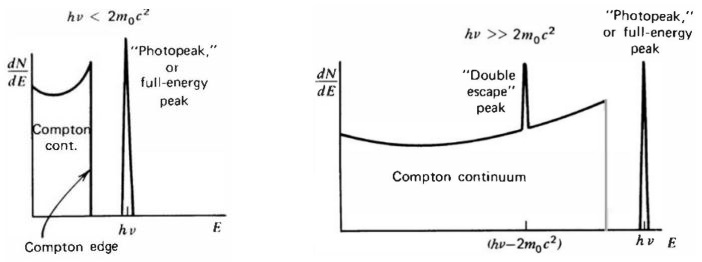
\includegraphics[width=0.7\textwidth]{img/maly_detektor.JPG}
    \caption{Tvar gamma spektra pro malý detektor ($E_\gamma < 1022$ keV vlevo, $E_\gamma > 1022$ keV vpravo).}
\end{figure}

\textbf{Limitní případ velkého detektoru:} pokud je střední volná dráha sekundárních fotonů výrazně menší, než rozměry detektoru. Ten pak zaznamená veškeré interakce, nic neunikne. Nakonec pak vždy dojde k fotoabsorbci, veškerá energie primárního záření je doponována v detektoru, tudíž zaznamenaný náboj sekundárních elektronů odpovídá energii primárního záření. Výsledná odezva je stejná, jako by primární gamma záření interagovalo pouze fotoefektem.

Spektrum se projevuje pouze peakem úplné abosrbce FEP, v tomto případě \textbf{peak úplného pohlcení}.

\begin{figure}[H]
    \centering
    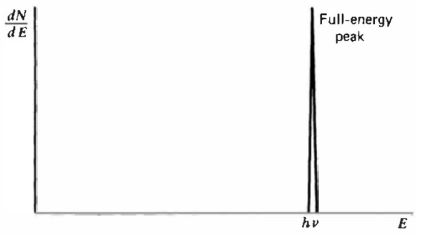
\includegraphics[width=0.4\textwidth]{img/velky_detektor.JPG}
    \caption{Tvar gamma spektra pro velký detektor.}
\end{figure}

\textbf{Středně velký detektor:} Ve skutečnosti vždy něco vylétne (kor, pokud dojde k reakci na kraji detektoru), tudíž reálný detektro zaznamená něco mezi. Nízkoenergetické záření se zaznamená lépe, jelikož nedochází tak často k sekundárním interakcím. Pak dochází k vícenásobným Comptonovým rozptylům, které vyplňují mezeru mezi Comptonovou hranou a fotopíkem.

Pro energie větší než 1022 keV se opět projevuje DEP, ale navíc i \textbf{SEP = Single Escape Peak} (pokud jeden foton unikne, a druhý ne).

$$ E_\text{SEP} = E_\text{FEP} - 511 \text{ keV}. $$

\begin{figure}[H]
    \centering
    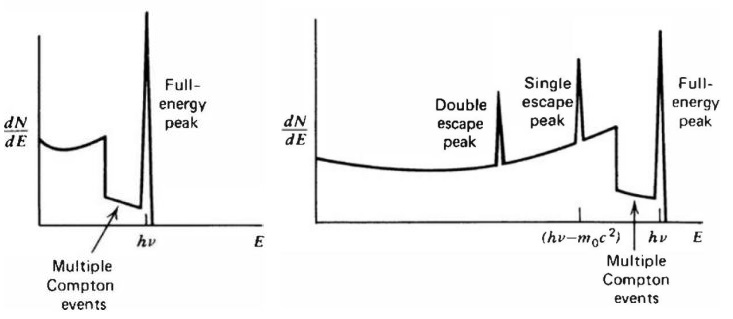
\includegraphics[width=0.7\textwidth]{img/stredni_detektor.JPG}
    \caption{Tvar gamma spektra pro středně velký detektor ($E_\gamma < 1022$ keV vlevo, $E_\gamma > 1022$ keV vpravo).}
\end{figure}

V každém případě nedojde k deponování veškeré energie a některé sekundární fotony uniknou, tento efekt nárůstá s energií těchto fotonů. To způsobuje zkreslení odezvové funkce a některé události jsou posunuty do nižších energií.

$\rightarrow$ \textbf{Ve zkratce.} Pokud mi nic neunikne, objeví se pouze FEP. Reálně ale něco unikne, což se projeví ve formě SEP a DEP (uniklé anihilační fotony). Pokud je detektor hodně malý, tak unikne vše sekundární a projeví se pouze DEP.

Ideálně chceme znát pouze FEP, přičemž Comptonovo kontinuum nám zkresluje měření. Pro jeho potlačení je možné využít koincidenční nebo antikoincidenční zapojení vícera detektorů a detekovat pouze určité interakce (v tomto případě FEP):

\begin{itemize}
    \item Comptonův spektrometr -- gamma-gamma spektrometr, mám 2 detektory pod úhlem $\theta$ a matematickým postprocessingem Comptonovo kontinuum eliminuju.
\end{itemize}

\subsubsection{Další efekty}

\textbf{RTG únikové peaky:} ty jsou způsobeny tím, že uniknou RTG fotony, které vzniknou kaskádou po fotoefektu (tzv. \textbf{XEP = X-ray Escape Peak}). V případě nekonečně velkého detektoru neuniknou a opět se veškerá energie deponuje v FEP.

$$ E_\text{XEP} = E_\text{FEP} - E_\text{X}. $$

\textbf{Anihilační peaky:} projeví se hlavně, je-li zářič $\beta^+$ radioaktivní. Pozitron anihiluje v materiálu a vzniknou gamma fotony o 511 keV. Pokud neuniknou, projeví se ve formě FEP na energii právě 511 keV. Pokud zaznamenáváme celou prostorovou geometrii, tak se projeví ve formě FEP na energii 1022 keV (zaznamenám oba dva najednou).

\textbf{Brzdné záření:} pokud máme gamma zářič $\beta$ radioaktivní, mohou unikat $\beta$ částice přímo ze zdroje a za vzniku brzdného záření zkreslovat spektrum. K tomu se používají filtry ($\beta$ absorbátory) z lehkých materiálů, které je pohltí (např. Be).

\textbf{Okolní materiály:} tvar gamma spektra a jeho zkreslení mohou ovlivňovat i okolní materiály, s kterými záření může interagovat (stínění, pouzdro, materiál zářiče, zpětně rozptýlené gamma, sumační peaky apod.)

\begin{figure}[H]
    \centering
    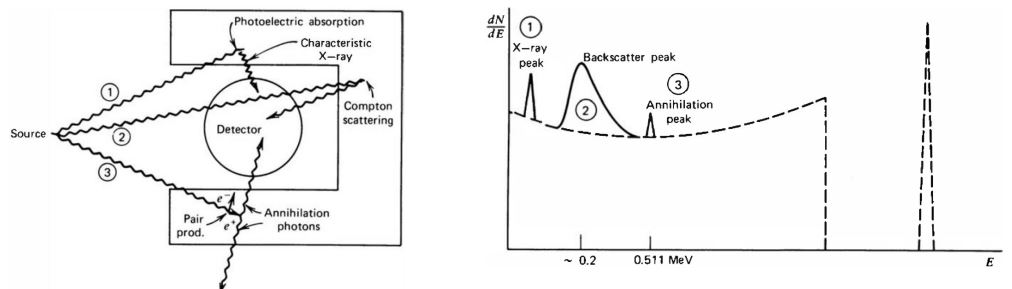
\includegraphics[width=0.9\textwidth]{img/vliv_materialu.JPG}
    \caption{Vliv okolních materiálů na tvar gamma spektra.}
\end{figure}

\subsubsection{Měření}

Při měření se projevuje statistika. My jsme v rámci detekce schopni zaznamenat histogramový záznam v jednotlivých energetických kanálech. Pod 100 zaznamenaných událostí je třeba uvažovat Poissonovo rozdělení, nad 100 událostí Gaussovo rozdělení (čas vs. aktivita). 

Ve výsledku poté zaznamenáme celkovou plochu pod peakem $S$ s potlačením Comptonova kontinua a pozadí pod peakem a s nejistotou, kterou určím z matematického popisu Gaussiánu. Dále se určí statistická významnost dle:

\begin{itemize}
    \item kritický limit $L_C$ -- plocha $S$ musí být větší než minimální hodnota,
    \item horní limit $L_U$ -- hodnota, kterou by plocha $S$ neměla překročit,
    \item detekční limit $L_D$ -- hodnota, nad kterou je plocha $S$ detekovatelná,
    \item limit stanovitelnosti $L_Q$ -- hodnota, nad kterou určím plochu $S$ s předem danou nejistotou.
\end{itemize}

$$ L_C < L_D < L_Q < S < L_U $$

\textbf{MDA} = Minimální detekovatelná aktivita, jde o nejmenší aktivitu, které může být s jistoutou měřené.

\subsection{Detektory gamma záření}

\subsubsection{Základní typy detektorů}

\textbf{Scintilační detektory:}

\begin{itemize}
    \item[1)] Primární gamma záření putuje do scintilačního krystalu, absorbuje se a část záření se transformuje na záblesk viditelného světla (\textbf{luminiscence}, atomy jsou excitovány a deexcitují viditelnými fotony), energie je úměrná světelnému signálu.
    \item[2)] Fotony putují fotonásobičem (elektronka), který mění světlo na elektrický signál. Ve formě fotokatody na vstupu, ze které jsou fotoefektem emitovány elektrony (to je ten signál).
    \item[3)] Na výstupu je anoda a vzniklé napětí urychluje elektrony za vzniku elektrického proudu. elektrony postupně dopadají na dynody, na kterých jsou vyráženy nové elektrony (2-6) a signál je zesilován. Je možné zesílit intenzitu elektronů až o 5 řádů.
    \item[4)] Takto zesílený proud je již detekovatelný, je vyveden na pracovní odpor, na kterém se mění napětí (to je ten signál, který měřím). 
\end{itemize}

\begin{figure}[H]
    \centering
    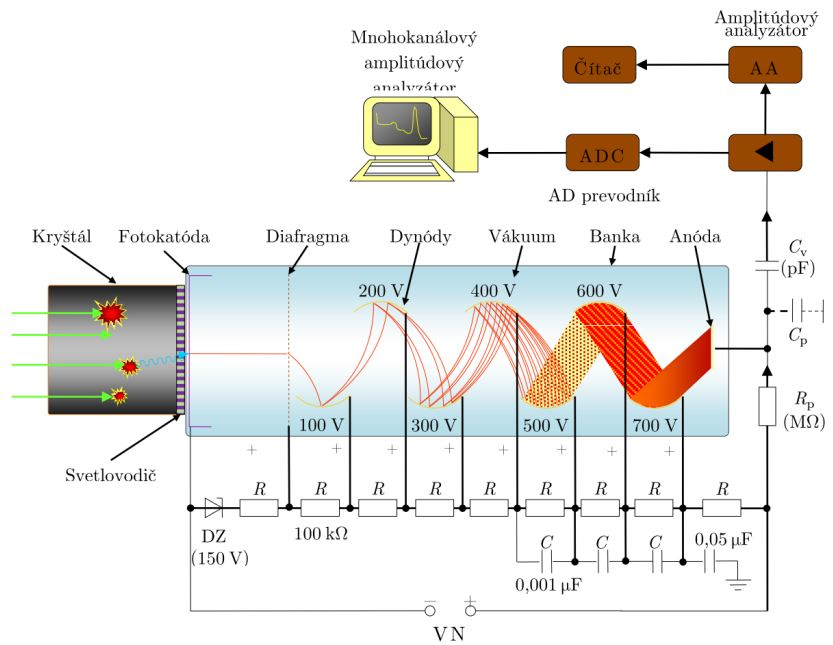
\includegraphics[width=0.65\textwidth]{img/scintilak.JPG}
    \caption{Princip scintilačního detektoru.}
\end{figure}

Scintilační krystal může být:

\begin{itemize}
    \item \textbf{Anorganický} -- primárně pro spektrometrii (gamma). 
    \item[-] Krystal je tvořen nejčastěji alkalickými kovy s malou příměsí nečistoty (tzv. aktivátor, to co je v závorce a ten je zodpovědný za luminiscenci): NaI(Tl), CsI(Tl), CaI(Na), LiI(Eu), CaF$_2$(Eu). 
    \item[-] Pro nízkoenergetické je lepší krystal s malým $Z$, pro vysokoenergetické s velkým $Z$ (ale tam je potom menší energetická rozlišitelnost).  
    \item \textbf{Organický} -- primárně pro neutrony a nabité částice.
    \item[-] Krystal je tvořen organickými molekulami na bázi benzenu a luminiscence je způsobena molekulárními deexcitacemi.
    \item[] Mohou být krystaly (antracen), kapaliny (rozpouštědlo + org. aktivátor, např. toluen + p-terphenyl), plasty (org. aktivátor v polymeru)
\end{itemize}

\textbf{Polovodičové detektory:}

\begin{itemize}
    \item[1)] Ve formě diody z čistého polovodiče v závěrném směru. Gamma záření způsobuje vyrážení elektronů, které se dostávají do vodivého pásma.
    \item[2)] Vznikají tak páry elektron-díra, které jsou nosičemi náboje, čímž vzniká elektrický signál.
    \item[3)] Ten putuje do předzesilovače, zesilovače, tvaruje se a zaznamenává v MCA.
\end{itemize}

Mají mnohem lepší energetickou rozlišitelnost, ale jsou dražší a musejí se chladit (jinak elektrony vyskakují samy a vzniká tak šum). Momentálně nejlepším detektorem je superčistý krystal germania (HPGe).

\textbf{Rozdíly:} polovodičové detektory mají lepší energetickou rozlišitelnost, ale menší detekční účinnost. Také jsou levnější.

\subsubsection{Základní charakteristiky}

\textbf{Odeva detektoru:} poměr mezi energií záření a pozorovaným výstupem (binem) na detektoru (záření o energii $E$ vytvoří $N$ nosičů náboje, které způsobí napěťový rozdíl na elektrodách detektoru, což je to, co detektor zaznamená).

\textbf{Odezvová funkce:} vyjadřuje pravděpodobnost, že monoenergetické fotony budou zaznamenané v daném energetickém binu.

\textbf{Časová odezva detektoru:} čas potřebný k vytvoření signálu. Signál je ve tvaru ostré náběžné a pozvolné seběžné hrany.

\textbf{Časové rozlišení:} nejmenší časová rozlišitelnost mezi dvěmi signály.

\textbf{Citlivost detektoru:} schopnost detektoru produkovat měřitelný signál pro konkrétní typ částice s danou energií. závisí na účinných průřezech, rozměrech hmotnosti, materiálech, šumu (ten může růst s rostoucím rozměrem detektoru).

\textbf{Mrtvá doba:} čas potřebný na zpracování signálu.

\textbf{Energetické rozlišení} nejmenší energetická rozlišitelnost mezi dvěmi signály. Detektor s dobrým rozlišením má užší a vyšší peak, než detektor s horším rozlišením (ale plochy pod peakem jsou stejné).

\textbf{FWHM} = Full Width at Half Maximum, stanovuje šířku pulzu (peaku) v polovině jeho maxima. Dáno energetickým rozlišením. Z toho je možné stanovit relativní energetické rozlišení jako:

$$ R = \dfrac{\text{FWHM}}{E}. $$

Polovodičové detektory mají $R \approx 1$ \%, scintiláky $R \approx 3-10$ \%.

\textbf{Detekční účinnost:} poměr mezi počtem registrovaných částic a emitovaných částic.

\subsubsection{Kalibrace detektorů}

\textbf{Kalibrace energetického rozlišení:} za pomoci FWHM. Peak si proložím Gaussiánem, určím FWHM a relativní rozlišení. Problém nastává, pokud se peaky překrývají (tzv. \textbf{multiplety}).

\textbf{Energetická kalibrace:} MCA mi dá histogram, který musím zkalibrovat (až 16 tisíc kanálů). Jednotlivým binům za pomoci kalibračních zářičů přiřadím konkrétní energii, přičemž předpokládám lineární závislost (pokud mám více zářičů, je možné uvažovat kvadratickou závislost).

\textbf{Kalibrace na mrtvou dobu:} Pokud máme příliš vysokou mrtvou dobu, dochází ke ztrátám počítání signálů a ke ztrátě informací (větší aktivita může vést k přehlcení detektoru a k nárůstu mrtvé doby). Rozlišujeme:

\begin{itemize}
    \item Nekumulativní mrtvá doba -- události, které nastaly v průběhu mrtvé doby, nejsou zaznamenány, ale nevedou na prodloužení celkové mrtvé doby.
    \item Kumulativní mrtvá doba -- události, které nastaly v průběhu mrtvé doby, nejsou zaznamenány, ale vedou na prodloužení celkové mrtvé doby
\end{itemize}

\begin{figure}[H]
    \centering
    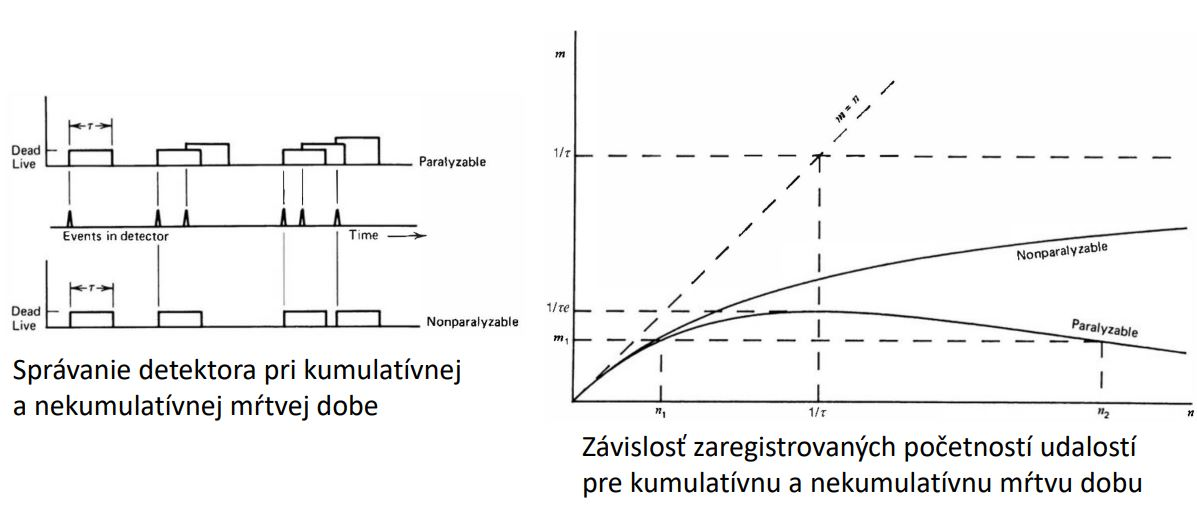
\includegraphics[width=0.8\textwidth]{img/mrtva_doba.JPG}
    \caption{Analýza mrtvé doby.}
\end{figure}

\textbf{Kalibrace detekční účinnosti:} ta není konstantní, je závislá na energii a typu záření. Je zapotřeba stanovit funkci detekční účinnosti za pomoci etalonů o známé aktivitě.

\begin{figure}[H]
    \centering
    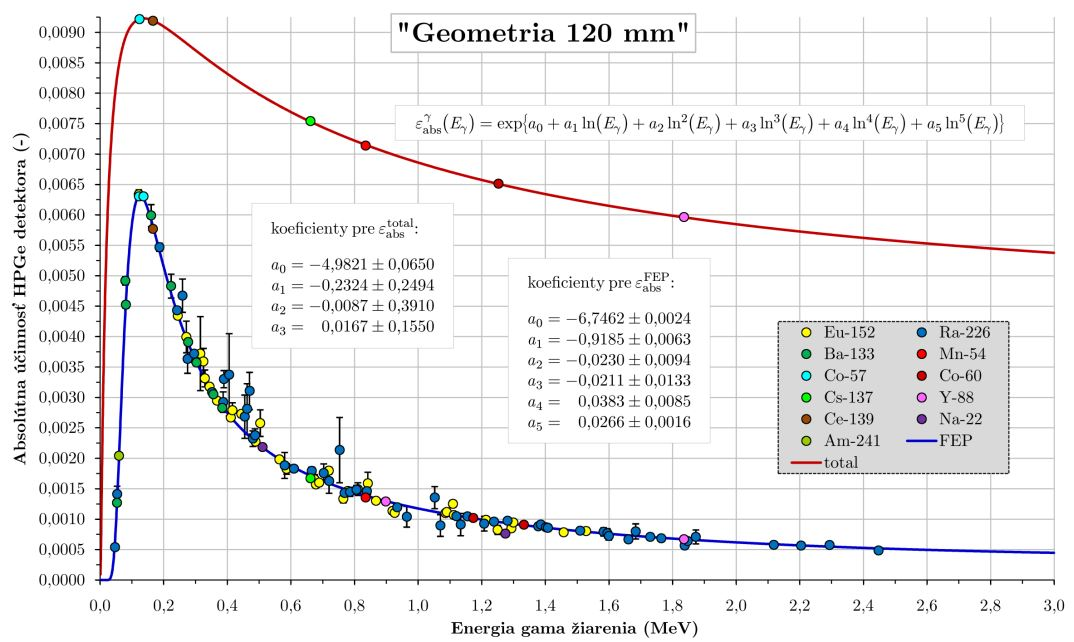
\includegraphics[width=0.8\textwidth]{img/detekcni_krivka.JPG}
\end{figure}

\textbf{Aplikace opravných faktorů:} na závěr je vhodné uvažovat opravné faktory:

\begin{itemize}
    \item oprava na RA rozpad (zářič se v průběhu měření rozpadá),
    \item oprava na nebodovost zdroje,
    \item oprava na samostínění (pro vzorky konečné tloušťky),
    \item oprava na náhodné koincidence (potlačení sumačních efektů).
\end{itemize}

Pak je možné určit finální aktivitu vzorku z analýzi FEP (v pořadí korekce na samostínění, korekce na rozpad a celková aktivita peaku):

$$ \boxed{ A = \dfrac{\mu L}{1 - e^{-\mu L}} \dfrac{\lambda t_\text{real}}{1 - e^{- \lambda t_\text{real}}} \dfrac{S}{I_\gamma \: \varepsilon_\text{FEP}^\text{abs} \: {t_\text{live}}}.} $$


\section[Aktivační měření, gama spektroskopie]{Neutronová pole pro aktivační analýzu, fyzikální principy aktivačních měření, využití gama spektroskopie}

\subsection{Zdroje neutronů}

\subsubsection{Radionuklidové zdroje}

\textbf{Spontánní štěpení:} u některých transuranů existuje nenulová pravděpodobnost, že mimo tradiční rozpady podléhají spontánnímu štěpení. Typickým příkladem je $^{252}$Cf s $T_{1/2} = 2,6$ let a s $\nu = 3,75$ (3,1 \% štěpení, zbytek $\alpha$). Výsledkem je spojité spektrum v oblasti rychlých neutronů (střední energie 2,1 MeV) dle Wattovy distribuce:

$$ \chi(E) = A e^{B E_n} \: \text{sinh} (C \cdot E_n). $$

Emisivita komerčních zdrojů se pohybuje řádově 10$^9$ až 10$^{10}$ 1/s, prodává se ve formě zapouzdřeného oxidu CfO$_2$.

\textbf{($\alpha$,n) reakce:} jde o prahovou reakci na vybraných izotopech, primárně $^9$Be. V tomto důsledku vzniká i doprovodné gamma záření (4,4 MeV pro $^9$Be).

K tomu se přidá $\alpha$ zářič, který emituje primární $\alpha$ částice, a ty vyrážejí sekundární neutrony. Primární zářič se vybírá v závislosti na poločasu rozpadu (ten určuje emisivitu) a doprovodného gamma záření. Jde primárně o $^{210}$Po (poločas 138 dní), $^{238}$Pu (poločas 70 let, skoro žádná gamma), $^{241}$Am (poločas 400 let).

Výsledkem je opět spojité záření (kvůli proměnné energii primární $\alpha$ částice) v rychlé oblasti neutronů. Ve fromě oxidů PoBe, AmBe, PuBe apod. Komerční emisivita 10$^5$ až 10$^9$ 1/s.

\begin{figure}[H]
    \centering
    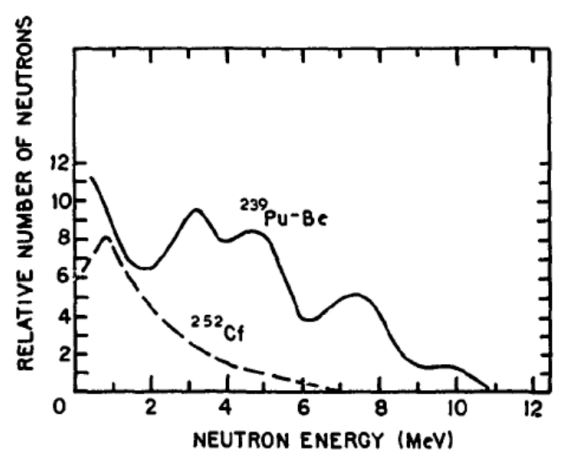
\includegraphics[width=0.4\textwidth]{img/zdroje_E.JPG}
    \caption{Srovnání emitovaného neutronového spektra pro spontánní štěpení a ($\alpha$,n) reakce.}
\end{figure}

\textbf{($\gamma$,n) reakce:} obdobné, opět prahové reakce na vybraných izotopech, primárně $^9$Be (1,67 MeV), $^2$H (2,23 MeV).

Vyžaduje vysokoenergetický gamma zářič ($^{24}$Na, $^{28}$Al, $^{38}$Cl, $^{56}$Mn, $^{226}$Ra). Opět intenzita ovlivněna poločasem rozpadu primárního zářiče.

Výhodou je, že pokud máme monoenergetický primární zářič (není více linek), tak vznikají monoenergetické neutrony. Nevýhoda je, že mají nižší výtěžek a pro vyšší emisivitu (řádově 10$^5$ 1/s) je zapotřebí velmi silné gamma zářiče.

\subsubsection{Zbylé zdroje}

\textbf{Jaderné reaktory:} nejintenzivnější zdroje neutronů, spektrum v závislosti na typu reaktoru, moderace apod. Je možné vytvářet kolimované svazky (radiální kanál + kolimátor (trubka)) o intenzitách 10$^{10}$ 1/s. V pulzním režimu až o několik řádů více.

V případě moderovaných systémů se distribuce může popsat Wattovou formulí, 1/$E^x$ oblastí a Maxwellovým rozdělením.

Dále je možné aplikovat filtry a vytvářet kvazimonoenergetická spektra (Sc, Si, Fe, S apod.).

\textbf{Neutronové generátory:} založeny na prahových reakcích urychlených nabitých částic (D+D, D+T, T+T reakce). Vznikají spojitá spektra s rychlými neutrony o emisivitě až $10^{10}$ 1/s.

Mohou být kompaktní, jdou vypnout, fungují i v pulzním režimu.

\begin{figure}[H]
    \centering
    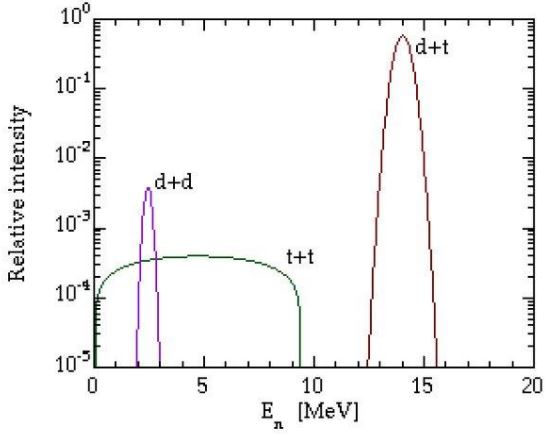
\includegraphics[width=0.4\textwidth]{img/generatory_E.JPG}
    \caption{Emitované spektrum pro neutronové generátory.}
\end{figure}

\textbf{Urychlovačem řízené zdroje:} stejný princip, pouze větší urychlovače, více typů reakcí (jenom změním terčík na $^7$Li, $^9$Be aj.) a mnohem větší emisivita.

Pro tenký terčík získáme čárové spektrum, pro tlustý terčík (před interakcí dojde ke zpomalení primárních částic) spojité spektrum. Využívá se pro výzkumné účely, hlavně pro aktivační měření.

\textbf{Spalačné zdroje:} pokud ještě více zvětším energii primárních částic (řádově GeVy), dojde k rozbití atomu na jednotlivé nukleony, což má za následek mnohem větší emisivitu. Jako terčík se využívají těžké prvky (W, U, Pb apod.). Vzniká široké spojité spektrum (vysokoenergetické, mohou vzniknout neutrony s energií desítek a stovek MeV).

\subsubsection{Zdroje pro aktivační měření}

Nejlepšími neutronovými zdroji pro aktivační měření jsou:

\begin{itemize}
    \item Výzkumné jaderné reaktory:
    \item[-] toky alepoň 10$^9$ 1/cm$^2$/s,
    \item[-] tepelné i epitermální neutrony, primárně (n,$\gamma$) reakce, kde jsou velké účinné průřezy, které jsou dobře proměřené,
    \item[-] případně možnost využít i prahové reakce (n,p), (n,2n) apod.
    \item Urychlovačem řízené zdroje:
    \item[-] toky alepoň 10$^10$ 1/cm$^2$/s,
    \item[-] využívají se reakce p + Be, d + Be
    \item[-] primárně rychlé neutrony ve spojitém spektru (tlustý terčík)
    \item[-] problém je, že v důsledku vícero prahových reakcí se otevírají nové kanály pro vznik daného izotopu. 
    \item Radionuklidové zdroje:
    \item[-] jsou přenositelné
    \item[-] mají menší emisivitu, proto se používají pouze u některých izotopů s vyšším účinným průřezem,
    \item[-] pro NAA jsou vhodné pouze za specifických podmínek. 
\end{itemize}

\subsection{Fyzikální principy aktivačních měření}

Veškeré aktivační měření jsou založeny na tom, že sleduju, které procesy se s daným vzorkem během ozařování v neutronovém procesu odehrály. Díky tomu je možné stanovit parametry neutronového pole, složení (kvantita i kvalita) aj.

\subsubsection{Reakční rychlost}

Vložím-li vzorek do neutronového pole, tak vzniká radioizotop $A$, který se rozpadá do izotopu $B$. Pokud ponecháme izotop v poli alespoň po dobu $10 \cdot T_A$, tak aktivita vzorku bude konvergovat k saturované aktivitě (produkce a destrukce izotopu $A$ je v rovnováze). 

\begin{figure}[H]
    \centering
    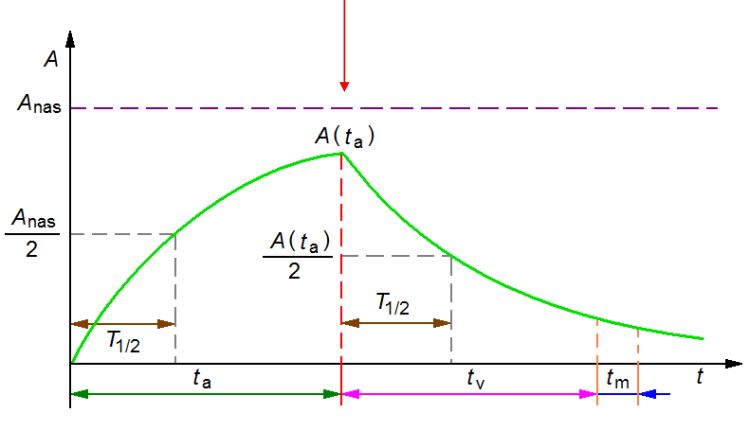
\includegraphics[width=0.6\textwidth]{img/saturovana_aktivita.JPG}
\end{figure}

Po jeho vyjmutí se začne rozpadat, přenese se do laboratoře a začíná se měřit jeho aktivita, ze které je možné zpětně dopočítat \textbf{reakční rychlost} $R$ (1/s), která stanovuje, ke kolika reakcím za jednotku času v daném neutronovém poli docházelo:

$$ \boxed{R = \int_{E_{min}}^{E_{max}} \phi(E) \sigma(E) \: \text{d}E = \dfrac{S \lambda \dfrac{t_\text{real}}{t_\text{live}}}{N_0 \: \varepsilon \: I \: (1-e^{-\lambda t_a}) \: e^{-\lambda t_v} \: (1-e^{-\lambda t_\text{real}}).}} $$

\begin{figure}[H]
    \centering
    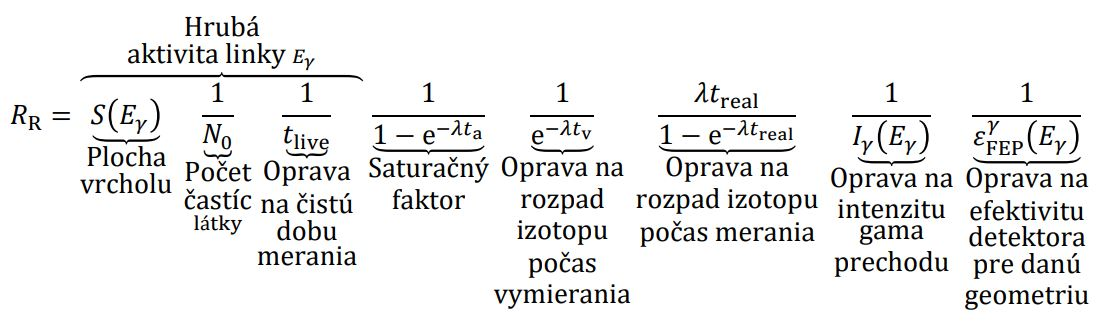
\includegraphics[width=0.8\textwidth]{img/RR_vyznam.JPG}
\end{figure}

Dále je třeba zahrnout vhodné opravné faktory (samostínění, nerovnoměrnost ozařování, geometrie, koincidenční sumační efekty apod.).

Pokud reakční rychlost pronásobím počtem atomů, získám \textbf{produkční rychlost} $R$ (1/s), tedy kolik se vyprodukuje nových izotopů za jednotku času:

$$ \boxed{ P = R \cdot N_0 = \dfrac{S \lambda \dfrac{t_\text{real}}{t_\text{live}}}{\varepsilon \: I \: (1-e^{-\lambda t_a}) \: e^{-\lambda t_v} \: (1-e^{-\lambda t_\text{real}})}.} $$

Pokud produkční rychlost pronásobím korekcí na vymírání, získám \textbf{aktivitu} $A$ (Bq) nově vzniklého izotopu:

$$ \boxed{ A = P \cdot e^{-\lambda t_v} = \dfrac{S \lambda \dfrac{t_\text{real}}{t_\text{live}}}{\varepsilon \: I \: (1-e^{-\lambda t_a}) \: (1-e^{-\lambda t_\text{real}})}.} $$

Navíc pokud skutečně vycházím ze saturované (nebo alespoň skorosaturované) aktivity, je možné vynechat i saturační faktor (je roven jedné), čímž získám stejnou rovnici z předešlé otázky:

$$ A = \dfrac{S \lambda \dfrac{t_\text{real}}{t_\text{live}}}{\varepsilon \: I \: (1-e^{-\lambda t_\text{real}}).} $$

\subsubsection{Generátorové rovnice}

Dále může docházet ke kaskádám, vznikne izotop $A$, který se rozpadá do $B$ a ten do $C$. Po chvíli dochází k rovnováhám mezi izotopy:

\begin{itemize}
    \item \textbf{Přechodná rovnováha} -- pokud $T_A > T_B$, k takovéto rovnováze dojde po uplynutí $10 \cdot T_B$, aktivity jsou v poměru:
    $$ \dfrac{A_B}{A_A} = \dfrac{T_A}{T_A - T_B}. $$
    \item \textbf{Dlouhodobá rovnováha} -- pokud $T_A >> T_B$, jde o limitní případ předešlého, kdy je $T_B$ zanedbatelně malý (okamžitý) a aktivity jsou v rovnováze:
    $$ A_A = A_B $$
    \item \textbf{Stav bez rovnováhy} -- pokud $T_A < T_B $, k rovnováze nedojde.
\end{itemize}

\subsubsection{Aplikace filtrů}

V neutronovém poli moderovaných jaderných reaktorů jsou neutrony o všech energiích, což je z hlediska aktivačního měření problematické (otevírají se nové reakční kanály, např. izotop $^{24}$Na může vzniknout za pomoci $^{23}$Na(n,$\gamma$)$^{24}$Na reakce v jakémkoliv spektru, nebo za pomoci $^{27}$Al(n,$\alpha$)$^{24}$Na v rychlém spektru). 

To je možné eliminovat za pomoci filtrů (kadmium), kdy odstraním efekt neutronů nad kadmiovou hranou. v závislosti na tom rozlišujeme:

\begin{itemize}
    \item ENNA = epitermální NNA,
    \item RNNA = reaktorová NAA.
\end{itemize}

Je možné využít i jiné filtry (B, Cl, Au, In, Al), ale musí být dostatečně tlusté, aby vykompenzovaly to, že nejsou tak dobrými absorbátory. Takto je možné odseparovat jednotlivé oblasti neutronového spektra.

\textbf{$^{113}$Cd} je vhodné pro energie pod 2 eV, nezahřívá se, stačí ho 1 mm, aktivované kadmium rychle vymírá. \textbf{$^{10}$B} je ideální nad 15 eV, nemá žádnou hranu, produkuje alfu, což vede k ohřevu vzorku. \textbf{Cd + B} je vhodné pro energie od 2 do 15 eV. 

\subsection{Využití gamma spektroskopie}

\textbf{Aplikace gamma spektrometrie:}

\begin{itemize}
    \item Zobrazovací metody PIGE a PIXE (viz první okruh otázek)
    \item RTG difrakční krystalografie
    \item Neutronová aktivační analýza
\end{itemize}

\textbf{Základní výzkum:}

\begin{itemize}
    \item Studium rozpadových schémat (Stanovení intenzit, poločasů rozpadů, gamma linek apod.)
    \item Studium účinných průřezů
    \item Aktivační měření neutronových polí
\end{itemize}
\section[Aktivační analýza]{Druhy a metody neutronové aktivační analýzy, pracovní procedury a praktické aplikace neutronové aktivační analýzy}

\textbf{Neutronová aktivační analýza} je radioanalytická metoda založená na jaderné aktivaci chemických prvků přítomných v analyzovaným vzorku. Patří mezi nejcitlivější chemické analýzi.

Existují i další aktivační analýzy založené na primárních fotonech, jiných nabitých částicích či vysokoenergetických neutronech, nicméně ty jsou komplikovanější (ale zase mohou objevit jiné prvky). NAA je totiž citlivá na velikosti účinných průřezů na daných prvcích (pokud je účinný průřez dostatečný, je možné zaznamenat i nepatrné stopové množství). Nejčastěji se tedy využívá neutronová analýza s tepelnými neutrony, kde jsou velmi vysoké účinné průřezy (n,$\gamma$) reakcí.

\begin{figure}[H]
    \centering
    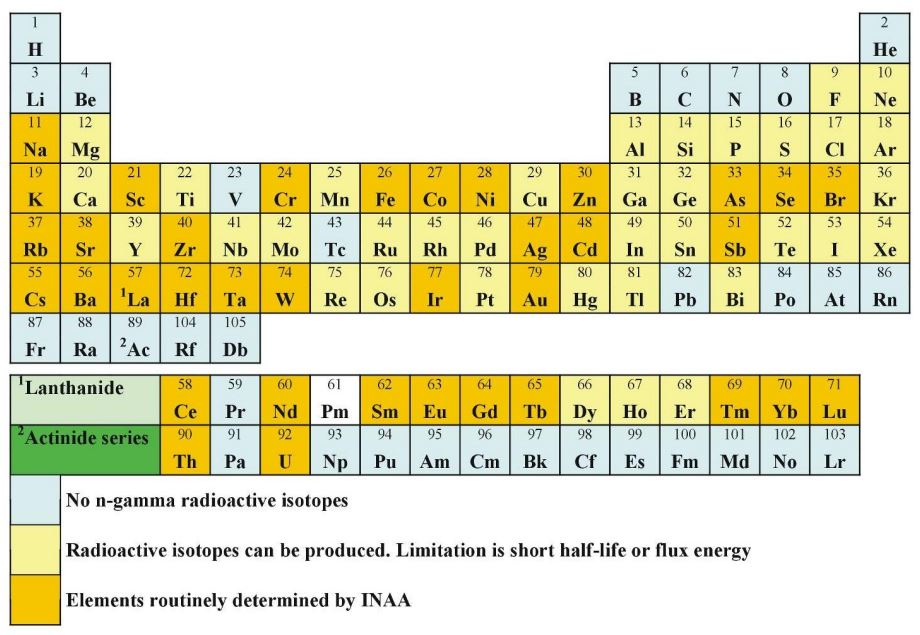
\includegraphics[width=0.65\textwidth]{img/prvky_NAA.JPG}
    \caption{Prvky vhodné pro NAA.}
\end{figure}

\subsection{Základní dělení}

Rozlišujeme:

\begin{itemize}
    \item \textbf{Kvalitativní NAA} -- zajímá mě pouze, které prvky se ve vzorku nacházejí.
    \item \textbf{Kvantitativní NAA} -- zajímá mě, v jakém množství se prvky ve vzoru nacházejí.
\end{itemize}

Dále dle energie neutronů (lze ovlivnit filtry): tepelné, epitermální, rychlé.

\subsubsection{Absolutní NAA}

Pokud známe přesnou hustotu neutronového toku a průběh účinného průřezu, tak je možné ze znalosti reakční rychlosti přesně dopočíst hmotnost zkoumaného izotopu. Hustotu toku ale přesně většinou neznám, proto se moc nevyužívá. Ale je vhodná, pokud dopředu nevím co hledám.

\begin{equation}
    \boxed{
        m = \dfrac{S \lambda \dfrac{t_\text{real}}{t_\text{live}}}{I_\gamma \: \varepsilon_\text{FEP}^\text{abs} \: \left( 1 - e^{-\lambda t_a} \right) e^{-\lambda t_v} \left( 1 - e^{-\lambda t_\text{real}} \right) \dfrac{N_A}{M} \int \sigma(E) \phi(E) \: \text{d}E}.
    }
\end{equation}

\subsubsection{Porovnávací NAA}

Pokud dopředu vím, co hledám, tak spolu se vzorkem ozářím etalon z daného materiálu o známé hmotnosti. Za předpokladu rovnosti produkčních rychlostí ve vzorku i v etalonu pak přes trojčlenku dopočtu množství izotopu ve vzorku. Vyhnu se neznalosti neutronového toku a účinných průřezů, ale pro každý izotop musím mít vlastní standard a oboje ozařovat za stejných podmínek.

\begin{equation}
    \boxed{
        m = m_\text{et} \dfrac{P}{P_\text{et}}.
    }
\end{equation}

\subsubsection{Metoda jednoho komparátoru}

Něco mezi přímou a porovnávací metodou. Využívá tzv. k-faktory pro jednotlié prvky, tedy poměr ozářených aktivit mezi standartem a daným prvkem. Tyto faktory se pak určují buď výpočtem (složité), nebo experimentálně (společným ozářením). Experimentálně získané k-faktory jsou pak přesnější, ale je možné je využít pouze pro daný detektor, reaktor a geometrii a za předpokladu stabilního neutronového pole. Jsou nepřenositelné.

Pak stačí spolu se vzorkem ozářit pouze etalon se standardem a za pomoci dopředu známých k-faktorů určit i-tý prvek.

\begin{equation}
    \boxed{
        m = k_i m_\text{com} \dfrac{P}{P_\text{com}}.
    }
\end{equation}

\subsubsection{Metoda $k_0$ standardizace}

Zdokonalení předchozí metody, k porovnávání jsou využity $k_0$ faktory, které jsou přenositelné. Spolu se vzorkem se ozáří komparátor (zlato), ke kterému jsou tabelovány hodnoty $k_0$ a $Q_0$.

\begin{equation}
    \boxed{
        m = m_\text{com} \dfrac{P \: I}{P_\text{com} \: I_\text{com}} \dfrac{1}{k_0} \dfrac{1 + \dfrac{Q_0^\text{com}}{f}}{1 + \dfrac{Q_0}{f}}, \: \: \: f = \dfrac{\phi_\text{th}}{\phi_\text{epi}}.
    }
\end{equation}

Hodnoty $\phi_\text{th}$ a $\phi_\text{epi}$ se pak stanoví aktivačním měřením neutronového pole za pomoci změření reakčních rychlostí v tepelné a epitermální oblasti na zlatém komparoátoru/standardu s a bez kadmiového filtru na základě \textbf{Hoghdalovy konvence}.

Platí, že spektrum v reaktoru je možné rozepsat do 3 složek (štěpné Wattovo, 1/v Fermiho a tepelné Maxwellovo), které je možné mezi sebou provázat pomocí empirických spojovacích funkcí. Konvence pak říká jak je možné stanovit reakční rychlosti v těchto grupách na základě měření s a bez kadmiového filtru (ještě třeba pronásobit kadmiovým faktorem, ten najdu na internetu nebo si ho pamatuju $f_\text{Cd}=1.16$ (VR-1)):

$$ R_\text{th} = R - f_\text{Cd}R_\text{Cd}, $$
$$ R_\text{epi} = f_\text{Cd}R_\text{Cd}. $$

Potom platí:

$$ \phi_\text{th} = \dfrac{P_\text{th}}{g(T_0) \: \sigma_0 \: G_\text{th}}, $$
$$ \phi_\text{epi} = \dfrac{P_\text{epi}}{I_0 \: G_\text{epi}}, $$

kde $g(T_0)$ je opravný faktor pro oblast 1/v, $G$ je korekční faktor pro samostnínění, $\sigma_0$ průřez pro (n,$\gamma$) reakci na etalonu při energii $E_0$ a $I_0$ je rezonanční integrál pro energii $E_0$:

\begin{equation}
    \boxed{
        m = m_\text{Au} \dfrac{P I}{P_\text{Au} I_\text{Au}} \dfrac{1}{k_0} \dfrac{G_\text{th,Au} f + G_\text{epi,Au} Q_{0\text{,Au}}}{G_\text{th} f + G_\text{epi} Q_{0}}, \: \: \: Q_0 = \dfrac{I_0}{\sigma_0}.
    }
\end{equation}

Dále ještě existuje metoda stanovení $k_0$ standardizace za pomoci \textbf{Westcottova formalizmu}, ale to jsme nedělali :).

\subsection{Pracovní postup}

\begin{itemize}
    \item[1)] Vzorek připravím k ozáření (pevné vzorky přilepím izolepou, případně nějaká chemická separace biologických vzorků) a vložím do neutronového pole. Případně přidám etalon.
    \item[2)] Ozařuji vzorek po dobu $t_a$.
    \item[3)] Přenesu vzorek do laborky a připravím k měření (doba $t_v$).
    \item[4)] Změřím gamma spektrum (doba $t_\text{real}$) a určím produkční rychlosti jednotlivých FEP peaků.
    \item[5)] Dle konkrétní metody přepočtu produkční rychlost na hmotnost. Pokud má izotop vícero linek, tak provedu analýzu pro všechny peaky, ze kterých určím vážený průměr.
\end{itemize}

Měření je možné optimalizovat:

\begin{itemize}
    \item opakováním měření, 
    \item použití vícero peaků,
    \item delší doba měření $t_\text{real}$,
    \item kratší doba vymírání $t_v$,
    \item delší doba aktivace $t_a$ (ideálně do saturovaného stavu),
    \item co nejmenší mrtvá doba,
    \item cyklicky ozařovat (nutné pro krátkodobě žijící izotopy, např. $^{20}$F. Pak je možné změřit i izotopy s poločasy rozpadu v jednotkách vteřin).
\end{itemize}


\subsection{Využití NAA}

NAA se uplatňuje v:

\begin{itemize}
    \item archeologie (kosti mamutů, nádobí),
    \item geologie (složení hornin, vyvřelin),
    \item historie,
    \item biomedicína,
    \item výživové produkty (složení doplňků stravy),
    \item průmysl,
    \item apod.
\end{itemize}

Jde o částečně destruktivní metodu (problém jsou živé organismy, které pravděpodobně umřou).
\section[Měření neutronů aktivační metodou]{Stanovení neutronových polí, účinných průřezů a štěpných výtěžků využitím aktivační techniky}

Většina důležitých informací je v otázkách 9-11.

\subsection{Aktivační měření s dozimetrickými foliemi}

Měření probíhá tak, že vložíme aktivační detektor (folie o známé tloušťce, hmotnosti a materiálu) do neutronového pole a poté za pomoci spektrometrie určíme reakční rychlost:

\begin{equation}
    \boxed{R = \int_{E_{min}}^{E_{max}} \phi(E) \sigma(E) \: \text{d}E = \dfrac{S \lambda \dfrac{t_\text{real}}{t_\text{live}}}{N_0 \: \varepsilon \: I \: (1-e^{-\lambda t_a}) \: e^{-\lambda t_v} \: (1-e^{-\lambda t_\text{real}}),}}
\end{equation}

případně produkční rychlost (furt ty samé vztahy):

\begin{equation}
    \boxed{P =  \dfrac{S \lambda \dfrac{t_\text{real}}{t_\text{live}}}{\varepsilon \: I \: (1-e^{-\lambda t_a}) \: e^{-\lambda t_v} \: (1-e^{-\lambda t_\text{real}}).}}
\end{equation}

Tato měření pak pomohou pomoct v dalších odvětvích (teď mimo NAA, té se věnuje předešlá otázka).

\subsubsection{Měření účinných průřezů}

Hojně využívané pro měření účinných průřezů prahových reakcí (na urychlovači). Jako zdroj neutonů se použije svazek protonů, které odstřelují tenkou Li folii (p + Li), což produkuje proud kvazimonoenergetických neutronů, které jsou dobře odlišitelné od pozadí. Dále možné využít beryliový terčík (p + Be).

\begin{figure}[H]
    \centering
    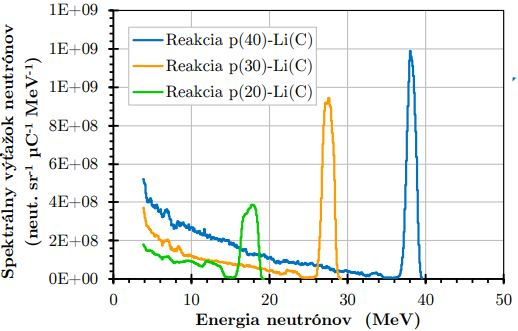
\includegraphics[width=0.5\textwidth]{img/p+Li_E.JPG}
    \caption{Neutronové spektrum pro reakci (p + Li).}
\end{figure}

Tím, jak měním rychlost primárních protonů jsem schopný sekundární neutronový peak posouvat do různých energiích. Tyto sekundární neutrony poté ozařují zkoumaný materiál, jehož účinný průřez měřím. Takto změřím někoik bodů (dle energie), které poté vyhodnocuji a dle čehož stanovím závislost $\sigma$ na $E$. Tato metoda se využívá v ÚJF AV ČR v Řeži.

\subsubsection{Spektrometrie neutronových polí}

Spektrometrii neutronů je věnována celá předchozí otázka, tahle kapitolka je pouze o smektrometrii aktivační technikou. Ve zkoumaném neutronovém poli se ozáří několik odlišných aktivačních detektorů: Cd, Mo, Y, Cu, In, Co apod., přičemž materiály se vybírají podle toho, jak jsou citlivé v jiných oblastech energie neutronů.

Po ozáření opět proběhne gamma spektrometrie a u každé folie se stanoví sada reakčních rychlostí. Jelikož známe průběhy účinných průřezů na těchto materiálech, je pak možné zpětně zrekonstruovat neutronové spektrum. K tomu se využívají různé kódy, my pracovali s kódem SAND-II (podobně jako v případě měření Bonnerovými sférami).

\begin{figure}[H]
    \centering
    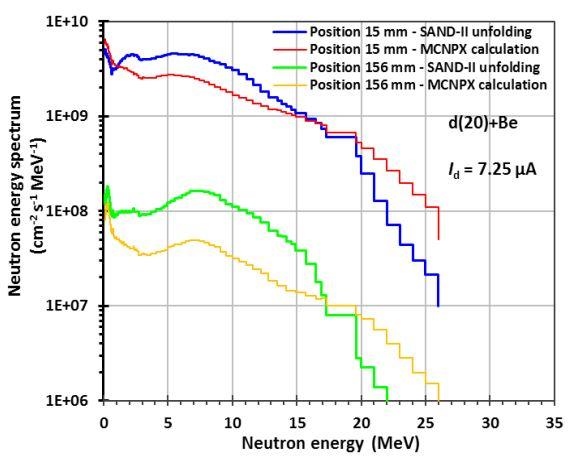
\includegraphics[width=0.5\textwidth]{img/spektrum_aktivacne.JPG}
    \caption{Zpětná rekompozice neutronového spektra pro reakci (d + Be).}
\end{figure}

\subsubsection{Stanovení štěpných výtěžků}


Aktivační metoda (neutron activation analysis, NAA) představuje klíčový nástroj pro kvantitativní analýzu štěpných produktů vznikajících při štěpení těžkých jader, jako je $^{235}$U nebo $^{239}$Pu. Tato metoda využívá měření gama záření emitovaného radionuklidy po jejich aktivaci neutrony a umožňuje stanovit relativní štěpné výtěžky jednotlivých produktů s vysokou přesností. Tato práce se zaměřuje na detailní popis principů NAA, její aplikaci na výpočet štěpných výtěžků a diskusi výhod a omezení této metody.

Štěpné výtěžky představují základní charakteristiku jaderného štěpení, vyjadřující relativní množství jednotlivých produktů vznikajících při této reakci. Přesné stanovení těchto výtěžků je nezbytné pro mnoho aplikací, včetně návrhu jaderných reaktorů, správy jaderného odpadu a základního výzkumu jaderné fyziky. Aktivační metoda (NAA) nabízí možnost měření s vysokou citlivostí a selektivitou, což ji činí oblíbenou pro analýzu produktů štěpení.

\subsubsection*{Princip metody}

NAA je analytická technika založená na ozařování vzorku neutrony a následném měření gama záření emitovaného radionuklidy. Celý proces lze rozdělit do následujících kroků:

\begin{enumerate}
    \item Vzorek obsahující štěpný materiál (např. $^{235}$U nebo $^{239}$Pu) je umístěn do vhodného kontejneru, který odolá neutronovému ozařování. Velikost a geometrie vzorku jsou optimalizovány pro dosažení rovnoměrného ozáření.
    \item Vzorek je ozářen neutrony ve zdroji, například v jaderném reaktoru. Během ozáření probíhá štěpení těžkých jader, přičemž vznikají produkty štěpení, které jsou často samy o sobě radioaktivní. Současně dochází k aktivaci přítomných prvků.
    \item Po ozařování je vzorek přemístěn do gama spektrometru. Radioaktivní produkty emitují gama záření, jehož energie jsou charakteristické pro konkrétní radionuklidy. Intenzita jednotlivých gama čar je přímo úměrná množství daného radionuklidu ve vzorku.
    \item Na základě změřených intenzit gama záření a znalosti detekční účinnosti, poločasů rozpadu a dalších parametrů lze vypočítat počet jader jednotlivých produktů štěpení. Relativní štěpné výtěžky se stanoví podle vztahu:
\begin{equation}
    \boxed{Y_i = \frac{N_i}{\sum_j N_j},}
\end{equation}
kde $N_i$ je počet jader i-tého produktu a $\sum_j N_j$ je celkový počet jader všech detekovaných produktů štěpení.
\end{enumerate}

\textbf{Výhody:}

\begin{itemize}
    \item Vysoká citlivost: Detekce stopových množství radionuklidů.
    \item Selektivita: Identifikace specifických radionuklidů díky charakteristickým energiím gama záření.
    \item Nedestruktivní charakter: Vzorek lze použít pro další analýzu.
\end{itemize}

\textbf{Omezení:}

\begin{itemize}
    \item Vyžaduje přístup k neutronovému zdroji, což omezuje její dostupnost.
    \item Náročné zpracování dat, zejména při překryvu gama čar.
    \item Manipulace s radioaktivními vzorky vyžaduje přísná bezpečnostní opatření.
\end{itemize}

\textbf{Aplikace:}

Metoda NAA je široce využívána v následujících oblastech:

\begin{itemize}
    \item Studium produktů štěpení při různých energiích neutronů.
    \item Výzkum vlastností jaderného paliva.
    \item Analýza radioaktivních odpadů.
\end{itemize}

Stanovení štěpných výtěžků pomocí aktivační metody je účinným nástrojem pro studium jaderných procesů. Tato metoda poskytuje přesná a spolehlivá data o relativních výtěžcích jednotlivých štěpných produktů, což přispívá k hlubšímu pochopení jaderného štěpení a jeho aplikací.

\section[Využití výzkumných reaktorů]{Využití výzkumných reaktorů jako zdrojů neutronů}

Výzkumné jaderné reaktory hrají klíčovou roli v rozvoji jaderné vědy a technologií. Na rozdíl od energetických reaktorů, jejichž primární účel je výroba elektřiny, výzkumné reaktory slouží především k experimentálním, vzdělávacím a vývojovým účelům. Jsou navrženy tak, aby umožnily detailní studium neutronových polí, testování nových konstrukčních materiálů, vývoj jaderného paliva a získávání cenných dat pro validaci výpočetních metod a simulací.

Tyto reaktory také poskytují neutronové zdroje pro aplikace v medicíně (např. produkce radionuklidů pro diagnostiku a terapii), průmyslu (neutronová radiografie) a vědě (materiálový výzkum pomocí neutronového rozptylu). Díky své flexibilitě a schopnosti simulovat různé provozní podmínky hrají nezastupitelnou roli při řešení aktuálních výzev spojených s jadernou bezpečností, udržitelností a inovacemi v oblasti jaderné energetiky.

V České republice se výzkumné reaktory staly významnou součástí jaderného výzkumu. Mezi nejvýznamnější zařízení patří reaktory LVR-15, LR-0 v Řeži a VR-1, VR-2, které poskytují zázemí pro experimentální měření, přípravu odborníků a mezinárodní spolupráci. Výzkumné reaktory tak nejen podporují technický pokrok, ale také přispívají k mezinárodnímu sdílení poznatků a k budoucímu rozvoji celého oboru.

Informace ohledně způsobů využití jednotlivých výzkumných reaktorů na světě lze dohledat v databázi IAEA, Research Reactor Database. Nachází se tam veškeré informace ohledně vše výzkumných reaktorů, ve vše provozních stavech (plánované, ve výstavbě, v provozu, krátkodobě odstavené, dlouhodobě odstavené I vyřazené z provozu). 

Způsoby využití lze rozdělit například podle toho, jestli se využívá přímo AZ reaktoru (uvnitř reaktoru) nebo jestli je reaktor pouze jako zdroj neutron (vně reaktoru). Tak trochu mimo leží vzdělávání a výcvik:

\begin{table}[h!]
\centering
\caption{Výzkumné reaktory v provozu, dočasně odstavené, plánované a ve výstavbě.}
\begin{tabular}{lrr}
\toprule
Stav reaktoru & Počet reaktorů & Počet zemí \\
\midrule
Celkem & 257 & 56 \\
Výuka / školení & 161 & 51 \\
Neutronová aktivační analýza & 116 & 50 \\
Výroba radioizotopů & 82 & 41 \\
Materiální ozařování & 68 & 26 \\
Neutronová radiografie & 69 & 37 \\
Neutronový rozptyl & 44 & 28 \\
Dopování křemíku & 23 & 15 \\
Geochronologie & 24 & 21 \\
Barvení drahokamů & 20 & 12 \\
Zachytávání neutronů borem pro terapii & 15 & 12 \\
Inovativní výzkum energie &  &  \\
Příprava jaderných dat & 16 & 9 \\
Další aplikace & 116 & 34 \\
\bottomrule
\end{tabular}
\end{table}

\subsection{Neutronová aktivační analýza}

Neutronová aktivační analýza (NAA) je jaderná analytická technika využívaná pro stanovení:

\begin{itemize}
    \item Složení vzorků
    \item Nečistot ve vzorcích
    \item Stopových prvků ve vzorcích
\end{itemize}

NAA umožňuje získat jak kvalitativní, tak kvantitativní výsledky. Stabilní nuklidy po interakci s neutrony mohou vytvářet nestabilní izotopy. Tyto nestabilní izotopy jsou následně analyzovány pomocí vícekanálového analyzátoru. 

Z detekované gama záření lze určit původní stabilní nuklidy, které byly ve vzorku přítomny před jeho ozářením. Tato technika je velmi užitečná pro přesné analýzy složení vzorků a sledování příměsí či stopových prvků.

Existuje několik typů neutronové aktivační analýzy, z nichž každá má specifické aplikace a vlastnosti:

\begin{itemize}
    \item \textbf{Instrumentální NAA (INAA)}: Standardní metoda bez chemické separace.
    \item \textbf{Cyklická instrumentální NAA (CINAA)}: Používá opakované cykly ozařování a měření.
    \item \textbf{Epithermální instrumentální NAA (EINAA)}: Využívá epithermální neutrony.
    \item \textbf{Radiochemická NAA (RNAA)}: Zahrnuje chemickou separaci před měřením.
    \item \textbf{Předkoncentrační NAA (PNAA)}: Před analýzou je prováděna předkoncentrace vzorku.
    \item \textbf{Odvozená NAA (DNAA)}: Modifikace zahrnující derivace vzorku.
    \item \textbf{Promptní gama NAA (PGNAA)}: Detekce gama záření během ozařování.
    \item \textbf{Zpožděná gama NAA (DGNAA)}: Detekce gama záření po určitém zpoždění od ozařování.
\end{itemize}

NAA má širokou škálu využití např. v archeologii, geologii, geochemii, biomedicíně, nutriční a zdravotní vědě, a vědách týkající se životního prostředí. Příklady z VR-1: tibetské mince, zdravotní doplňky, mamutí kosti enviromentální vzorky, vzorky lidské tkáně atd.

\subsection{Ozařování materiálů}

Ozařování materiálů se provádí z různých oblastech např. testování nových typů paliv, změny materiálu vlive záření, teploty, tlaku atd. především pro použití v jaderných elektrárnách nebo nových typech reaktorů.

Lze použít speciální ozařovací místa, speciální smyčky s prostředím, tlakové nádoby atd.

\subsection{Měření jaderných dat}

Výzkumné reaktory mohou být také používány k ověřování jaderných dat -- data ze štěpení (výtěžky ze štěpení), data účinných průřezů, data o zpožděných neutronech, rozpadová data atd.

\subsection{Produkce radioizotopů}

Radioizotopy jsou používány v široké škále aplikací -- medicína, průmysl, zemědělství, věda a výzkum. Příklady nejpoužívanějších radioizotopů jsou:
\textsuperscript{14}C, \textsuperscript{24}Na, \textsuperscript{32}P, \textsuperscript{35}S, \textsuperscript{38}Cl, \textsuperscript{41}Ar, \textsuperscript{51}Cr, \textsuperscript{56}Mn, \textsuperscript{60}Co, \textsuperscript{54}Cu, \textsuperscript{89}Sr, \textsuperscript{99m}Tc, \textsuperscript{125}I, \textsuperscript{131}I, \textsuperscript{133}Xe, \textsuperscript{153}Sm, \textsuperscript{169}Yb, \textsuperscript{170}Tm, \textsuperscript{192}Ir, \textsuperscript{198}Au, \textsuperscript{177}Lu.

Pro nemedicínské aplikace jsou nejčastěji produkovány dva radioizotopy: \textsuperscript{60}Co a \textsuperscript{192}Ir (zdroje gama záření). Tyto izotopy jsou používány v oblastech jako gama zobrazování, gama radioterapie, kalibrační zařízení, sterilizace nástrojů apod. 

V medicínské oblasti je nejčastěji používán \textsuperscript{99m}Tc z \textsuperscript{99}Mo. Tento izotop se využívá v 80\,\% případů diagnostiky nádorů pomocí radioizotopů. \textsuperscript{99}Mo vzniká jako produkt ze štěpení \textsuperscript{235}U. Uranový vzorek je ozářen v reaktoru, kde vznikne štěpením \textsuperscript{99}Mo, který je následně přepracován do tekuté formy.

    \[
        {}^{99}_{42}\mathrm{Mo} \xrightarrow{\beta^-} {}^{99m}_{43}\mathrm{Tc} \xrightarrow{\gamma} {}^{99}_{43}\mathrm{Tc}
    \]
    \[
        T_{1/2} = 66.924\,\mathrm{h}, \quad T_{1/2} = 6.0072\,\mathrm{h}
    \]

\begin{figure}[H]
    \centering
    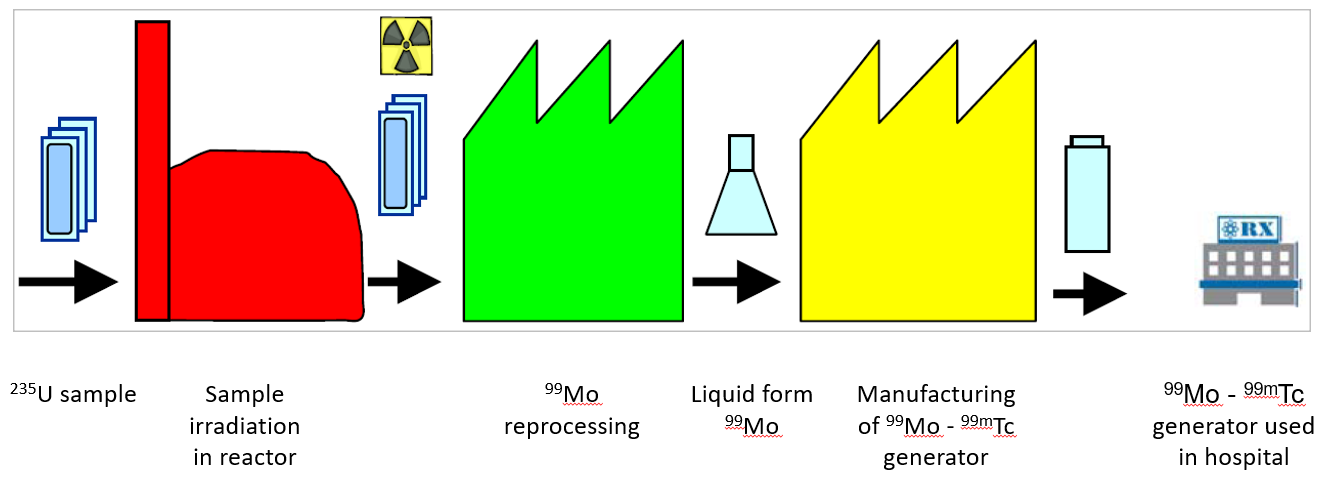
\includegraphics[width=0.7\linewidth]{img/CestaRadioizotopu.png}
    \caption{Cesta radioizotopu}
    \label{fig:enter-label}
\end{figure}

Jsou potřebné vysoké neutronové toky, přibližně $10^{13} - 10^{14}\,\mathrm{n/s/cm^2}$. V současnosti provozované reaktory pro produkci \textsuperscript{99}Mo jsou: BR2 (Belgie), HRF (Nizozemsko), LVR-15 (Česko), OPAL (Austrálie), MARIA (Polsko), RA-3 (Argentina), Itálie (Pavia)

\subsection{Transmutace -- dopování křemíku a barvení kamenů}

\textbf{Dopování křemíku:}

Během ozařování křemíkových ingotů tepelnými neutrony v reaktoru dochází ke vzniku nečistot, což zlepšuje vodivost křemíkového polovodiče. Přírodní křemík obsahuje cca 3 \% $^{30}$Si, který je vhodný k dopování. 

 \[
{}^{30}_{14}\mathrm{Si} + {}^{1}_{0}\mathrm{n} \rightarrow {}^{31}_{14}\mathrm{Si} + \gamma
\quad \text{a} \quad
{}^{31}_{14}\mathrm{Si} \rightarrow {}^{31}_{15}\mathrm{P} + \beta^-
\]

Křemík je čtyřmocný prvek, zatímco fosfor je pětimocný. Když se v matrici krystalů křemíku vytvoří fosfor, čtyři z jeho valenčních elektronů vytvoří vazby podobné okolním atomům křemíku a extra valenční elektron se uvolní. Tento volný elektron v krystalu je dostupný jako volný nosič náboje, který mění vodivost krystalu.

Křemík je k tomuto nejvhodnější, ale existují i jiné materiály např. germanium. Opět jsou potřeba vysoké neutronového toky cca 10$^{13}$ - 10$^{14}$ n/s.cm$^2$. 

\textbf{Barvení drahých kamenů:}

Barvení drahokamů je založeno na myšlence, že po ozáření mohou některé drahokamy změnit svou barvu na atraktivnější a hodnotnější. 

Ozáření může být provedeno rychlými neutrony nebo vysokoenergetickým gama zářením. Nádoby jsou stíněné (bór, kadmium) za účelem potlačení ozáření tepelnými neutrony a použití pouze rychlých neutronů (10$^{13}$ - 10$^{14}$ n/s.cm$^2$). Po ozáření je nutné nechat klesnou aktivitu, doba zaleží na typu kamenů, ale obvykle několik měsíců.

Drahé kameny se obvykle vkládají do ozařovacího kontejneru o hmotnosti asi 2 kg kamenů, které se nakládají k aktivní zóně. Dominantně je ozařován topaz, který po ozáření mění barvu z bílé/průhledné na modrou. V některých zemích je barvení drahokamů zakázáno. V Řeži to dělali, ale už to mají zakázané.

\subsection{Neutronové zobrazování}

Neutronové zobrazování je metoda určená k pozorování vnitřních struktur neprůhledných objektů. Jedná se o nedestruktivní metodu. Funguje na stejném principu jako rentgenové zobrazování. Rozdíl je pouze v interakci neutronu s látkou, což poskytuje jiný kontrast než rentgen. Mezi další zobrazovací metody patří například:

\begin{itemize}
    \item Rentgenové zobrazování
    \item Gama zobrazování
\end{itemize}

\begin{figure}[H]
    \centering
    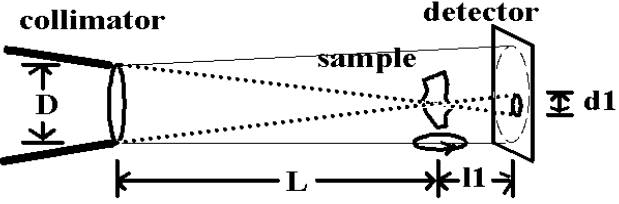
\includegraphics[width=0.7\linewidth]{img/SestavanaNZ.png}
    \caption{Neutronové zobrazování}
    \label{fig:enter-label}
\end{figure}

Základní princip: Intenzita paprsku je po průchodu zobrazovaným objektem utlumena v závislosti na tloušťce a materiálu objektu. Útlum je dán materiálovým složením vzorku -- míra pravděpodobnosti interakce je dána účinným průřezem. Toto zeslabení závisí na:

\begin{itemize}
    \item Tloušťce objektu
    \item Materiálu, ze kterého je objekt vyroben
\end{itemize}

Existuje několik metod NI (neutron imaging): neutronová radiografie (2D zobrazování -- vytváří se pouze 2D obraz zobrazovaného předmětu), neutronová počítačová tomografie (3D zobrazování -- pomocí sady 2D obrazů pod různými úhly lze počítačově provést 3D rekonstrukci obrazu), stroboskopické zobrazování (zobrazování dynamických procesů). Nově patří do neutronového zobrazování i další pokročilé metody: energeticky selektivní zobrazování (používá se velmi úzké neutronové spektrum), neutronová mřížková interferometrie, zobrazování pomocí polarizovaných neutronů, zobrazování ve vysokém rozlišení.

Dříve se používaly jako detektory fotografické filmy s konvertorem neutronů, v současnosti se používají digitální systémy založení na kombinaci kamera (CCD nebo CMOS) scintilátor. 

NI má širokou škálu použití např. archeologie, kulturní dědictví, jaderný průmysl, výzkum palivových článků, výzkum baterií, environmentální věda -- rostliny, průmyslové výrobky atd.

\begin{figure}[H]
    \centering
    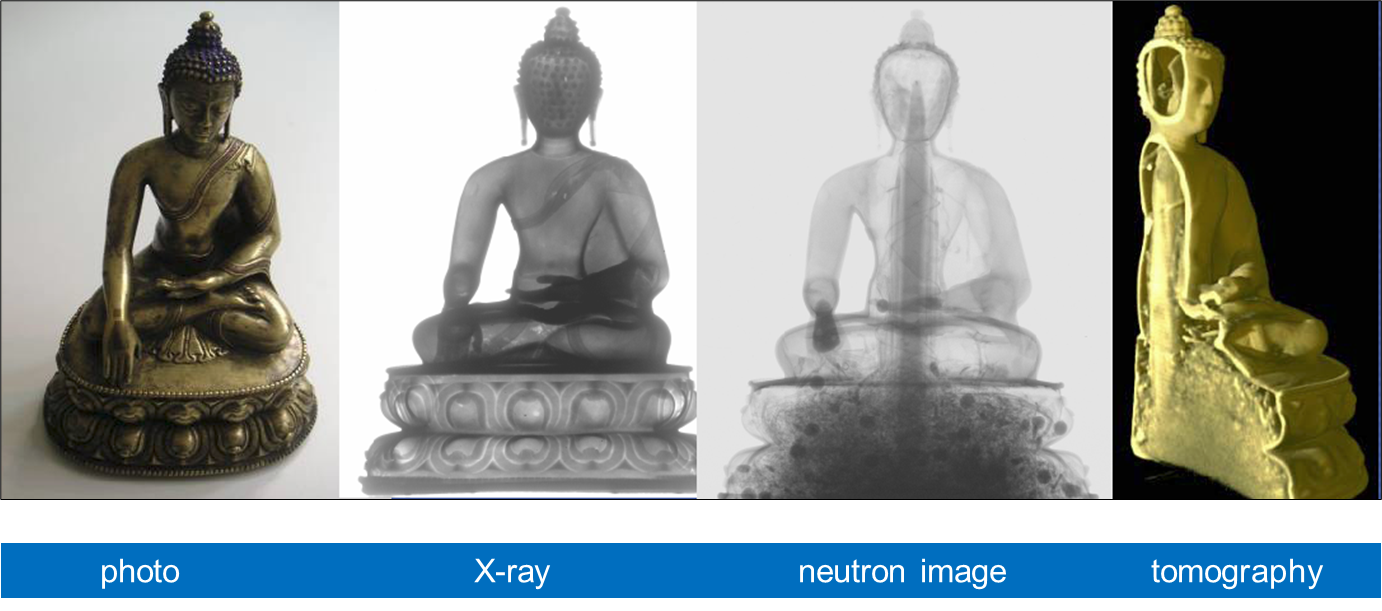
\includegraphics[width=0.7\linewidth]{img/Zobrazování.png}
    \caption{Příklady prosvícení neutrony.}
    \label{fig:Zobra}
\end{figure}

\begin{figure}
    \centering
    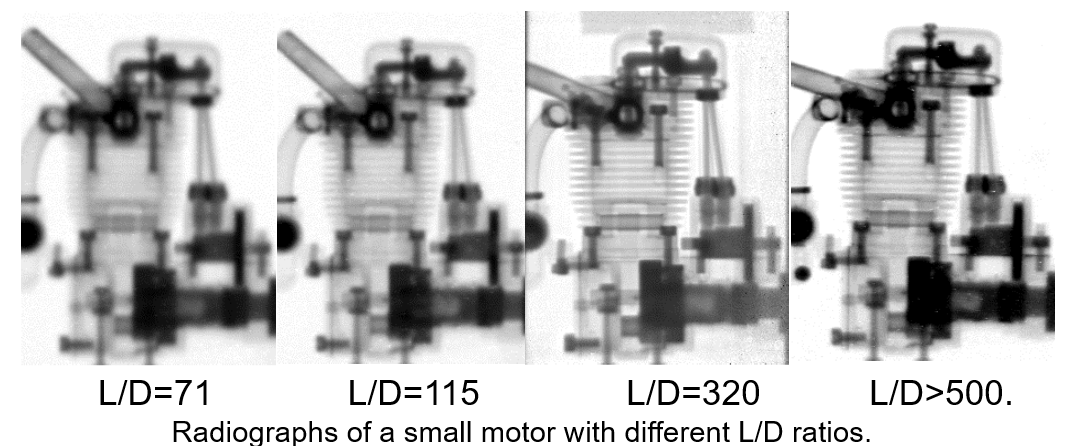
\includegraphics[width=0.5\linewidth]{img/RozlišeníPodleLD.png}
    \caption{Rozlišení podle L/D}
    \label{fig:enter-label}
\end{figure}

\subsection{Rozptylové reakce}

Rozptylové aplikace jsou založeny na částicově-vlnové dualitě neutronů. Zkoumání materiálu je založeno především na koherentním rozptylu neutronů. Tepelné neutrony mají vlnovou délku podobnou meziatomovým vzdálenostem, díky tomuto jevu je možné určovat vzdálenosti mezi jednotlivými atomy. Neutrony nemají náboj, proto se dostanou snáze do vnitřních struktur materiálů. 

Příkladem rozptylových aplikací je neutronová difrakce -- jedná se o pružný koherentní rozptyl, který se řídí Braggovým zákonem. Dalším příklady jsou rozptyl do malých úhlů (SANS -- small angle neutron scattering) a zpětný rozptyl (back scattering). 

\begin{figure}[H]
    \centering
    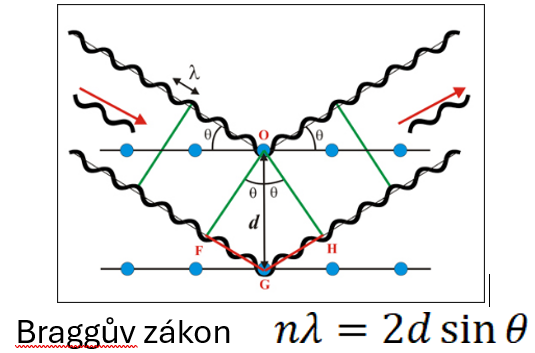
\includegraphics[width=0.5\linewidth]{img/Braggův zákon.png}
    \caption{Braggův zákon.}
    \label{fig:enter-label}
\end{figure}

Rozptylové aplikace se používají především v oblasti materiálového výzkumu, jako jsou fyzika a chemie kondenzovaných látek, nanotechnologie, věda o polymerech, výzkum udržitelné energie, senzory a chytré materiály atd.

Svazky můžou být vyvedeny i mimo hlavní budovu rekatoru. 

\begin{figure}[H]
    \centering
    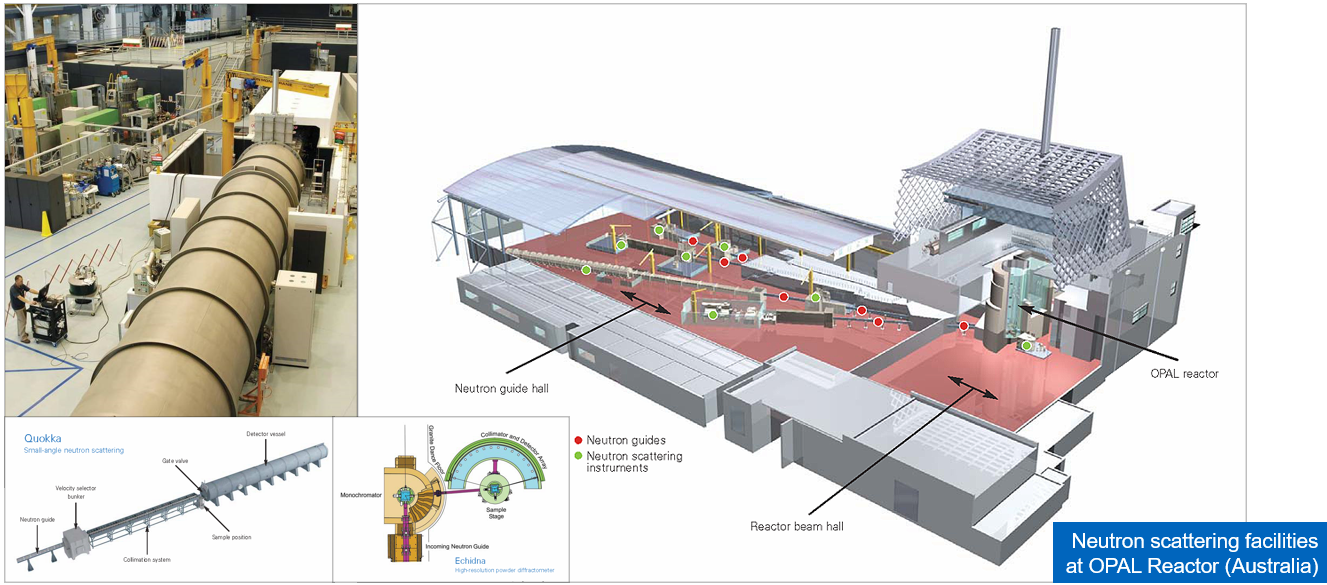
\includegraphics[width=0.75\linewidth]{img/OPALScattering.png}
    \caption{OPAL Scattering}
    \label{fig:enter-label}
\end{figure}

\subsection{Borová záchytová terapie}

Borová záchytová terapie je určena především k léčbě nádorů hlavy a krku. Je založena na interakci neutronového svazku s $^{10}$B, který je umístěn do speciálního roztoku. Ten je absorbován nádorem, který je poté bombardován svazkem neutronů. Dochází k (n, $\alpha$) reakci a vzniklé alpha záření poškozuje okolní nádorovou tkáň. 

Klinické studie byly provedeny v řadě zemí: Japonsko, Spojené státy americké, Finsko, Švédsko, Česká republika, Argentina. Současný trend je přesouvat léčbu z výzkumných reaktorů na urychlovače, které mohou být umístěny přímo v nemocnicích a poskytnou příjemnější prostředí pro pacienty. 

\subsection{Vzdělávání a školení}

Výzkumné reaktory poskytují vynikající možnosti pro vzdělávání i školení. Jsou vhodné pro výuku studentů na všech úrovních univerzitního vzdělávání a pro školení odborníků z průmyslu a výzkumných institucí. Mezi klíčové skupiny, které mohou těžit z výcviku na výzkumných reaktorech, patří:

\begin{itemize}
    \item Personál jaderných elektráren
    \item Personál výzkumných reaktorů
    \item Inspektoři regulačních orgánů
    \item Inspektoři radiační ochrany z různých organizací
    \item Hasičské záchranné sbory
\end{itemize}

Výzkumné reaktory jsou obzvláště vhodné pro jaderné vzdělávání studentů na všech třech úrovních akademického vzdělání. Výzkumné reaktory podporují široké spektrum studijních programů.

Výzkumné reaktory slouží také jako cenný nástroj pro zapojení veřejnosti, umožňují exkurze a návštěvy, které podporují porozumění jaderné vědě a technologii.
\section[Konstrukce a provoz výzkumných reaktorů]{Konstrukce a provoz výzkumných reaktorů}
\section[Bezpečnost výzkumných reaktorů]{Bezpečnostní aspekty provozu výzkumných reaktorů}

% \section[Měření reaktivity]{Metody měření reaktivity a stanovení charakteristiky absorpční tyče}


% \section[Měření rozložení hustoty toku]{Měření rozložení hustoty toku neutronů a jejich spektra v aktivní zóně reaktoru}
% \section[Kritický experiment]{Kritický experiment}

\subsection{Kritický stav}

Kritický stav jaderného reaktoru je označení stavu reaktoru, ve kterém je podíl množství neutronů v aktuální a předcházející generaci roven jedné: 

\begin{equation}
    \boxed{ k_\text{ef} = \frac{N_\text{i}}{N_\text{i-1}} = 1.}
\end{equation}

Přiblížení ke kritickému stavu lze provést různými způsoby v závislosti na konstrukčním řešení jaderného reaktoru. Nejčastěji se na jaderných reaktorech uvažuje vysouvání nebo zasouvání absorpčních tyčí, nebo změna koncentrace absorbátoru v chladivu (kyseliny borité H$_3$BO$_3$). Na výzkumných reaktorech se lze setkat i s dalšími způsoby, mezi něž se řadí:

\begin{itemize}%[noitemsep]
    \item přidávání nebo odebírání štěpného materiálu, tj. změna množství štěpného materiálu (viz regulace na EDU),
    \item změna úrovně vodní hladiny, tj. změna množství moderátoru (myslím, že to umí i LR0; případně změnit rychlost průtoku, čímž se změní teplota a hustota moderátoru, viz BWR reaktory),
    \item přibližování nebo oddalování reflektoru (výzkumný reaktor v SSSR nebo nějaké vesmírné reaktory).
\end{itemize}

Kritického stavu reaktoru je dosahováno při každém uvádění reaktoru do provozu. Změna výkonu je také v podstatě krátkodobým odchýlením od kritického stavu a jeho opětovným dosažením. Tento postup se ale vždy odehrává na známém uspořádání AZ. Pokud se spouští reaktor po změnách konfigurace AZ nebo úplně poprvé, je dosažení kritického stavu spojeno vždy s jistým prvkem neurčitosti. Ani zkušenost operátorů a kontrolních fyziků, ani precizní fyzikální výpočty nemohou zaručit přesné určení kritické velikosti AZ, poloh absorpčních tyčí nebo přesného množství absorbátoru při kritickém stavu reaktoru. Proto se na většině reaktorových provozů provádí tzv. \textbf{kritický experiment}, který k minimalizaci neurčitostí při dosažení prvního kritického stavu využívá jak výsledky neutronově-fyzikálních výpočtů, tak i měření v průběhu experimentu. V případě reaktoru VR-1 se jedná o jeden z nejnáročnějších experimentů, proto je jeho provedení zohledněno mimo jiné i v limitech a podmínkách. 

%Přiblížení ke kritickému stavu lze provést různými způsoby v závislosti na konstrukčním řešení jaderného reaktoru. Nejčastěji se na jaderných reaktorech k tomuto účelu používá vysouvání nebo zasouvání absorpčních tyčí, nebo změna koncentrace absorbátoru v chladivu, tj. změnu množství absorbátoru v AZ.

\subsubsection{Metoda inverzní četnosti}

Pokud bychom byli schopni měřit koeficient podkritického násobení $M$, lze kritický stav reaktoru predikovat z převrácené hodnoty $M$, respektive její závislosti na parametru $x$ (množství paliva, poloha absorpčních tyčí nebo množství moderátoru), který ovlivňuje hodnotu $k_\text{ef}$. Ze závislosti podílu $1/M$ na parametru $x$ můžeme pomocí extrapolace zjistit, pro jakou hodnotu $x$ bude podíl $1/M$ \textbf{roven nule a v tomto bodě můžeme očekávat kritický stav reaktoru}.

\begin{equation*}
    \lim_{m \to \infty} S \cdot \frac{1 - k_\text{ef}^m}{1 - k_\text{ef}} = \frac{S}{1 - k_\text{ef}} \rightarrow M = \frac{S}{S \cdot (1 - k_\text{ef})} = \frac{1}{1 - k_\text{ef}} \rightarrow \frac{1}{M} = 1 - k_\text{ef}
\end{equation*}

Při reaktorových experimentech získáváme údaje, které charakterizují hustotu neutronů. Jak zjistíme dále, lze nahradit koeficient podkritického násobení $M$ odezvou detektoru v daném místě AZ reaktoru. Předpokládejme, že přibližování ke kritickému stavu začíná od výchozího stavu AZ, který bude označen indexem $0$, dále označme všechny následující stavy AZ indexem $i$. Hustota toku neutronů pro výchozí stav AZ a stav AZ v kroku $i$ je výsledkem násobení v podkritickém reaktoru s externím zdrojem neutronů a lze ji vyjádřit následujícími vztahy:

\begin{equation*}
    \phi_0 \approx \frac{S}{1-k_{\text{ef},0}} \hspace{3cm}\phi_i \approx \frac{S}{1-k_{\text{ef},i}},
\end{equation*}

kde $\phi_0$ resp. $\phi_i$ je hustota toku neutronů ve výchozím resp. aktuálním stavu AZ, $k_{\text{ef},0}$ resp. $k_{\text{ef},i}$ je efektivní koeficient násobení pro výchozí resp. aktuální stav AZ a $S$ značí externí zdroj neutronů.

Z poměru hustot toku neutronů ve výchozím a aktuálním stavu lze s určitou přesností stanovit aktuální hodnotu efektivního koeficientu násobení jako:

\begin{equation*}
    \frac{\phi_0}{\phi_i} = \frac{S}{1 - k_{\text{ef},0}} \cdot \frac{1 - k_{\text{ef},i}}{S} = \frac{1 - k_{\text{ef},i}}{1 - k_{\text{ef},0}}= C \cdot (1-k_{\text{ef},i}),
\end{equation*}

kde $C=\dfrac{1}{1-k_\text{ef,0}}$ je nějaká konstanta pro výchozí stav (je úplně jedno, že ji neznáme).

Hustota toku neutronů je úměrná naměřeným četnostem (CR$_0$ a CR$_i$) získaným z detektorů, pak lze psát:

\begin{equation*}
    \frac{CR_0}{CR_i} \approx \frac{\phi_0}{\phi_i} \approx C \cdot (1-k_{\text{ef},i}).
\end{equation*}

Tedy pro kritický stav ($k_{\text{ef},\text{krit}} = 1$) musí platit $\frac{CR_0}{CR_i} = 0$.

\subsubsection{Experimentální predikce kritického stavu}

Ve výchozím stavu $x_0$ ($k_{\text{ef},0} <$  1) určíme počáteční četnost CR$_0$. Je logické, že první hodnota charakterizující inverzní četnost je rovna jedné. Po naměření je tyč posunuta do polohy $x_1$ a opět určen poměr CR$_0$/CR$_1$. Obě hodnoty jsou vyneseny do grafu závislosti CR$_0$/CR$_i$ na poloze $x_i$.

Extrapolací těchto dvou bodů je zjištěn první odhad kritického stavu ($x_i^\text{E}$). Regulační tyč je poté vysouvána z AZ po krocích délky odpovídající vztahu: (vztah mi říká jak moc mám v dalším kroku tyč vysunout)

\begin{equation} \label{eq:KS}
    x_{i+1} =x_i+\frac{1}{2} \cdot \{\text{min}(x_\text{E},x_\text{V}) - x_i\},
\end{equation}

kde hodnota 1/2 je volena z čistě konzervativních důvodů, $x_\text{E}$ značí experimentálně určenou polohu regulační tyče vždy ze dvou posledních bodů a $x_\text{V}$ značí polohu \textbf{kritického stavu} určenou výpočetním programem.

Tato iterace je prováděna do té doby, dokud se hodnota CR$_0$/CR$_i$ $\approx 0,2$. Poté se reaktor nachází v blízkosti kritického stavu a opětovnou extrapolací poslední 2-3 hodnot lze určit předpokládanou polohu regulační tyče pro kritický stav.

Významnou roli hraje vzdálenost neutronového zdroje od detektoru, vzdálenost detektoru od místa, v němž je měněn (ovlivňován) koeficient násobení
a samozřejmě způsob, jakým závisí změna koeficientu násobení na změně proměnného
parametru $x_i$.

\begin{figure}[H] 
    \centering
    \includegraphics[scale=0.7]{img/KritickýExperiment.png}
    \caption{Závislost CR$_0$/CR$_i$ na poloze $x_i$.}
    \label{SNM}
\end{figure}

Vtipný je, že tenhle jednoduchý a old-style způsob se skutečně využívá i na velkých reaktorech (ne jenom VR-1), pouze to nedělají ručně, ale mají na to prográmek (on stačí Excel). Kamarád byl na stáži na elektrárně, kde ho nechali to samé rýsovat na milimetrový papír a nezávisle ho kontrolovali vlastním prográmkem, a to bylo v rámci skutečného najíždění nové vsázky.

\subsection{Kritický experiment na VR-1}
V rámci předmětu 17KEX, při němž se sestavuje "nová" AZ se po sestavení základní vsázky postupuje následovně:
\begin{itemize}
    \item Přidá se další PČ a provádí se měření reaktivity v DKP a HKP (dokud to jde, aby reaktor nebyl kritický) s využitím SNM detektorů ve 3 různých pozicích a PMV kanálů. Všechny výsledky se srovnávají s numericky vypočtenými hodnotami a kontroluje se jejich shoda. 
    \item Po složení celé AZ se postupně vytahují bezpečnostní, experimentální a jedna regulační tyč do HKP (v každém kroku se provádí měření).
    \item Nakonec se vytahuje (BÚNO R2) po krocích dané rovnicí \eqref{eq:KS} a dosahuje se KS.
\end{itemize}

% \section[Prostorové a energetické rozložení hustoty toku, spektrální indexy]{Prostorové a energetické rozložení hustoty toku neutronů v aktivní zóně reaktoru a spektrální indexy}


% \section[Měření kinetických parametrů]{Kinetické parametry reaktoru, zpožděné neutrony, jejich vlastnosti, vliv na provoz reaktoru a určování jejich parametrů}

\subsection{Zpožděné neutrony}

Kinetika a dynamika jaderného reaktoru v průběhu jeho provozu (především při přechodových procesech) je do značné míry udávána zpožděnými neutrony. Znalost parametrů zpožděných neutronů je velmi významná nejen při návrhu, ale i vlastním provozu jaderných reaktorů. Zpožděné neutrony lze využít také jako analytický nástroj, pomocí něhož lze přesněji určit obohacení, respektive hmotnost štěpného materiálu.

Z hlediska řízení reaktivity platí, že nikdy nesmí dojít ke kritičnosti na okamžitých neutronech, jelikož se tím drasticky (až o několik řádů) sníží perioda reaktoru, viz otázky FJR. Rovněž více o kinetických parametrech reaktoru je k dohledání v otázkách FJR, případně ve wikiSkriptech z KIDu

\subsubsection{Vznik a vlastnosti zpožděných neutronů}

Štěpení spočívá v rozdělení jádra (např. $^{235}\text{U}$) na dva nebo více úštěpků s hmotnostmi a atomovými čísly podstatně menšími než u výchozího jádra. V prvním stádiu štěpné reakce dochází k pohlcení neutronu, přičemž vznikne jádro $^{236}\text{U}$ ve vzbuzeném stavu:

\[
^{235}_{92}\text{U} + \text{n} \rightarrow ^{236}_{92}\text{U}^*
\]

Takto vzniklé jádro může emitovat gama záření a přejít tak do základního stavu nebo může dojít k jeho rozštěpení. 

Produkty štěpení mají příliš vysoký poměr počtu neutronů k počtu protonů a jsou tedy nestabilní. Proto téměř všechny produkty štěpení jsou radioaktivní a dochází u nich nejčastěji k rozpadu $\beta^-$ se spojeným zářením gama. Radioaktivní bývají i přímé produkty rozpadu, u nichž může opět docházet k rozpadu $\beta^-$, než vznikne stabilní jádro. Délka rozpadových řad bývá různá, v průměru procházejí produkty štěpení třemi rozpadovými stádii, než se utvoří stabilní jádro. V některých případech vede rozpad $\beta^-$ jádra, které se nachází ve vzbuzeném stavu, k uvolnění neutronu. Jelikož energie vázaného neutronu je nižší než vazbová energie neutronu v jádře, pak je určitá pravděpodobnost, že dojde k emisí neutronu a vzniku stabilního jádra. Uvolněný neutron se nazývá zpožděným neutronem. Zpoždění je dáno pouze poločasem rozpadu produktu štěpení, který je nazýván prekurzorem, jelikož k uvolnění neutronu dochází až po předchozím rozpadu jeho jádra.

Obecně lze zapsat vznik zpožděného neutronu následujícím předpisem:

\[
^A_Z\text{X} \xrightarrow{\beta^-} {}^{A}_{Z+1}\text{Y} \rightarrow ^{A-1}_{Z+1}\text{Y} + \text{n}
\]

kde:

\begin{itemize}%[noitemsep]
    \item[$-$] $^A_Z\text{X}$ je produkt štěpení, jádro nazývané prekurzor neboli předchůdce mateřského jádra,
    \item[$-$] $^{A}_{Z+1}\text{Y}$ je jádro nazývané emitor neboli mateřské jádro,
    \item[$-$] $^{A-1}_{Z+1}\text{Y}$ je výsledné jádro.
\end{itemize}

Na Obrázku \ref{SNM} je znázorněno rozpadové schéma typického prekurzoru $^{87}\text{Br}$. Izotop $^{87}\text{Br}$ hraje významnou roli v případě odstavení jaderného reaktoru, kdy odezní vliv okamžitých a krátkodobě žijících zpožděných neutronů. V tomto případě je populace neutronů v AZ určována především rozpadem $^{87}\text{Br}$. Jak vyplývá z obrázku, přibližně 30~\% jader $^{87}\text{Br}$ přechází rozpadem $\beta^-$ na $^{87}\text{Kr}$, který se nachází v základním stavu, zatímco 70~\% jader přechází rozpadem $\beta^-$ na $^{87}\text{Kr}$ ve vzbuzeném stavu ($^{87}\text{Kr}^*$). Z těchto 70~\% přechází přibližně 20~\% jader $^{87}\text{Kr}^*$ izomerickým přechodem do základního stavu. Zbýlá jádra ($^{87}\text{Kr}^*$) se dostávají do základního stavu přímou emisí neutronu. Tím vzniká zpožděný neutron. Prekurzorem je tedy $^{87}\text{Br}$, který opět rozpadem $\beta^-$ přechází na již stabilní $^{87}\text{Sr}$. Zpožděný neutron není emitován přímo jádrem $^{87}\text{Br}$, ale dceřiným produktem ve vzbuzeném stavu ($^{87}\text{Kr}^*$).

\begin{figure}[H] 
    \centering
    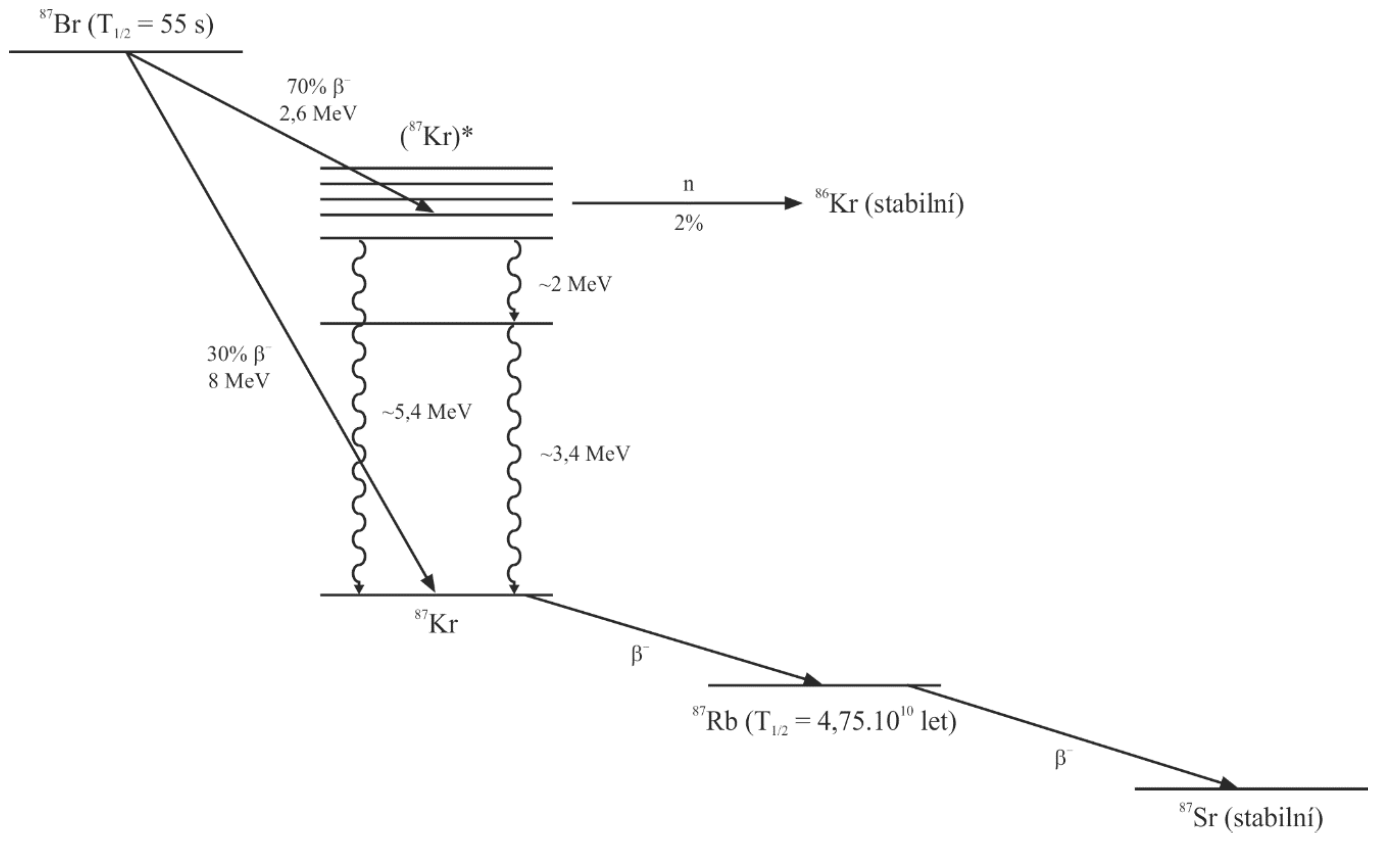
\includegraphics[width=0.8\textwidth]{img/ZpožděnéNeutrony.png}
    \caption{Rozpadové schéma $^{87}$Br.}
    \label{SNM}
\end{figure}

V současnosti bylo identifikováno téměř 400 prekurzorů zpožděných neutronů. Nejdéle žijícími jsou $^{91}\text{Rb}$ a $^{87}\text{Br}$ s poločasem rozpadu 58,4~s, respektive 55,6~s, zatímco $^{102}\text{Rb}$ a $^{101}\text{Rb}$ jsou krátkodobě žijící prekurzory s poločasem rozpadu 37~ms, respektive 32~ms. Jelikož k emisi neutronu dochází bezprostředně po rozpadu prekurzoru, řídí se časové zpoždění, s nímž se emitované neutrony objevují, zákony radioaktivního rozpadu těchto jader.

Jelikož prekurzorů je moc, tak se pro optimalizaci výpočtů prekurzory slučují do několika skupin, přičemž každá skupina je charakteristická jedním středním poločasem rozpadu a jedním společným kumulativním výtěžkem. Čím více skupin, tím přesnější výpočet, ale tím složitější a zdlouhavější výpočet. Pro první přiblížení stačí použít 1-2 skupiny, lepší kódy aplikují 6-8 skupin (záleží na knihovně, např. ENDF/B má 6 skupin a JEFF 8 skupin).

\begin{table}[H]
    \centering
    \begin{tabular}{@{}ccc@{}}
    \toprule
    Skupina & Prekurzor                              & T$_{1/2}$ (s) \\ \midrule
    1       & $^{87}$Br, $^{142}$Cs                  & 55,72         \\
    2       & $^{137}$I, $^{88}$Br                   & 22,72         \\
    3       & $^{138}$I, $^{89}$Br                   & 6,22          \\
    4       & $^{139}$I, $^{(93, 94)}$Kr, $^{143}$Xe & 2,30          \\
    5       & $^{140}$I, $^{145}$Cs                  & 0,61          \\
    6       & Br, Rb, As…                            & 0,23          \\ \bottomrule
    \end{tabular}
\end{table}

Kumulativní výtěžek označovaný jako $\beta$ se pohybuje v desetinách procenta, záleží, který izotop se štěpí. Pro $^{235}$U je to asi 0,7 \%, pro izotopy Pu je to méně. Proto jsou MOXové vsázky citlivější na změnu výkonu.

Kromě výše uvedených parametrů je důležitou charakteristikou zpožděných neutronů i jejich energie. Ta se pohybuje pro jednotlivé skupiny zpožděných neutronů v rozmezí od 200~keV do 700~keV. Porovnáme-li tento rozsah energií se střední energií okamžitých neutronů (2,2~MeV), je zřejmé, že zpožděné neutrony musí v rámci zpomalovacího procesu projít menším rozsahem energií než neutrony okamžité. Je nižší pravděpodobnost, že dojde k jejich ztrátě v důsledku úniku nebo parazitické absorpce, než v případě okamžitých neutronů. Naopak u okamžitých neutronů je vyšší pravděpodobnost, že vyvolají štěpení ve vyšší oblasti energií (např. na $^{238}\text{U}$). Tyto dva efekty mají tendenci působit navzájem proti sobě, nicméně je obvykle mezi nimi určitý, i když mírný, rozdíl. V důsledku toho se definuje tzv. efektivní podíl zpožděných neutronů $\beta_\text{ef}$, který zohledňuje rozdílnou energii zpožděných neutronů oproti neutronům okamžitým a tím i jejich význam v procesu štěpení. Je tedy závislý na typu reaktoru, moderaci apod.

\subsubsection{Emise zpožděných neutronů}

Emise zpožděných neutronů je spojena se vznikem a aktivitou jejich jednotlivých mateřských jader. Vznik konkrétního prekurzoru zpožděných neutronů v průběhu ozařování můžeme popsat bilanční rovnicí ve tvaru:

\[
\frac{dN_i}{dt} = Y_C \cdot \Sigma_f \cdot \Phi - \lambda_i \cdot N_i
\]

kde:

\begin{itemize}%[noitemsep]
    \item[$-$] $N_i$ je počet mateřských jader zpožděných neutronů $i$-tého druhu,
    \item[$-$] $Y_C$ je kumulativní výtěžek mateřských jader zpožděných neutronů ze štěpení,
    \item[$-$] $\Sigma_f$ je reakční rychlost pro štěpení,
    \item[$-$] $\Phi$ je hustota toku neutronů,
    \item[$-$] $\lambda_i$ je rozpadová konstanta mateřských jader zpožděných neutronů.
\end{itemize}

Pro jednoduchost je zanedbán záchyt neutronů mateřskými jádry zpožděných neutronů. Tuto rovnici lze jednoduše řešit pro $N_i$ jako funkci času ozařování:

\[
N_i(t) = \frac{Y_C \cdot \Sigma_f \cdot \Phi}{\lambda_i} \cdot \left(1 - e^{-\lambda_i t}\right).
\]

Abychom získali emisi zpožděných neutronů (tj. zdrojový člen), je nutné vynásobit obě strany rozpadovou konstantou $\lambda_i$. Za předpokladu, že mateřské jádro prochází rozpadem vedoucím k emisi neutronu $P_i$, předpokládáme-li, že druhů mateřských jader a ozářovacích časů je $t_\text{irr}$, pak počet zpožděných neutronů emitovaných v čase $t$ po ukončení ozařování bude:

\[
N_{DN}(t) = \sum_{i=1}^{m} P_i \cdot Y_C \cdot \Sigma_f \cdot \Phi \cdot (1 - e^{-\lambda_i t_\text{irr}}) \cdot e^{-\lambda_i t}.
\]

V souladu s teorií lze zpožděné neutrony rozdělit do šesti skupin podle typických mateřských jader a vztah přepsat na tvar:

\[
N_{DN}(t) = \sum_{i=1}^{6} a_i \cdot (1 - e^{-\lambda_i t_\text{irr}}) \cdot e^{-\lambda_i t},
\]

kde $a_i$ je zastoupení $i$-té skupiny zpožděných neutronů. Bude-li provedeno pouze krátkodobé ozařování (např. neutronovým pulzem), pak rovnice nabývá tvar:

\begin{equation}
    \boxed{N_{DN}(t) = \sum_{i=1}^{6} a_i \cdot e^{-\lambda_i t}.}
\end{equation}

Je-li doba ozařování dostatečně dlouhá ($t_\text{irr} \gg \tau_i$), přechází rovnice na tvar:

\begin{equation}
    \boxed{N_{DN}(t) = \sum_{i=1}^{6} a_i \cdot (1 - e^{-\lambda_i t}).}
\end{equation}

\subsubsection{Stanovení poločasu rozpadu prekurzorů zpožděných neutronů}

V případě, že bychom chtěli určit parametry jednotlivých skupin zpožděných neutronů a celkovou emisi rozdělit na individuální rozpadové křivky, je nutné aplikovat na analyzovaná data metody nelineární regrese. Takováto úloha není jednoduchá a pro její řešení jsou běžně používány sofistikované softwarové nástroje pro analýzu dat. Nicméně úloha se výrazně zjednoduší, pokud se bude jednat o hledání parametrů pouze jedné exponenciální funkce. Toho lze dosáhnout, pokud si uvědomíme, že platí $\lambda_1 \ll \lambda_2 \ll \dots \ll \lambda_6$ a $e^{-\lambda_1 t} \gg e^{-\lambda_2 t} \gg \dots \gg e^{-\lambda_6 t}$. Po dostatečně dlouhé době, která vede k rozpadu předchozích skupin zpožděných neutronů, můžeme vztah aproximovat pouze jednou exponenciální funkcí odpovídající nejdéle žijící skupině zpožděných neutronů:

\[
N_{DN}(t) = a_1 \cdot e^{-\lambda_1 t}
\]

Tuto funkci lze linearizovat použitím přirozeného logaritmu:

\[
\ln N_{DN}(t) = \ln a_1 - \lambda_1 \cdot t
\]

díky čemuž můžeme jednoduše určit parametry $a_1$ a $\lambda_1$. Takto získanou teoretickou emisi odečteme od celkové emise:

\[
N_{DN}(t) - a_1 \cdot e^{-\lambda_1 t}
\]

Tento rozdíl pak představuje četnost emise pro zbývající skupiny zpožděných neutronů (2 až 6), z něhož můžeme na základě výše popsané úvahy určit parametry zpožděných neutronů druhé skupiny ($a_2$ a $\lambda_2$). Tímto způsobem bychom pokračovali až k určení parametrů skupiny zpožděných neutronů s nejkratší dobou života ($a_6$ a $\lambda_6$).

Problém nastane u krátkodobých skupin (5 a 6), jelikož jejich poločas rozpadu je tak malý, že než dojde k měření, tak se většina prekurzorů rozpadne.

\subsubsection{Určování množství štěpného materiálu}

Z předchozí teorie je zřejmé, že celkový počet zpožděných neutronů emitovaných ozářeným štěpným materiálem závisí na počtu štěpení, což je samozřejmě spjato s množstvím jader ve štěpném materiálu. Tudíž lze využít této závislosti k určení vybraných vlastností zkoumaného vzorku, jako je množství, respektive obohacení štěpného materiálu ve vzorku.

Metoda určování množství nebo obsahu štěpného materiálu ve zkoumaném vzorku na základě detekce zpožděných neutronů je rychlá, nedestruktivní, přesná a velmi citlivá analytická metoda. Je založena na ozáření vzorku obsahujícího štěpný materiál neutrony a následné detekci zpožděných neutronů, které jsou emitovány tímto vzorkem. Množství nebo obsah štěpného materiálu ve zkoumaném vzorku je pak určená na základě porovnání intenzity zpožděných neutronů emitovaných tímto vzorkem se vzorky (standardy), u nichž je známo množství nebo obsah štěpného materiálu (za pomoci trojčlenky).

Předpokládejme zjednodušeně, že celkový počet zpožděných neutronů emitovaných ozářeným vzorkem a detekovaný detekčním systémem je roven součtu četností získaných za dobu detekce $(t_\text{end} - t_\text{start})$. Pak lze počet zpožděných neutronů $N_X$ odpovídající neznámému vzorku a počet zpožděných neutronů $N_\text{ST}$ odpovídající standardu, určit na základě následujících vztahů:

\[
N_X = \sum_{i = t_\text{start}}^{t_\text{end}} CR_{X,i}, \quad N_\text{ST} = \sum_{i = t_\text{start}}^{t_\text{end}} CR_{\text{ST},i},
\]

kde $CR_{X,i}$ a $CR_{\text{ST},i}$ jsou četnosti získané v $i$-tém časovém kroku detekčního systému pro neznámý vzorek a standard.

Je-li odezva detekčního systému na pozadí rovna:

\[
N_\text{BG} = \sum_{i = t_\text{start}}^{t_\text{end}} CR_{\text{BG},i},
\]

pak platí pro závislost počtu zpožděných neutronů produkovaných standardem na jeho hmotnosti $m_\text{ST}$ následující úměra:

\begin{equation}
m_X = m_{ST} \cdot \frac{N_X - N_\text{BG}}{N_{ST}-N_\text{BG}}.
\end{equation}

Přesnější výslednou hodnotu $m_X$ neznámého vzorku získáme, pokud použijeme více než jeden standard se štěpným materiálem. V takovém případě je vhodné vynést do grafu závislost celkového počtu zpožděných neutronů na množství štěpného materiálu, proložit data vhodnou křivkou a získat její rovnici. Z rovnice lze pak určit neznámé množství štěpného materiálu ve zkoumaném vzorku. Nicméně je důležité, aby se všemi vzorky bylo nakládáno za stejných experimentálních podmínek (hustota toku neutronů, doba ozařování, doba transportu vzorku a doba detekce) a kromě toho musí mít vzorky podobnou geometrii.
% \section[Režimy a provoz neutronových detektorů]{Základní dělení, charakteristiky, provozní režimy a konfigurace provozních parametrů detektorů neutronů}

\subsection{Princip detekce neutronů}

Neutron je elektricky neutrální, proto pokud ho chceme detekovat, musíme postupovat nepřímo. Je potřeba neutron konvertovat na jinou nabitou částici (elektron, alfa, proton, ...), která se potom snáze detekuje. 

Detekce prostřednictvím sekundárních částic. Používají se detektory nabitých částic s konverzním materiálem naneseným na povrchu detektoru, někdy je konvertor přímo v aktivní části detektoru jako plyn, aby vznikající sekundární ionizující záření mohlo být bezprostředně detekováno. 

\subsubsection{Konvertor neutronů}

Konvertory neutronů představují klíčovou součást detektorů určených k měření neutronového záření. Jejich návrh a konstrukce musí splňovat následující požadavky.

\textbf{Požadavky na konvertor neutronů:}

\begin{itemize}
    \item \textbf{Velký účinný průřez:} Materiál použitý v konvertoru musí mít co největší účinný průřez pro jadernou reakci, při níž dochází ke konverzi neutronu.
    \item  \textbf{Dostupnost materiálu:} Nuklid použitý jako terč by měl být dostatečně zastoupen v přírodním izotopickém složení, nebo musí existovat cenově efektivní a účinný způsob získávání obohaceného materiálu.
    \item  \textbf{Energie uvolněná při reakci (Q-hodnota):} Energie uvolněná při konverzní jaderné reakci (Q) je důležitým parametrem. Vyšší hodnota Q umožňuje snazší potlačení doprovodného gama záření.
\end{itemize}

\textbf{Požadavky na konstrukci detektoru:}

Detektor musí být navržen tak, aby částice vzniklé při konverzní reakci odevzdaly celou svou kinetickou energii v jeho aktivním objemu. Aktivní délka detektoru musí být proto dostatečná, aby zajistila kompletní absorpci energie.

\textbf{Typy konvertorů podle skupenství:}

\begin{itemize}
    \item  \textbf{Plynné konvertory:} Ionizační a proporcionální plynové komory využívající plynný konvertor ($^3$He, $^{10}$BF$_3$).
    \item  \textbf{Kapalné konvertory:} Kapalné scintilátory.
    \item \textbf{Pevné konvertory:} 
    \begin{itemize}
        \item  Plynové komory s pevným konvertorem (např. s vrstvou $^{10}\text{B}$, $^{235}$U).
        \item  Scintilátory ($^6$LiI(Eu)).
        \item  Polovodičové detektory (konvertor nanesený nad PN přechodem).
        \item  Termoluminiscenční detektory (z $^6$LiF, dochází k excitaci elektronů, které zamrznou v mřížce. Po následném ohřátí se uvolní a změří).
        \item  Plastové nebo emulzní detektory zaznamenávající stopy neutronů.
    \end{itemize}
\end{itemize}

Citlivost detektoru závisí na hustotě atomů v konvertoru (počet atomů na $\text{cm}^3$). Vyšší hustota atomů zvyšuje citlivost na neutrony, avšak zároveň i na gama záření. Proto nelze jednoznačně preferovat konkrétní skupenství materiálu konvertoru; volba závisí na specifických požadavcích konkrétní aplikace.

Většina detektorů má on-line odezvu, ale existují i detektory, které se musí později vyhodnotit (TLD, aktivační fólie). Účel měření neutronů může být:

\begin{itemize}
    \item fluence neutronů (neutronový tok),
    \item spektrometrie neutronů (mimo počtu částic zaznamenáváme i jejich energie),
    \item měření ekvivalentní dávky (dozimetry).
\end{itemize}
  
Nejčastější reakce pro konverzi neutronu na nabitou částici jsou:

\[
^3\text{He} + ^1\text{n} \to ^3\text{H} + ^1\text{p} + 0{,}765 \, \text{MeV} \ \ \text{(He detektor)}
\]
\[
^{10}\text{B} + ^1\text{n} \to ^7\text{Li} + \alpha + 2{,}3 \, \text{MeV} \ \ \text{(B detektor, scintilátor)}
\]
\[
^{10}\text{B} + ^1\text{n} \to ^7\text{Li} + \alpha + 2{,}8 \, \text{MeV} \ \ \text{(B detektor, scintilátor)}
\]
\[
^6\text{Li} + ^1\text{n} \to ^3\text{H} + \alpha + 4{,}79 \, \text{MeV}  \ \ \text{(Scintilátor)}
\]
\[
^{235}\text{U} + ^1\text{n} \to \text{FP} + 195 \, \text{MeV}  \ \ \text{(štěpné komory)}
\]

%Pro detekci sekundárních nabitých částic se používají plynové, scintilační, polovodičové a další detektory. Konvertorem je helium a bór v plynné fázi, resp. bór a lithium (Li) v pevné fázi. Největší problém detektorů neutronů je "odfiltrování" doprovodných jevů (zejména doprovodného $\gamma$).


Základem nastavení jak plynových, tak scintilačních detektorů je kombinace vysokého napětí (zesílení ve fotonásobiči) a zesílení (v zesilovači), tak aby výsledné pulsy měly amplitudu vhodnou pro další zpracování. Dále je nutno nastavit diskriminaci, tak aby optimálně splňovala následující kombinaci požadavků:

\begin{itemize}
    \item Malá změna (nestabilita) vysokého napětí by měla mít za následek minimální změnu četnosti pulsů. Tzn. nastavení v oblasti lokálního minima nebo aspoň ploché části amplitudového spektra.
    \item Pulsy iniciované neutrony by měly být minimálně potlačeny (nesnižovat citlivost).
    \item Maximálně by měly být potlačeny pulsy iniciované $\gamma$ zářením.
\end{itemize}

Diskriminace se stanovuje z amplitudového spektra, které je spolu s voltampérovou charakteristikou základními charakteristikami detekčního řetězce.

Důležitým parametrem detektoru je citlivost; ta určuje jeho použitelnost v praxi. Citlivostí detektoru rozumíme podíl četností na konci detekčního řetězce a toku neutronů. Citlivost záleží na spektru neutronů a k její stanovení je potřeba stanovit absolutní hustotu toku, tak spektrum neutronů. 

\subsection{Základní dělení}
Tohle jsou tak nějak všechny možné detektory neutronů, co jsem byl schopen najít:
\begin{itemize}
    \item Plynové detektory
    \item Scintilátory
    \item Polovodičové detektory
%    \item Diamantové detektory
    \item Samonapájecí detektory (SPD)
    \item Termoluminiscenční detektory (TLD)
    \item Aktivační detektory
%    \item Detektory stop v pevné fázi
\end{itemize}

\subsubsection{Plynem plněné detektory}

Plynem plněné detektory patří k nejrozšířenějším detektorům ionizujícího záření. Měří ionizaci produkovanou průchodem nabité částice prostředím. Jsou založeny na sběru iontů a elektronů vytvořených dopadajícím zářením v prostoru detektoru. Ionizace je způsobena buď přímo ionizujícím zářením ($\alpha$, $\beta$), nebo interakcí nepřímo ionizujícího záření (elektromagnetické, neutrony) s materiálem detektoru.

Plynové detektory měřící neutrony mají stejné uspořádání jako pro nabité částice. 
Konvertor je nuklid s vysokým účinným průřezem pro neutrony (nejčastěji $^1$H, $^3$He, $^6$Li, $^{10}$B, $^{235}$U). Nejčastěji je obsažen v plynové náplni nebo materiálu pokrývajícím stěny detektoru. Plynové detektory pracují nejčastěji v režimu ionizační komory nebo proporcionality.

Plynné prostředí plynové detektoru je řídké, což je výhoda z hlediska nízké citlivost ke $\gamma$ záření, ale na druhou stranu celková nižší účinnost kvůli menšímu účinnému průřezu.

\textbf{Borové komory:}

Borové komory využívají reakci $^{10}\text{B}(n, \alpha)$. Bór může být buď nanesený na vnitřní straně stěny komory, nebo použit jako plynová náplň BF$_3$. 

Reakce probíhají dle následujících rovnic:
\[
^{10}_5\text{B} + ^1_0\text{n} \rightarrow ^7_3\text{Li} + ^4_2\alpha \quad Q = 2{,}790\,\text{MeV} \quad (6\%)
\]
\[
^{10}_5\text{B} + ^1_0\text{n} \rightarrow ^7_3\text{Li}^* + ^4_2\alpha + \gamma(0{,}48\,\text{MeV}) \quad Q = 2{,}310\,\text{MeV} \quad (94\%)
\]

Příklady borových komor: SNM10, SNM12, používané například na reaktoru VR-1.

\textbf{Lithiové, heliové a gadoliniové komory}

Lithiové komory využívají reakci $^6\text{Li}(n, \alpha)$:
\[
^6_3\text{Li} + ^1_0\text{n} \rightarrow ^3_1\text{H} + ^4_2\alpha \quad Q = 4{,}784\,\text{MeV}
\]

Heliové komory pracují na základě reakce $^3\text{He}(n, p)$:
\[
^3_2\text{He} + ^1_0\text{n} \rightarrow ^3_1\text{H} + ^1_1\text{p} \quad Q = 0{,}764\,\text{MeV}
\]

Gadoliniové komory využívají reakce $^{157}\text{Gd}(n, \gamma)$ a vyznačují se velmi vysokou citlivostí. Pro jejich správnou funkci je nutná diskriminace gama záření.

\textbf{Štěpné komory:}

Štěpné komory pracují na základě štěpných reakcí s izotopy $^{235}\text{U}$, $^{233}\text{U}$ a $^{239}\text{Pu}$:
\[
^{235}\text{U}, ^{233}\text{U}, ^{239}\text{Pu} (n, f)
\]

Na povrchu štěpné komory je štěpný materiál, jako je $^{235}\text{U}$, $^{233}\text{U}$ nebo $^{239}\text{Pu}$, což je vhodné pro detekci tepelných neutronů. Štěpitelné materiály jako $^{238}\text{U}$ a $^{232}\text{Th}$ se používají pro detekci rychlých neutronů.

Je nutné diskriminovat vliv $\alpha$ záření ze štěpných nebo štěpitelných materiálů. Štěpné komory jsou citlivé také na gama záření, což vyžaduje další diskriminaci.

Příklad použití: Štěpné komory RJ1300 na reaktoru VR-1. Tyto komory zahrnují i miniaturizované varianty s průměrem jen 4,7 mm, které jsou vhodné pro vnitro-reaktorová měření (in-core měření).

\textbf{Klasifikace plynových detektorů}

\begin{figure}[H] 
    \centering
    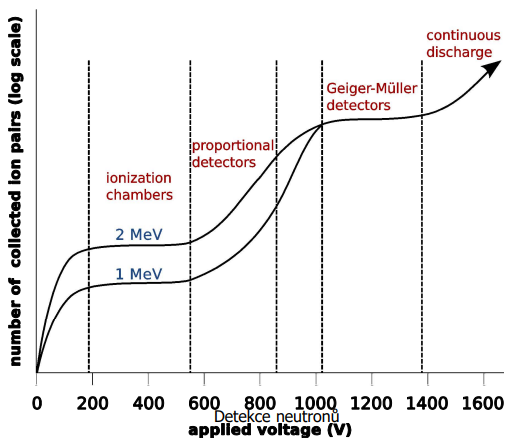
\includegraphics[width=0.5\textwidth]{img/KlasifikacePlynovýchDetektorů.png}
    \caption{Klasifikace plynových detektorů.}
    \label{fig:KlasifikacePlynovýchDetektorů}
\end{figure}

Klasifikace plynových detektorů zahrnuje několik typů, z nichž každý má své specifické vlastnosti a použití.

Ionizační komory pracují tak, že volba napětí zajistí, aby proud komorou nezávisel na napětí (nasycený proud). Odezva komory závisí i na energii záření a může být provozována impulzně i proudově.

Proporcionální detektory využívají vyšší napětí, které zvyšuje pravděpodobnost sekundární ionizace, plynového násobení a vzniku lavinového efektu. Počet iontových párů zde závisí na napětí, přičemž odezva je úměrná energii záření. Tento typ detektorů se využívá pro spektrometrii záření.

Oblast limitované proporcionality nastává při ještě vyšším napětí, které způsobí hromadění iontů u katody, což ovlivňuje elektrické pole v detektoru. Elektrony se snáze pohybují k anodě než těžké ionty ke katodě, což vytváří nelineární efekt, kdy výstupní signál není proporcionální k deponované energii. Tato oblast se dle literatury běžně nepoužívá.

Geiger-Müllerovy detektory fungují tak, že ionizující záření proniká okénkem do trubice, kde ionizuje plyn. Uvolněné elektrony jsou urychlovány k anodě, zatímco kladné ionty směřují ke katodě. Následná lavinová ionizace vede k vzniku volných nosičů náboje. Tento proces převyšuje rekombinaci, což umožňuje vznik výboje. Použití zhášedla (např. etylen, halogen) omezuje trvání výboje na mikrosekundy, což umožňuje detekci impulzů v rozsahu $10^4$ až $10^5$ za sekundu.

Koronové detektory nejsou schopny registrovat záření s nízkou ionizační schopností, jako je záření $\beta$ nebo $\gamma$. Při normálním režimu je v koronové vrstvě ionizovaný plyn, který vytváří koronový proud vedoucí ke vzniku milivoltových impulsů. Silně ionizující částice, jako jsou částice $\alpha$, mohou vytvořit impulsy s amplitudou až 300~mV. Tento typ detektorů zachovává úměrnost mezi energií částice a amplitudou impulsu.

Jiskrové detektory pracují ve vzduchu při normálním tlaku. Mezi katodou a anodou je aplikováno stejnosměrné napětí několik kilovoltů. Ionizující částice, která vstoupí mezi elektrody, způsobí jiskrový výboj, který může být detekován jako impuls napětí nebo fotograficky jako jiskra. Moderní jiskrové detektory mají velmi krátké impulsy (řádově $10^{-9}$~s), což je jejich hlavní předností oproti Geiger-Müllerovým detektorům.

Každý z těchto detektorů má specifické výhody a použití, a jejich volba závisí na požadavcích konkrétní aplikace.

\subsubsection{Scintilační detektory}

Scintilační detektory představují zařízení pro detekci ionizujícího záření, které fungují na principu excitace elektronu do vyššího energetického stavu zářením. Návrat elektronu do základního stavu je doprovázen emisí světelného záblesku.

Proces detekce probíhá ve dvou krocích:

\begin{itemize}
    \item Ionizující záření je převedeno na viditelné nebo ultrafialové světlo pomocí scintilačního materiálu (krystalu). Při absorpci záření dochází k excitaci elektronů krystalu, které následně při de-excitaci emitují fotony viditelného světla.
    \item  Viditelné světlo je detekováno a převedeno na elektronický signál pomocí zařízení, jako je fotonásobič.
\end{itemize}

Používané scintilační materiály zahrnují organické látky, jako jsou naftalen a antracen, i anorganické látky, například NaI, CsI nebo BaF$_2$. Každý materiál má specifické vlastnosti, které ovlivňují citlivost a rychlost odezvy detektoru.

Fotonásobič, který je často součástí scintilačního detektoru, funguje na principu zesílení světelného signálu. Fotony dopadají na fotokatodu, kde díky fotoelektrickému jevu dochází k emisi elektronů. Tyto elektrony jsou urychlovány a jejich počet je postupně násoben na sérii elektrod zvaných dynody. Výsledkem je zesílení signálu, které umožňuje detekci jednotlivých fotonů.

Scintilační detektory se běžně nepoužívají v I\&C systémech jaderných reaktorů, avšak nacházejí široké uplatnění v jiných oblastech, jako je medicína, fyzika částic nebo dozimetrie.

\begin{figure}[H] 
    \centering
    \includegraphics[width=0.5\textwidth]{img/Scintilátor.png}
    \caption{Scintilační detektor.}
    \label{fig:Scintilační detektor}
\end{figure}

\subsubsection{Polovodičové detektory}

Podobné jako plynové detektory. Konverze neutronu na nabitou částici probíhá v konvertoru. Nízké napětí a vysoká účinnost díky menší energii potřebné na vytvoření páru elektron-díra.

Elektrotechnické zařízení pracující na principu
fotodiody zapojené v závěrném směru, výhody
jsou malá šířka zakázaného pásu a velmi dobrá
rozlišovací schopnost. Nevýhody tohoto detektoru jsou hlavně tepelný šum a nižší detekční účinnost. Nepoužívají se běžně v I\&C jaderných reaktorů.

\subsubsection{Samonapájecí detektory}

Samo-napájecí detektory (Self Powered Neutron Detectors, SPND) nebo Self Powered Detectors (SPD) patří mezi zařízení, která využívají materiály s relativně vysokým účinným průřezem pro absorpci neutronů. Tento proces vede k následnému beta nebo gama rozpadu. Nejjednodušší forma těchto detektorů funguje na principu přímého měření proudu vzniklého z beta rozpadů po záchytu neutronů. Proud je přímo úměrný množství zachycených neutronů v detekčním materiálu, což eliminuje potřebu dodatečného pracovního napětí a ospravedlňuje označení "samo-napájecí".

Další možností je využití gama záření emitovaného po záchytu neutronu. Gama záření může tvořit sekundární elektrony pomocí Comptonova efektu, fotoelektrického jevu nebo tvorbou páru. Proud těchto sekundárních elektronů pak slouží k měření hustoty neutronového toku.

Výhody těchto detektorů zahrnují nepotřebu přívodu energie, jednoduchou a robustní konstrukci, relativně malé rozměry vhodné pro vnitro-reaktorové instalace, dobrou stabilitu při působení teplot a tlaku, nízkou cenu a jednoduchou elektroniku. Mezi nevýhody patří omezený pracovní rozsah způsobený nízkou citlivostí na neutrony, citlivost proudu na změny spektra energií neutronů, nutnost kompenzace šumů pozadí a dlouhá doba odezvy na změny hustoty neutronového toku.

Samo-napájecí detektory založené na beta rozpadu mají jako základ emitor vyrobený z materiálu s vysokým účinným průřezem pro záchyt neutronů (používá se $^{51}$V $\sigma_a\approx4,9$ b nebo $^{103}$Rh $\sigma_a\approx120$ b ). Tento materiál produkuje beta aktivní radioizotopy. Ostatní části detektoru by měly mít nízký účinný průřez a minimální interakci s neutrony. Použitý izolátor musí být odolný vůči vysokým teplotám a radiaci v aktivní zóně reaktoru, a často se využívají oxidy magnesia, křemíku nebo hliníku. Kolektor bývá z nerezavějící oceli nebo inconelu. 

Výkonnost těchto detektorů je silně ovlivněna volbou emitoru, jeho účinným průřezem a poločasem rozpadu. Nevhodně zvolený průřez může způsobit nízkou citlivost nebo rychlé vyhoření detektoru. Důležitým parametrem je i dostatečná energie beta záření, aby nedocházelo k samoabsorpci v emitoru nebo izolátoru. Krátký poločas rozpadu zajišťuje rychlou odezvu na změny hustoty neutronového toku.

Mezi vhodné materiály pro emitory SPD patří rhodium a vanad. Vanad má nižší vyhoření, což umožňuje jeho použití po delší dobu, zatímco rhodium vyžaduje častější výměnu. Výstupní proud těchto detektorů je úměrný hustotě neutronového toku, ale změny v poločasu rozpadu mohou ovlivnit odezvu při velkých změnách toku.

Alternativou jsou samo-napájecí detektory využívající sekundární elektrony z gama rozpadu. Tyto detektory mají oproti beta variantám rychlejší odezvu, ačkoliv jejich citlivost bývá nižší. Používají se například kobalt nebo hafnium, které generují sekundární elektrony z gama záření s vysokou rychlostí odezvy.

\begin{figure}[H] 
    \centering
    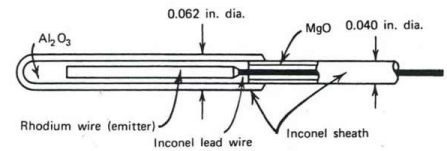
\includegraphics[width=0.5\textwidth]{img/SPD_1.png}
    \caption{Samo-napájecí detektory.}
    \label{fig:SPDKonstrukce}
\end{figure}

\subsubsection{Termoluminiscenční detektory}

Termoluminiscenční detektory jsou zařízení, která využívají schopnost některých materiálů uchovávat energii ionizujícího záření v podobě excitovaných elektronů. Když je materiál zahřátý, elektrony se uvolní z energetických pastí a při návratu na nižší energetickou hladinu vyzařují světlo.

Proces fungování termoluminiscenčních detektorů zahrnuje tyto kroky:

\begin{itemize}
    \item Ionizující záření excituje elektrony z valenčního do vodivostního pásu. Tyto elektrony jsou zachyceny v záchytných centrech.
    \item Zahřátím materiálu získají elektrony dostatečnou energii k uvolnění ze záchytných center.
    \item Při návratu do základního stavu emitují elektrony světlo, které je detekováno pomocí fotonásobiče.
\end{itemize}

Vyzařovaná energie je úměrná energii pohlceného ionizujícího záření, což umožňuje přesné měření dávky záření. 

Pro výrobu TLD se používají materiály jako lithium fluorid (LiF), calcium fluoride (CaF$_2$), magnesium beryllium oxide (MgBeO$_4$), a calcium sulfate dopovaný dysprosiem (CaSO$_4$(Dy)). Každý z těchto materiálů má různé citlivosti a energetické charakteristiky pro různé druhy záření.

Výhody termoluminiscenčních detektorů zahrnují:

\begin{itemize}
    \item Vysokou citlivost a přesnost měření.
    \item Širokou oblast lineární závislosti mezi dávkou a odezvou.
    \item Opakované použití díky možnosti vymazání zachycené energie zahřátím.
    \item Možnost použití materiálů s vlastnostmi podobnými lidské tkáni, což je výhodné pro lékařskou dozimetrie.
\end{itemize}

Nevýhody zahrnují citlivost na světlo a znečištění, což může ovlivnit přesnost měření. Termoluminiscenční detektory nejsou běžně používány v I\&C systémech jaderných reaktorů, ale nacházejí uplatnění v oblasti osobní dozimetrie.

\subsubsection{Aktivační detektory}

Aktivační detektory představují pasivní detektory ionizujícího záření, které se primárně používají k měření fluence neutronového záření. Tyto detektory mají obvykle tvar fólie nebo drátu a jsou vyrobeny buď z jednoho prvku, nebo z definované slitiny. Nejprve jsou detektory ozařovány v měřeném poli záření, během čehož dochází k indukci radionuklidů. Po ozáření se pomocí spektrometrie gama záření stanoví aktivity příslušných radionuklidů, což umožňuje výpočet celkové fluence neutronů.

Jednou z hlavních výhod aktivačních detektorů je, že jejich odezva není ovlivněna gama zářením, které je obvykle přítomné v poli neutronů. Dalšími přednostmi jsou malé rozměry a odolnost, což umožňuje jejich použití v aktivních zónách jaderných reaktorů. Pro detekci tepelných neutronů se často využívají materiály jako kobalt (Co), zlato (Au) a železo (Fe), zatímco pro rychlé neutrony se používají nikl (Ni), titan (Ti) a niob (Nb).

Specifickým příkladem použití je Aeroball Measurement System (AMS), který se používá v elektrárnách KWU. Tento systém využívá kuličky o průměru 1,7 mm vyrobené z oceli obsahující 1,5 \% vanadu. Kuličky se pohybují pneumatickým systémem (dusík) a slouží k týdenní kalibraci ostatních neutronových detektorů.

\begin{figure}[H] 
    \centering
    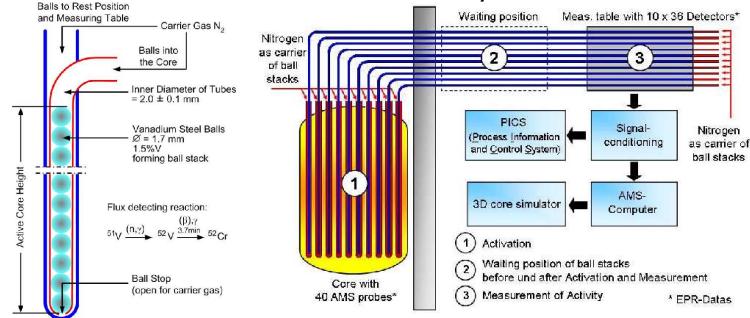
\includegraphics[width=0.5\textwidth]{img/AktivačníDetektory.png}
    \caption{Aktivační detektory v reaktoru.}
    \label{fig:AktivačníDetektory}
\end{figure}

\subsection{Charakteristiky detektorů}

\textbf{Citlivost} \textendash{} Schopnost produkovat měřitelný signál pro daný typ částic a energii. Závisí na:
\begin{itemize}
    \item účinném průřezu ionizujících interakcí,
    \item hmotnosti detektoru,
    \item šumu detektoru,
    \item tloušťce detektoru.
\end{itemize}

\textbf{Odezva} \textendash{} Vztah mezi energií částice a výstupem na detektoru (celkovým nábojem nebo amplitudou proudového pulsu).

\textbf{Funkce odezvy} \textendash{} Spektrum monoenergetického svazku je detektorem pozorováno jako komplikovaná funkce, většinou blízká Gaussově funkci s chvostem k nižším energiím.

\textbf{Mrtvá doba} \textendash{} Doba potřebná pro vytvoření a zpracování signálu v detektoru. Velmi vysoká mrtvá doba vede k navrstvení pulzů přes sebe, což následně způsobuje spektrální posun a horší rozlišení.

\textbf{Detekční účinnost} \textendash{} Poměr mezi počtem částic vyzářených zdrojem a detekovaných detektorem (absolutní účinnost). Ta se skládá z:
\begin{itemize}
    \item vnitřní účinnosti,
    \item geometrické účinnosti (akceptance).
\end{itemize}

\textbf{Energetické rozlišení} \textendash{} Nejmenší rozlišitelný rozdíl energie $\Delta E$ mezi dvěma blízkými energiemi. U monoenergetického svazku je ideálně $\delta$-funkce, reálně pík s konečnou šířkou (většinou Gaussův tvar). Rozlišení se udává ve formě pološířky (FWHM) jako relativní rozlišení $\Delta E / E$ v \%.

\textbf{Časové rozlišení} \textendash{} Nejmenší rozlišitelný rozdíl časů, definice podobná jako u energie.

\textbf{Dráhové rozlišení} \textendash{} Nejmenší rozlišitelný rozdíl v dráze, definice obdobná jako u předchozích veličin.

\subsubsection{Parametry detektorů neutronů}

\textbf{Citlivost k neutronům} \textendash{} Závisí na:
\begin{itemize}
    \item účinném průřezu konverzního materiálu a energii neutronů,
    \item objemu a hustotě detektoru (absorpce náboje).
\end{itemize}

\textbf{Energie reakce} \textendash{} Energie uvolněná záchytem neutronu ($Q$-energie), která determinuje kinetickou energii detekovatelné částice.

\textbf{Potlačení $\gamma$ záření} \textendash{} "Průhlednost" detektoru pro $\gamma$ záření v porovnání s velikostí $Q$:
\begin{itemize}
    \item větší $Q$ zajišťuje lepší odstup od šumu a $\gamma$ záření,
    \item "průhlednost" detektoru pro $\gamma$ závisí na hustotě a $Z$ detektoru.
\end{itemize}

\textbf{Možnost získání informace o energii původního neutronu} \textendash{} Kolekce celého vzniklého náboje zajišťuje spolehlivou diskriminaci a umožňuje spektroskopii. Používají se například:
\begin{itemize}
    \item konverze (n, $\alpha$),
    \item metoda odražených protonů.
\end{itemize}

\begin{table}[h!]
\centering
\caption{Parametry a jejich význam v kontextu detekce neutronů.}
\label{tab:parameters}
\resizebox{\columnwidth}{!}{
\begin{tabular}{cc}
\toprule
\textbf{Parameter}               & \textbf{Význam}                                                                                   \\ \midrule
$\Phi$ (fluence)                 & Tok neutronů (počet neutronů na jednotku plochy)                                                  \\ 
$\sigma$ (cross-section)         & Účinný průřez (pravděpodobnost interakce neutronů s látkou)                                        \\ 
$R$ (reaction rate)              & Rychlost reakcí (počet reakcí za sekundu)                                                         \\ 
$E$ (energy)                     & Energie neutronů                                                                                  \\ 
$dE/dx$ (stopping power)         & Ztráta energie na jednotku délky při průchodu částic prostředím                                   \\ 
$L$ (mean free path)             & Střední volná dráha (průměrná vzdálenost mezi interakcemi neutronů s látkou)                      \\ 
$\epsilon$ (detector efficiency) & Detekční účinnost (podíl registrovaných interakcí vůči celkovému počtu interakcí)                  \\ 
$\Delta E$ (energy resolution)   & Energetické rozlišení (schopnost detektoru rozlišit různé energie částic)                         \\ 
$T$ (time resolution)            & Časové rozlišení (schopnost detektoru rozlišit události v čase)                                   \\ 
$S/N$ (signal-to-noise ratio)    & Poměr signálu k šumu (kvalita měřeného signálu vůči šumu pozadí)                                  \\ \bottomrule
\end{tabular}
}
\end{table}

\subsection{Provozní režimy a konfigurace provozních parametrů}

\subsubsection*{Impulsní režim komory}

V impulzním režimu komory se detekují jednotlivé impulzy z neutronové komory. Signál je následně zesílen a diskriminován. Diskriminace slouží k tomu, aby byla zvýrazněna odezva na neutrony, která je nejsilnější, a naopak potlačeny impulzy s menší amplitudou, jako jsou impulzy způsobené gama, beta, alfa zářením nebo šumem. Tyto složky jsou eliminovány diskriminací. V tomto režimu je však třeba řešit problematiku mrtvé doby. Maximální četnost impulzů bývá typicky do 10$^5$ impulzů za sekundu, přičemž na zařízení VR-1 dosahuje přibližně $5 \cdot10^4$ impulzů za sekundu. Při vysokých četnostech impulzů může nastat problém stejnosměrného posunu signálu za kondenzátorem, což lze kompenzovat pomocí speciálních systémů, například systému dataPartner pro reaktor LVR-15.


\subsubsection*{Proudový režim komory}
V proudovém režimu komory se měří celkový stejnosměrný proud (DC) protékající komorou. Tento režim umožňuje potlačit mrtvou dobu, což je výhodné zejména při měření velkých hustot neutronového toku. Na druhé straně zde není možné využít standardní diskriminaci k potlačení vlivu alfa a gama záření či šumu. Proudový režim se používá pro velké rozsahy proudů, kde je vhodné využít logaritmické zesilovače nebo Campbellovu metodu, která vychází ze vztahu $n=\text{RMS}^2$. Pro potlačení vlivu gama záření se využívají kompenzované komory nebo Campbellovský režim.

\textbf{Kompenzovaná komora:}

Kompenzovaná komora se skládá ze dvou částí. První část měří jak neutrony, tak gama záření, zatímco druhá část měří pouze gama záření. Pro získání čistého signálu neutronů se odečítají proudy z obou částí podle vztahu $I_n=I_{\gamma+n}-I_{\gamma}$. Tento přístup umožňuje eliminovat vliv gama záření a získat přesné údaje o neutronovém toku

\begin{figure}[H] 
    \centering
    \includegraphics[width=0.5\textwidth]{img/KompenzovanáKomora.png}
    \caption{Kompenzovaná komora.}
    \label{fig:KompenzovanáKomora}
\end{figure}


\textbf{Campbellovský režim:}

Proudový režim, který využívá jen střídavou
složku (AC) proudu.

Campbellova metoda přináší několik významných výhod, které ji činí atraktivní pro aplikace v detekci záření. Především využití střídavých (AC) zesilovačů, které se snáze konstruují a nabízejí lepší stabilitu a menší drift ve srovnání se stejnosměrnými (DC) zesilovači.

Další výhodou je kvadratická závislost výkonu na RMS (Root Mean Square), která umožňuje pokrýt celý výkonový rozsah typicky pouze jedním měřicím kanálem.

Navíc Campbellova metoda poskytuje velmi dobrou diskriminaci gama záření, která je srovnatelná s diskriminací dosažitelnou pomocí kompenzovaných komor.

\textcolor{red}{CHYBÍ KONFIGURACE PROVOZNÍCH PARAMETRŮ!!!} 



% \section[Neutronové zdroje]{Měření základních charakteristik radionuklidových, generátorových a fotoneutronových zdrojů neutronů}

Něco je v přednášce 1 NAA, ale ně moc důkladně, lepší převzít z lepších materiálů.
% \section[Spektrometrie neutronů]{Spektrometrie neutronů pomocí Bonnerových sfér a scintilačních detektorů na bázi odražených jader}


% \section[Interakce gamma záření]{Interakce gama záření s látkou, charakteristika gama spektra, charakteristiky a kalibrace detektorů}

\subsection{Základní poznatky}

\subsubsection{Zdroje fotonů}

Hlavním zdrojem gamma fotonů je RA rozpad částic (primárně $\beta$, pro vyšší $Z$ i $\alpha$). Nově vzniklá jádra jsou nestabilní a energie se zbavují za pomoci vyzáření gamma fotonu o specifické energii a intenzitě. Tato energie je charakteristická pro daný izotop, a ačkoliv je gamma foton vyzářen nově vzniklým jádrem, v tabulkách se připisuje k původnímu nestabilnímu jádru (např. $^{90}$Sr se rozpadá na $^{90}$Y, gamma foton vyzáří $^{90}$Y, ale v tabulkách ho najdu u $^{90}$Sr). Tento proces je velmi rychlý, pokud k němu nedojde do XX sekund, tak se vzniklé izotopy označují jako \textbf{metastabilní stavy}.

Mimo to jsou s produkcí gamma fotonů spojeny další procesy související s RA rozpady:

\begin{itemize}
    \item $\beta^+$ rozpad -- vzniká pozitron, který je ihned zastaven v látce. Najde kamaráda elektron, čímž vzniká \textbf{pozitronium} (neboli krátce žijící vazba pozitronu a elektronu), anihiluje a vznikají 2 fotony o energii 511 keV jdoucí od sebe pod úhlem 180° (mohou vzniknout i 3 fotony, viz níže), tzv. \textbf{anihilační záření}. Jelikož před anihilací nezastaví pozitron uplně na nulu, je vzniklý peak rozmazaný.
    \item EC -- vzniká vakance v orbitale (nejčastěji K), která je zaplněna kaskádovými přeskoky z vyšších orbitalů, čímž vzniká charakteristické \textbf{RTG záření} (nebo Augerův elektron).
    \item IC -- neboli vnitřní konverze, nestabilní jádra se mohou energie zbavit tak, že vnitřně předají energii elektronům v obale. Ten je uvolněn, vzniká vakance, která je opět kaskádami zaplněna za vzniku charakteristického \textbf{RTG záření} (nebo Augerova elektronu).
\end{itemize}

K tomu navíc existuje:

\begin{itemize}
    \item \textbf{okamžité záření} -- vzniká v důsledku jaderných reakcí, např. (n,$\gamma$), tedy gamma fotony uvolněné hned v rámci reakce, nikoliv následný rozpad (může přesahovat až 10 MeV).
    \item \textbf{brzdné záření} -- vzniká, pokud na nabitou částici působí zrychlení (zatáčí vlivem magnetického pole, k čemuž postačí Coulombovské pole vzbuzené jádrem), což je doprovázeno ztrátou energie ve formě brzdného záření. Záření je spojité a přispívá k nárůstu kontinua v gamma spektru. Záření je vyšší pro vyšší $Z$, proto by v oblasti detektoru měly být lehké materiály.
\end{itemize}

\subsubsection{Členění fotonů}

\begin{itemize}
    \item \textbf{RTG fotony} -- vznikají v orbitalech přeskoky elektronů. Energie je dána rozdílem energií orbitalů, což je dáno hlavním a vedlejším kvantovým číslem. Nicméně elektron nemůže skákat jen tak, řídí se Paulovým vylučovacím principem, který jasně říká, v jakém pořadí se elektrony zaplňují. Nižší energie, do desítek keV. Záření je čárové a charakteristické, ale ke každému izotopu existuje spoustu peaků, jelikož záleží na přesném módu přestupu (K$_{\alpha1}$, K$_{\alpha2}$ apod.).
    \item \textbf{Gamma fotony} -- vznikají deexcitací jádra. Opět čátové charakteristické záření, ale je zde výrazně méně možností (žádné módy). Energie je vyšší, až jednotky MeV.
    \item[-] V oblasti 1 MeV se fotony překrývají, členění není tak striktní.
\end{itemize}

\subsection{Interakce gamma záření s látkou}

Fotony jsou EM záření, kterému přísluší kvantum energie dle:

$$ E_\gamma = h \nu = h \dfrac{c}{\lambda}. $$

Vlnové délky se pohybují řádově $\lambda << 10^{-10}$ m, což je výrazně méně než meziatomové vzdálenosti v mřížce. Někdy se chová jako vlna (fotoefekt), jindy jako kulička (Comptonův rozptyl).

Jelikož nejde o nabité částice (tzv. \textbf{nepřímo ionizující záření}), tak se při detekci musí spoléhat na konverzi a detekují se až sekundární částice (elektrony).

Typ interakce je podmíněný energií (např. k tvorbě páru nedojde, je-li energie pod 1022 keV). 

\textbf{Koeficient zeslabení} = charakterizuje zeslabení způsobené absorbcí v daném materiálu (osa $y$) v závislosti na energii (osa $x$). Jde o součet křivek zeslabení způsobených fotoefektem, omptonovým rozptylem a tvorbou páru.

\textbf{Absorbční koeficient} = podíl energie pohlcené absorbčním materiálem při průchodu gamma záření, jelikož ne každá interakce vede na absorbci celé energie primárního fotonu.

\subsubsection{Primární interakce}

Máme 3 základní a nejdominantnější primární interakce: fotoefekt, Comptonův rozptyl a tvorba párů. Zbytek interakcí je z pohledu detekce zanedbatelný. Tím vznikají sekundární nabité částice (elektrony), které je možné detekovat.

Celkovou pravděpodobnost interakce (mikroskopický účinný průřez $\tau$, $\sigma$ a $\kappa$) je pak možné převést do \textbf{lineárního koeficientu zeslabení}, který vyjadřuje pravděpodobnost interakce na jednotku dráhy (makroskopický účinný průřez $\mu$). 

Z toho vychází i \textbf{střední volná dráha} $\lambda$:

$$ \lambda = \dfrac{1}{\mu}, $$

a \textbf{zeslabovací zákon}:

$$ \boxed{ \dfrac{I(x)}{I_0} = e^{-\mu x}. } $$

Pokud je vzorek emitující fotony tlustý (tloušťka $L$), dochází k samostnínění (část fotonů se pohltí) a celková intenzita se musí určit integrací:

$$ \boxed{ I_\gamma(L) = \dfrac{1}{L} \int_0^L I_\gamma^0 e^{-\mu x} \: \text{d}x = \dfrac{I_\gamma^0}{\mu L} \left( 1 - e^{-\mu L} \right).} $$

V tabulkách se pak uvádí \textbf{hmotnostní koeficient zeslabení}, který je svázaný s hustotou materiálu:

$$ \mu(\text{cm}^2{\text{/g}}) = \dfrac{\mu(\text{1/cm})}{\rho(\text{g/cm}^3)}. $$

\begin{figure}[H]
    \centering
    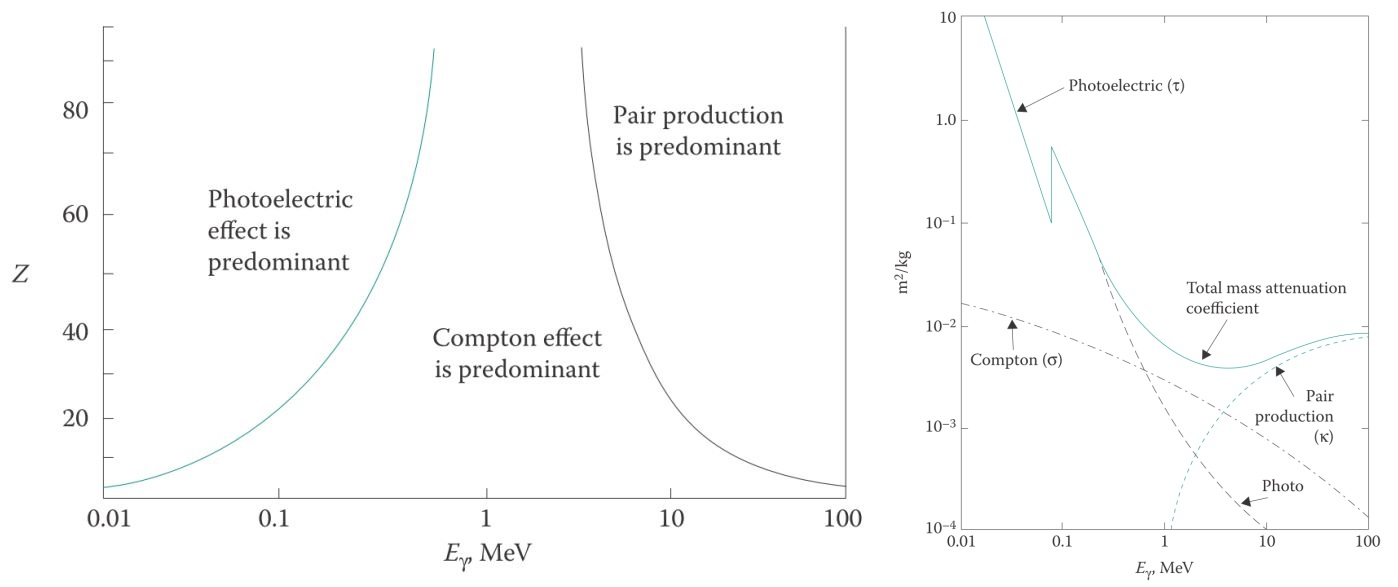
\includegraphics[width=1\textwidth]{img/interakce.JPG}
\end{figure}

\textbf{Fotoefekt:} jde o jev, kdy primární foton interaguje s elektronem v obalu, odevzdá mu veškerou svoji energii, foton zanikne a tzv. fotoelektron je uvolněn (energie fotonu $E_\gamma$ se rozdělí na vazebnou energii elektronu $E_b$ a kinetickou energii elektronu $E_e$):

$$ E_e = E_\gamma - E_b. $$

Jde o dominantní reakci při absorbci do 200 keV. Pravděpodobnost rekace (účinný průřez reakce $\tau$) klesá s energií $E_\gamma$ a roste se $Z$, jako:

$$ \tau = c \dfrac{Z^n}{E_\gamma^{3,5}}, \: \: \: n \in (4,5). $$

Energetické spektrum fotoelektronů (sekundární částice) je \textbf{čárové} a fotoefekt je zodpovědný za \textbf{peak úplného pohlcení}. Fotoelektrony mohou být uvolněny z libovolného orbitalu (nejpravděpodobněji K orbital), nicméně při nižší energii než $E_{V_K}$ už foton není schopný vyrazit elektron z K orbitalu, $\tau$ skokově klesá a dochází k vyrážení z vyšších orbitalů.

\begin{figure}[H]
    \centering
    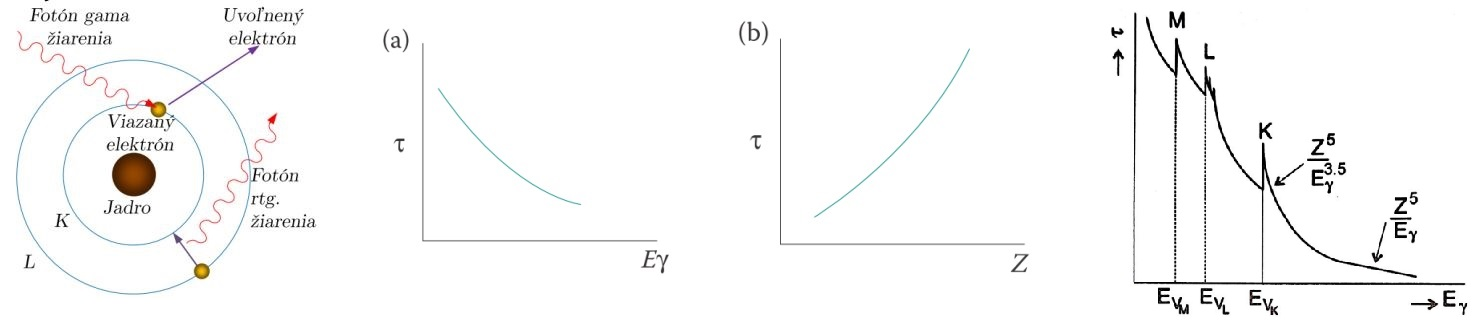
\includegraphics[width=1\textwidth]{img/fotoefekt.JPG}
\end{figure}

\textbf{Comptonův rozptyl:} jde o rozptyl fotonů na atomovém obale. Foton se odrazí od elektronu pod úhlem $\theta$ s novou energií (resp. vlnovou délkou) dle vztahu:

$$ E_\gamma' = \dfrac{E_\gamma}{1 + \dfrac{E_\gamma}{m_\text{e}c^2}(1 - \text{cos}(\theta))}. $$

Dochází k němu pro všší energie, pokud je energie nalétávajícího fotonu vyšší, než vazebná energie elektronu v obalu. Pravděpodobnost interakce (účinný průřez $\sigma$) je úměrná $Z$ a nepřímo úměrná energii $E_\gamma$:

$$ \sigma \sim \dfrac{Z}{E_\gamma}. $$

Tím vznikají odražené elektrony (sekundární částice), které jsou detekovány. Energetické spektrum odražených elektronů je \textbf{spojité}, tzv. \textbf{Comptonovo kontinuum}. To je zakončeno \textbf{Comptonovou hranou}, která je dána maximální energií elektronů (k tomu dojde, dojde-li k čelní srážce, kdy $\theta = 180°$).

Úhlová sitribuce rozptýlených fotonů je dána Klein-Nishinovým vztahem pro diferenciální účinný průřez, s rostoucí energií gamma fotonů roste pravděpodobnost dopředných úhlů.

\begin{figure}[H]
    \centering
    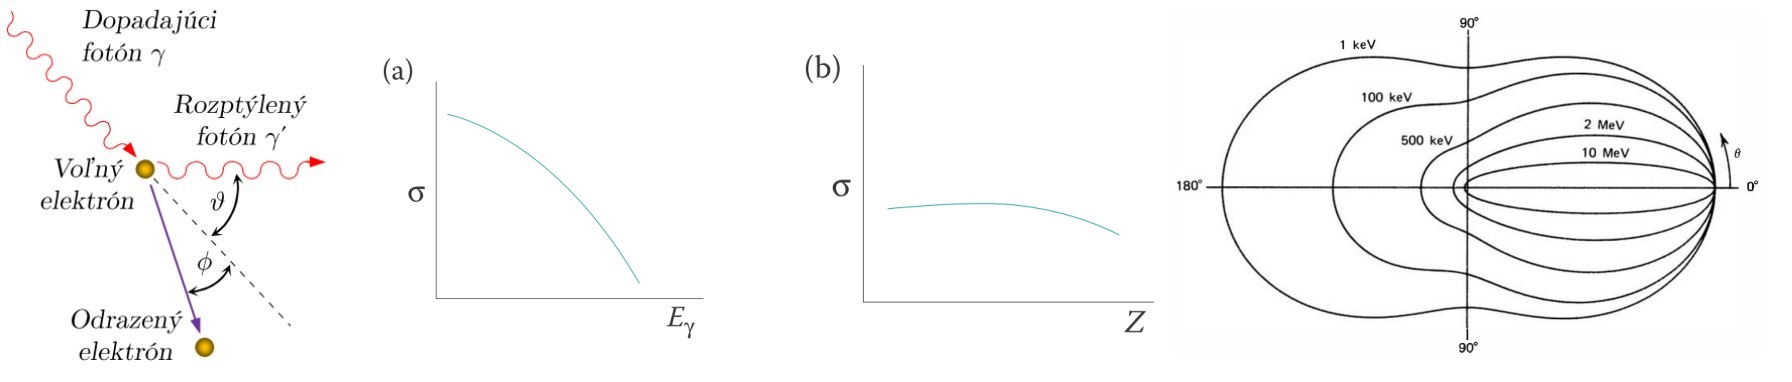
\includegraphics[width=1\textwidth]{img/Compton.JPG}
\end{figure}

\textbf{Tvorba elektron-pozitron páru:} jde o důsledek interakce gamma fotonu s jádrem. Dojde k zaniknutí gamma fotonu a vznikne pár elektron-pozitron o energiích:

$$ E = \dfrac{1}{2} (E_\gamma - 1022 \text{ keV}). $$

Elektron i pozitron se ihned zastaví a v případě pozitronu dojde ke vzniku pozitronia, anihilaci a vzniku 2-3 fotonů.

Pravděpodobnost interakce (účinný průřez $\kappa$) roste s energií $E_\gamma$ a je přímo úměrná $Z^2$. Zároveň jde o prahovou reakci a je dominantní pro vysoké energie:

$$ \kappa \sim Z^2 \: \text{ln} \left( \dfrac{E_\gamma}{m_\text{e} c^2} \right). $$

\begin{figure}[H]
    \centering
    \includegraphics[width=0.7\textwidth]{img/pár.JPG}
\end{figure}

\textbf{Fotojaderné reakce:} při interakci a pohlcení gamma fotonů může být z jádra emitován nukleon.

Jde o prahové reakce a je jich spousta: ($\gamma$,n), ($\gamma$,2n), ($\gamma$,p), ($\gamma$,np), ($\gamma$,$\alpha$) apod. Jde o prahové reakce (alespoň 5 MeV), v porovnání s předchozími 3mi reakcemi jsou zanedbatelné. Problematické v radiační ochraně (emitují se těžké nabité částice).

V JI se využívají hlavně k emitování neutronů, jako fotojaderné neutronové zdroje (např. $^{206}$Pb, $^{9}$Be, $^2$H, $^{7}$Li, $^{14}$N apod.)

\textbf{Rayligho rozptyl:} jde o koherentní rozptyl fotonu s celým obalem (tedy se všemi elektrony), přičemž nedochází k ionizaci, ani excitaci (nepřenáší se enegie, vlnová délka fotonů se zachovává). Pouze se mění směr hybnosti fotonů.

Opět nepříliš dominantní interakce, lze zanedbat. Roste pro nízké energie fotonů a vysoká $Z$. Vsuvka, vysvětluje, proč je obloha modrá (ale nevim proč :D).

\subsubsection{Druhotné efekty}

V případě detekce může docházet k zaznamenávání nechtěných druhotných efektů.

\textbf{Vícenásobná interakce:} Comptonovsky rozptýlené fotony v citlivé oblasti detektoru mohou znovu interagovat (fotoefektem, Comptonovsky), což může přispět do peaku úplné absorbce, nebo vytvořit novou Comptonovu hranu.

\textbf{Peak zpětného rozptylu:} fotony proletí detektorem bez interakce, Comptonovsky interagují až v okolním materiálu, rozptýlí se zpět s nižší energií do citlivé oblasti detektoru a jsou zaregistrovány. Tím vzniká peak zpětného rozptylu s nižší energií.

\textbf{Anihilace elektron-pozitron:} pokud mimo detektor dojde ke tvorbě páru, vzniklý elektron a pozitron za vzniku pozitronia anihilují a jeden z fotonů se dostane zpět do detektoru. Absorbcí fotoefektem vzniká anihilační peak 511 keV.

\textbf{Pozitronium} je vázaný systém, analogický atomu vodíku, kdy elektron a pozitron obíhají kolem společného těžiště s dobou života okolo 10$^{-10}$. Existují 2 typy v závislosti na spinu:

\begin{itemize}
    \item Para-pozitronium -- spiny opačně, vznikají 2 fotony o energii 511 keV (dominantní),
    \item Orto-pozitronium -- spiny shodně, vznikají 3 fotony (málo časté).
\end{itemize}

\textbf{RTG záření:} je způsobené fotoefektem, kdy je vzniklá vakance zaplněna jiným elektronem a vyzářením RTG záření.

\textbf{Augerovy elektrony:} konkurenční proces k RTG záření, pouze je přebytečná energie předána sousednímu elektronu, který je uvolněn a vyletí ven.

\textbf{Brzdné záření:} vzniká, pokud elektrony a pozitrony proletí kolem jádra, které vyvolává Coulombovo EM pole.

\textbf{Sumační efekty:} ovlivněno geometrií detektoru, můžou být zaznamenány 2 gamma kvanta ve stejný okamžik (např. 511 keV + gamma deexcitace)

\textbf{Pozadí:} detektor detekuje záření z přirozeného prostředí, jde hlavně o izotopy $^{40}$K, $^{137}$Cs a produkty rozpadových řad (urany, radony apod.). Lze zamezit dobrým stíněním.

\subsection{Charakteristika gamma spektra}

\subsubsection{Tvar gamma spektra}

Spektrum, které zaznamenám, je dáno vlastnostmi detektoru.

\textbf{Limitní případ malého detektoru:} nastává, pokud střední volná dráha sekundárních fotonů (řádově jednotky cm) je výrazně větší, než citlivá plocha detektoru (do 1-2 cm). Detektor tak zaznamená pouze primární interakce, nedochází k vícenásobné interakci. Sekundární fotony vyletí ven.

Za předpokladu, že detektor zaznamená veškerou energii sekunádrních elektronů, tak se spektrum projeví Comptonovým kontinuem zakončeným Comptonovou hranou (Comptonův rozptyl) a fotopeakem úplné absorbce (fotoefekt, vznikne \textbf{FEP = Full Energy Peak}). 

Pro energie větší než 1022 keV se navíc projeví efekt tvorby párů (vznikne \textbf{DEP = Double Escape Peak}), anihilační fotony (jde o sekundární fotony) uniknou.

$$ E_\text{DEP} = E_\text{FEP} - 2 \cdot 511 \text{ keV}. $$

\begin{figure}[H]
    \centering
    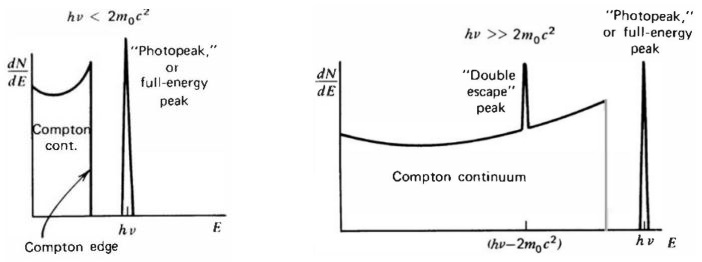
\includegraphics[width=0.7\textwidth]{img/maly_detektor.JPG}
    \caption{Tvar gamma spektra pro malý detektor ($E_\gamma < 1022$ keV vlevo, $E_\gamma > 1022$ keV vpravo).}
\end{figure}

\textbf{Limitní případ velkého detektoru:} pokud je střední volná dráha sekundárních fotonů výrazně menší, než rozměry detektoru. Ten pak zaznamená veškeré interakce, nic neunikne. Nakonec pak vždy dojde k fotoabsorbci, veškerá energie primárního záření je doponována v detektoru, tudíž zaznamenaný náboj sekundárních elektronů odpovídá energii primárního záření. Výsledná odezva je stejná, jako by primární gamma záření interagovalo pouze fotoefektem.

Spektrum se projevuje pouze peakem úplné abosrbce FEP, v tomto případě \textbf{peak úplného pohlcení}.

\begin{figure}[H]
    \centering
    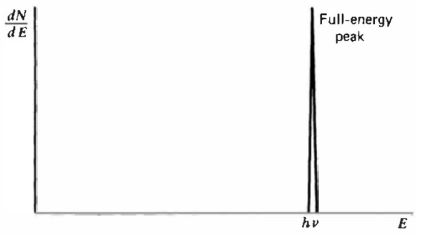
\includegraphics[width=0.4\textwidth]{img/velky_detektor.JPG}
    \caption{Tvar gamma spektra pro velký detektor.}
\end{figure}

\textbf{Středně velký detektor:} Ve skutečnosti vždy něco vylétne (kor, pokud dojde k reakci na kraji detektoru), tudíž reálný detektro zaznamená něco mezi. Nízkoenergetické záření se zaznamená lépe, jelikož nedochází tak často k sekundárním interakcím. Pak dochází k vícenásobným Comptonovým rozptylům, které vyplňují mezeru mezi Comptonovou hranou a fotopíkem.

Pro energie větší než 1022 keV se opět projevuje DEP, ale navíc i \textbf{SEP = Single Escape Peak} (pokud jeden foton unikne, a druhý ne).

$$ E_\text{SEP} = E_\text{FEP} - 511 \text{ keV}. $$

\begin{figure}[H]
    \centering
    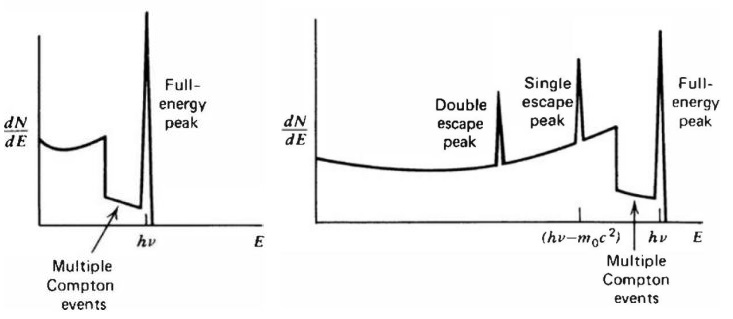
\includegraphics[width=0.7\textwidth]{img/stredni_detektor.JPG}
    \caption{Tvar gamma spektra pro středně velký detektor ($E_\gamma < 1022$ keV vlevo, $E_\gamma > 1022$ keV vpravo).}
\end{figure}

V každém případě nedojde k deponování veškeré energie a některé sekundární fotony uniknou, tento efekt nárůstá s energií těchto fotonů. To způsobuje zkreslení odezvové funkce a některé události jsou posunuty do nižších energií.

$\rightarrow$ \textbf{Ve zkratce.} Pokud mi nic neunikne, objeví se pouze FEP. Reálně ale něco unikne, což se projeví ve formě SEP a DEP (uniklé anihilační fotony). Pokud je detektor hodně malý, tak unikne vše sekundární a projeví se pouze DEP.

Ideálně chceme znát pouze FEP, přičemž Comptonovo kontinuum nám zkresluje měření. Pro jeho potlačení je možné využít koincidenční nebo antikoincidenční zapojení vícera detektorů a detekovat pouze určité interakce (v tomto případě FEP):

\begin{itemize}
    \item Comptonův spektrometr -- gamma-gamma spektrometr, mám 2 detektory pod úhlem $\theta$ a matematickým postprocessingem Comptonovo kontinuum eliminuju.
\end{itemize}

\subsubsection{Další efekty}

\textbf{RTG únikové peaky:} ty jsou způsobeny tím, že uniknou RTG fotony, které vzniknou kaskádou po fotoefektu (tzv. \textbf{XEP = X-ray Escape Peak}). V případě nekonečně velkého detektoru neuniknou a opět se veškerá energie deponuje v FEP.

$$ E_\text{XEP} = E_\text{FEP} - E_\text{X}. $$

\textbf{Anihilační peaky:} projeví se hlavně, je-li zářič $\beta^+$ radioaktivní. Pozitron anihiluje v materiálu a vzniknou gamma fotony o 511 keV. Pokud neuniknou, projeví se ve formě FEP na energii právě 511 keV. Pokud zaznamenáváme celou prostorovou geometrii, tak se projeví ve formě FEP na energii 1022 keV (zaznamenám oba dva najednou).

\textbf{Brzdné záření:} pokud máme gamma zářič $\beta$ radioaktivní, mohou unikat $\beta$ částice přímo ze zdroje a za vzniku brzdného záření zkreslovat spektrum. K tomu se používají filtry ($\beta$ absorbátory) z lehkých materiálů, které je pohltí (např. Be).

\textbf{Okolní materiály:} tvar gamma spektra a jeho zkreslení mohou ovlivňovat i okolní materiály, s kterými záření může interagovat (stínění, pouzdro, materiál zářiče, zpětně rozptýlené gamma, sumační peaky apod.)

\begin{figure}[H]
    \centering
    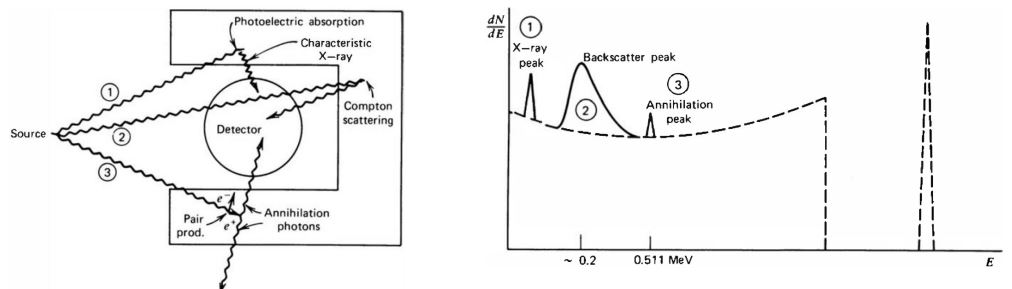
\includegraphics[width=0.9\textwidth]{img/vliv_materialu.JPG}
    \caption{Vliv okolních materiálů na tvar gamma spektra.}
\end{figure}

\subsubsection{Měření}

Při měření se projevuje statistika. My jsme v rámci detekce schopni zaznamenat histogramový záznam v jednotlivých energetických kanálech. Pod 100 zaznamenaných událostí je třeba uvažovat Poissonovo rozdělení, nad 100 událostí Gaussovo rozdělení (čas vs. aktivita). 

Ve výsledku poté zaznamenáme celkovou plochu pod peakem $S$ s potlačením Comptonova kontinua a pozadí pod peakem a s nejistotou, kterou určím z matematického popisu Gaussiánu. Dále se určí statistická významnost dle:

\begin{itemize}
    \item kritický limit $L_C$ -- plocha $S$ musí být větší než minimální hodnota,
    \item horní limit $L_U$ -- hodnota, kterou by plocha $S$ neměla překročit,
    \item detekční limit $L_D$ -- hodnota, nad kterou je plocha $S$ detekovatelná,
    \item limit stanovitelnosti $L_Q$ -- hodnota, nad kterou určím plochu $S$ s předem danou nejistotou.
\end{itemize}

$$ L_C < L_D < L_Q < S < L_U $$

\textbf{MDA} = Minimální detekovatelná aktivita, jde o nejmenší aktivitu, které může být s jistoutou měřené.

\subsection{Detektory gamma záření}

\subsubsection{Základní typy detektorů}

\textbf{Scintilační detektory:}

\begin{itemize}
    \item[1)] Primární gamma záření putuje do scintilačního krystalu, absorbuje se a část záření se transformuje na záblesk viditelného světla (\textbf{luminiscence}, atomy jsou excitovány a deexcitují viditelnými fotony), energie je úměrná světelnému signálu.
    \item[2)] Fotony putují fotonásobičem (elektronka), který mění světlo na elektrický signál. Ve formě fotokatody na vstupu, ze které jsou fotoefektem emitovány elektrony (to je ten signál).
    \item[3)] Na výstupu je anoda a vzniklé napětí urychluje elektrony za vzniku elektrického proudu. elektrony postupně dopadají na dynody, na kterých jsou vyráženy nové elektrony (2-6) a signál je zesilován. Je možné zesílit intenzitu elektronů až o 5 řádů.
    \item[4)] Takto zesílený proud je již detekovatelný, je vyveden na pracovní odpor, na kterém se mění napětí (to je ten signál, který měřím). 
\end{itemize}

\begin{figure}[H]
    \centering
    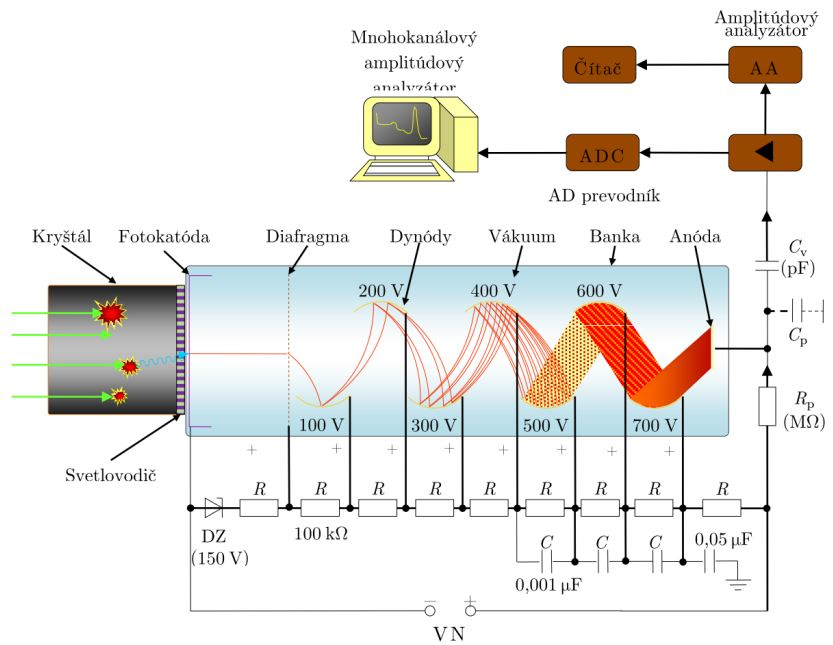
\includegraphics[width=0.65\textwidth]{img/scintilak.JPG}
    \caption{Princip scintilačního detektoru.}
\end{figure}

Scintilační krystal může být:

\begin{itemize}
    \item \textbf{Anorganický} -- primárně pro spektrometrii (gamma). 
    \item[-] Krystal je tvořen nejčastěji alkalickými kovy s malou příměsí nečistoty (tzv. aktivátor, to co je v závorce a ten je zodpovědný za luminiscenci): NaI(Tl), CsI(Tl), CaI(Na), LiI(Eu), CaF$_2$(Eu). 
    \item[-] Pro nízkoenergetické je lepší krystal s malým $Z$, pro vysokoenergetické s velkým $Z$ (ale tam je potom menší energetická rozlišitelnost).  
    \item \textbf{Organický} -- primárně pro neutrony a nabité částice.
    \item[-] Krystal je tvořen organickými molekulami na bázi benzenu a luminiscence je způsobena molekulárními deexcitacemi.
    \item[] Mohou být krystaly (antracen), kapaliny (rozpouštědlo + org. aktivátor, např. toluen + p-terphenyl), plasty (org. aktivátor v polymeru)
\end{itemize}

\textbf{Polovodičové detektory:}

\begin{itemize}
    \item[1)] Ve formě diody z čistého polovodiče v závěrném směru. Gamma záření způsobuje vyrážení elektronů, které se dostávají do vodivého pásma.
    \item[2)] Vznikají tak páry elektron-díra, které jsou nosičemi náboje, čímž vzniká elektrický signál.
    \item[3)] Ten putuje do předzesilovače, zesilovače, tvaruje se a zaznamenává v MCA.
\end{itemize}

Mají mnohem lepší energetickou rozlišitelnost, ale jsou dražší a musejí se chladit (jinak elektrony vyskakují samy a vzniká tak šum). Momentálně nejlepším detektorem je superčistý krystal germania (HPGe).

\textbf{Rozdíly:} polovodičové detektory mají lepší energetickou rozlišitelnost, ale menší detekční účinnost. Také jsou levnější.

\subsubsection{Základní charakteristiky}

\textbf{Odeva detektoru:} poměr mezi energií záření a pozorovaným výstupem (binem) na detektoru (záření o energii $E$ vytvoří $N$ nosičů náboje, které způsobí napěťový rozdíl na elektrodách detektoru, což je to, co detektor zaznamená).

\textbf{Odezvová funkce:} vyjadřuje pravděpodobnost, že monoenergetické fotony budou zaznamenané v daném energetickém binu.

\textbf{Časová odezva detektoru:} čas potřebný k vytvoření signálu. Signál je ve tvaru ostré náběžné a pozvolné seběžné hrany.

\textbf{Časové rozlišení:} nejmenší časová rozlišitelnost mezi dvěmi signály.

\textbf{Citlivost detektoru:} schopnost detektoru produkovat měřitelný signál pro konkrétní typ částice s danou energií. závisí na účinných průřezech, rozměrech hmotnosti, materiálech, šumu (ten může růst s rostoucím rozměrem detektoru).

\textbf{Mrtvá doba:} čas potřebný na zpracování signálu.

\textbf{Energetické rozlišení} nejmenší energetická rozlišitelnost mezi dvěmi signály. Detektor s dobrým rozlišením má užší a vyšší peak, než detektor s horším rozlišením (ale plochy pod peakem jsou stejné).

\textbf{FWHM} = Full Width at Half Maximum, stanovuje šířku pulzu (peaku) v polovině jeho maxima. Dáno energetickým rozlišením. Z toho je možné stanovit relativní energetické rozlišení jako:

$$ R = \dfrac{\text{FWHM}}{E}. $$

Polovodičové detektory mají $R \approx 1$ \%, scintiláky $R \approx 3-10$ \%.

\textbf{Detekční účinnost:} poměr mezi počtem registrovaných částic a emitovaných částic.

\subsubsection{Kalibrace detektorů}

\textbf{Kalibrace energetického rozlišení:} za pomoci FWHM. Peak si proložím Gaussiánem, určím FWHM a relativní rozlišení. Problém nastává, pokud se peaky překrývají (tzv. \textbf{multiplety}).

\textbf{Energetická kalibrace:} MCA mi dá histogram, který musím zkalibrovat (až 16 tisíc kanálů). Jednotlivým binům za pomoci kalibračních zářičů přiřadím konkrétní energii, přičemž předpokládám lineární závislost (pokud mám více zářičů, je možné uvažovat kvadratickou závislost).

\textbf{Kalibrace na mrtvou dobu:} Pokud máme příliš vysokou mrtvou dobu, dochází ke ztrátám počítání signálů a ke ztrátě informací (větší aktivita může vést k přehlcení detektoru a k nárůstu mrtvé doby). Rozlišujeme:

\begin{itemize}
    \item Nekumulativní mrtvá doba -- události, které nastaly v průběhu mrtvé doby, nejsou zaznamenány, ale nevedou na prodloužení celkové mrtvé doby.
    \item Kumulativní mrtvá doba -- události, které nastaly v průběhu mrtvé doby, nejsou zaznamenány, ale vedou na prodloužení celkové mrtvé doby
\end{itemize}

\begin{figure}[H]
    \centering
    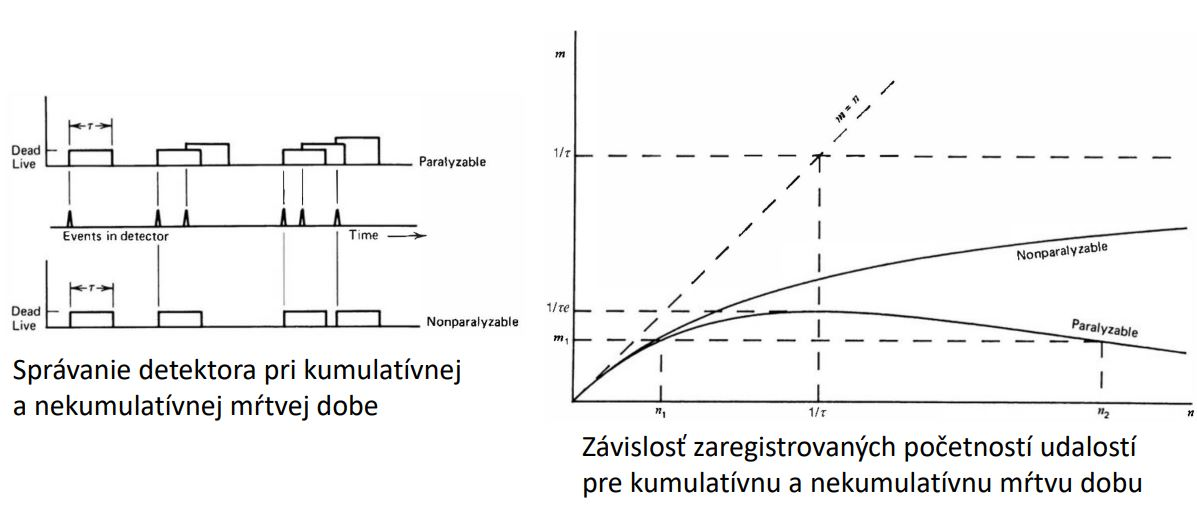
\includegraphics[width=0.8\textwidth]{img/mrtva_doba.JPG}
    \caption{Analýza mrtvé doby.}
\end{figure}

\textbf{Kalibrace detekční účinnosti:} ta není konstantní, je závislá na energii a typu záření. Je zapotřeba stanovit funkci detekční účinnosti za pomoci etalonů o známé aktivitě.

\begin{figure}[H]
    \centering
    \includegraphics[width=0.8\textwidth]{img/detekcni_krivka.JPG}
\end{figure}

\textbf{Aplikace opravných faktorů:} na závěr je vhodné uvažovat opravné faktory:

\begin{itemize}
    \item oprava na RA rozpad (zářič se v průběhu měření rozpadá),
    \item oprava na nebodovost zdroje,
    \item oprava na samostínění (pro vzorky konečné tloušťky),
    \item oprava na náhodné koincidence (potlačení sumačních efektů).
\end{itemize}

Pak je možné určit finální aktivitu vzorku z analýzi FEP (v pořadí korekce na samostínění, korekce na rozpad a celková aktivita peaku):

$$ \boxed{ A = \dfrac{\mu L}{1 - e^{-\mu L}} \dfrac{\lambda t_\text{real}}{1 - e^{- \lambda t_\text{real}}} \dfrac{S}{I_\gamma \: \varepsilon_\text{FEP}^\text{abs} \: {t_\text{live}}}.} $$



\end{document}
